%  A simple AAU report template.
%  2015-05-08 v. 1.2.0
%  Copyright 2010-2015 by Jesper Kjær Nielsen <jkn@es.aau.dk>
%
%  This is free software: you can redistribute it and/or modify
%  it under the terms of the GNU General Public License as published by
%  the Free Software Foundation, either version 3 of the License, or
%  (at your option) any later version.
%
%  This is distributed in the hope that it will be useful,
%  but WITHOUT ANY WARRANTY; without even the implied warranty of
%  MERCHANTABILITY or FITNESS FOR A PARTICULAR PURPOSE.  See the
%  GNU General Public License for more details.
%
%  You can find the GNU General Public License at <http://www.gnu.org/licenses/>.
%
% Document class, language and encoding setup
\documentclass[twoside,12pt,english]{article}
\usepackage[top=25mm,bottom=25mm,left=30mm,right=40mm]{geometry}
\usepackage[english]{babel}
\usepackage[utf8]{inputenc}
\usepackage[T1]{fontenc}
% Fixing the font issue
\usepackage{ae,aecompl}

%All empty pages have no page style
\usepackage{emptypage}

% Color package
\PassOptionsToPackage{dvipsnames}{xcolor}
	\RequirePackage{xcolor} % [dvipsnames] 
	
% Allows page-links in pdf file
\usepackage{hyperref}
\hypersetup{
% Uncomment the line below to remove all links (to references, figures, tables, etc)
%draft, 
%colorlinks=true, linktocpage=true, pdfstartpage=3, pdfstartview=FitV,
% Uncomment the line below if you want to have black links (e.g. for printing black and white)
colorlinks=true, linktocpage=true, pdfborder={0 0 0}, 
pdfstartpage=3, pdfstartview=FitV, hypertexnames=true, pdfhighlight=/O, 
breaklinks=true, pdfpagemode=UseNone, pageanchor=true, pdfpagemode=UseOutlines, plainpages=false,
bookmarksnumbered, bookmarksopen=true, bookmarksopenlevel=1,
urlcolor=Black, linkcolor=Black, citecolor=Black,
%------------------------------------------------
% PDF file meta-information
%pdftitle={\myTitle},
%pdfauthor={\textcopyright\ \myName, \myUni, \myFaculty},
%pdfsubject={},
%pdfkeywords={},
%pdfcreator={pdfLaTeX},
%pdfproducer={LaTeX with hyperref and classicthesis}
%------------------------------------------------
}

% Todo notes package and commands
\usepackage[colorinlistoftodos]{todonotes}

% Allows commands to emit a space "at the end"
\usepackage{xspace}

% Listings setup
\usepackage{listings}

% Algorithm2e
\usepackage[lined,boxed,commentsnumbered,linesnumbered]{algorithm2e}

% Graphics setup
\usepackage{graphicx}
\graphicspath{{./grafik/}}

%Til subfigure brug
\usepackage{caption}
\usepackage{subcaption}

\usepackage{tikz}
\usetikzlibrary{arrows,calc,positioning,shapes.geometric}

\usepackage{amsmath}
\usepackage{amssymb}

% Clever references
\usepackage{cleveref}

% Named references
\usepackage{nameref}

% Bibliography
\usepackage[square,numbers]{natbib}
\bibliographystyle{unsrtnat}

% Force position [H]
\usepackage{float}

\usepackage{verbatim}

% Additional commands
\newcommand{\namedtodo}[5]
{
  \ifthenelse{\equal{#1}{}}
  {
    \todo[backgroundcolor=#4,caption=
    {\textbf{#3: } #2}
    ,inline]
    {\color{#5}\textbf{#3: }#2}
  }
  {
    \todo[backgroundcolor=#4,caption=
    {\textbf{#3: } #1}
    ,inline]
    {\color{#5}\textbf{#3: }#2}
  }
}
\newcommand{\mikkel}[2][]{\namedtodo{#1}{#2}{Mikkel}{blue!80}{white}}
\newcommand{\stefan}[2][]{\namedtodo{#1}{#2}{Stefan M}{orange}{black}}
\newcommand{\mikael}[2][]{\namedtodo{#1}{#2}{Mikael}{green}{black}}
\newcommand{\bruno}[2][]{\namedtodo{#1}{#2}{Bruno}{black!10!red!90}{white}}
\newcommand{\alexander}[2][]{\namedtodo{#1}{#2}{Alexander}{black!10!yellow!90}{black}}
\newcommand{\giovanni}[2][]{\namedtodo{#1}{#2}{Giovanni}{purple!90!orange}{white}}


  \makeatletter \renewcommand \listoftodos{\section*{List of Todos} \@starttoc{tdo}}
  \renewcommand\l@todo[2]
    {\par\noindent \textit{#2}, \parbox{10cm}{#1}\par} \makeatother
% Her er en liste over navnene på de forskellige styles
% C#: csharp
% F#: fsharp

% 
% Listings kan refereres vha. \cref{}
\crefname{lstlisting}{kodeeksempel}{kodeeksempel}
\Crefname{lstlisting}{Kodeeksempel}{Kodeeksempel}
% 

%Algoritmer i cref
\crefname{algocf}{algorithm}{algorithm}
\Crefname{algocf}{Algorithm}{Algorithms}
%Algoritmelinjer i cref
\crefalias{AlgoLine}{line}%

\makeatletter
\let\cref@old@stepcounter\stepcounter
\def\stepcounter#1{%
  \cref@old@stepcounter{#1}%
  \cref@constructprefix{#1}{\cref@result}%
  \@ifundefined{cref@#1@alias}%
    {\def\@tempa{#1}}%
    {\def\@tempa{\csname cref@#1@alias\endcsname}}%
  \protected@edef\cref@currentlabel{%
    [\@tempa][\arabic{#1}][\cref@result]%
    \csname p@#1\endcsname\csname the#1\endcsname}}
\makeatother
%

% Angivelse af navn på listings
\renewcommand\lstlistingname{Kodeeksempel}
\renewcommand\lstlistlistingname{Kodeeksempel}

\lstdefinestyle{standard}
{
	frame=shadowbox,
	framesep=5pt,
	rulecolor=\color{blue!40!black},
	rulesepcolor=\color{white!93!black},
	numbers=left,
	basicstyle=\ttfamily,
	numberstyle=\tiny,
	numberfirstline=true,
	%numberblanklines=false,
	stepnumber=1,
	numbersep=9pt,	
	captionpos=b,
	escapeinside={(*}{*)},
	breaklines=true,
	tabsize=4,
	language=c,
	showstringspaces=false
}

\lstset{style=standard}

\lstdefinestyle{c}
{
	style=standard
}

\lstdefinestyle{csmall}
{
	style=c
}

\lstdefinestyle{csharp}
{
	style=standard,
	language=[Sharp]C
}
\lstdefinestyle{csharpsmall}
{
	style=csharp
}
\lstdefinestyle{fsharp}
{
	language=[Sharp]F,
	frame=lr,
	rulecolor=\color{blue!80!black}
}
\lstdefinestyle{fsharpsmall}
{
	style=fsharp,
	basicstyle=\ttfamily\footnotesize
}


% Definitions

% Superscript and subscript
\newcommand{\superscript}[1]{\ensuremath{^{\textrm{#1}}}}
\newcommand{\subscript}[1]{\ensuremath{_{\textrm{#1}}}}

% Degrees
\newcommand{\degree}{\ensuremath{^\circ}}
\newcommand{\dg}{\degree}

\newcommand{\quoter}[1]%
{
  \par
  \vspace{1.5em}
  \addtolength{\leftskip}{1.5cm}
  \addtolength{\rightskip}{1.5cm}
  \textit{#1}
  \addtolength{\leftskip}{-1.5cm}
  \addtolength{\rightskip}{-1.5cm}
  \vspace{1.5em}
  \par
}


\newcommand{\sensor}[3]
{
	\section{#1}
	#2
	
	#3
}

\newcommand{\analyse}[2]
{
\subsection{#1}
#2
}




%Prevents weird stretching of short pages
\raggedbottom


\usepackage{multicol}

%bruges til description
\usepackage{enumitem}% package inclusion and set up of the document
% see, e.g., http://en.wikibooks.org/wiki/LaTeX/Formatting#Hyphenation
% for more information on word hyphenation
\hyphenation{ex-am-ple hy-phen-a-tion short}
\hyphenation{long la-tex}
% 
%  A simple AAU report template.
%  2015-05-08 v. 1.2.0
%  Copyright 2010-2015 by Jesper Kjær Nielsen <jkn@es.aau.dk>
%
%  This is free software: you can redistribute it and/or modify
%  it under the terms of the GNU General Public License as published by
%  the Free Software Foundation, either version 3 of the License, or
%  (at your option) any later version.
%
%  This is distributed in the hope that it will be useful,
%  but WITHOUT ANY WARRANTY; without even the implied warranty of
%  MERCHANTABILITY or FITNESS FOR A PARTICULAR PURPOSE.  See the
%  GNU General Public License for more details.
%
%  You can find the GNU General Public License at <http://www.gnu.org/licenses/>.
%
%
%
% see, e.g., http://en.wikibooks.org/wiki/LaTeX/Customizing_LaTeX#New_commands
% for more information on how to create macros

%%%%%%%%%%%%%%%%%%%%%%%%%%%%%%%%%%%%%%%%%%%%%%%%
% Macros for the titlepage
%%%%%%%%%%%%%%%%%%%%%%%%%%%%%%%%%%%%%%%%%%%%%%%%
%Creates the aau titlepage
\newcommand{\aautitlepage}[3]{%
  {
    %set up various length
    \ifx\titlepageleftcolumnwidth\undefined
      \newlength{\titlepageleftcolumnwidth}
      \newlength{\titlepagerightcolumnwidth}
    \fi
    \setlength{\titlepageleftcolumnwidth}{0.5\textwidth-\tabcolsep}
    \setlength{\titlepagerightcolumnwidth}{\textwidth-2\tabcolsep-\titlepageleftcolumnwidth}
    %create title page
    \thispagestyle{empty}
    \noindent%
    \begin{tabular}{@{}ll@{}}
      \parbox{\titlepageleftcolumnwidth}{
        \iflanguage{danish}{%
          
\includegraphics[width=.8\titlepageleftcolumnwidth]{aau_logo_da}
        }{%
          
\includegraphics[width=.8\titlepageleftcolumnwidth]{aau_logo_en}
        }
      } &
      \parbox{\titlepagerightcolumnwidth}{\raggedleft\sf\small
        #2
      }\bigskip\\
       #1 &
      \parbox[t]{\titlepagerightcolumnwidth}{%
      \textbf{Abstract:}\bigskip\par
        \fbox{\parbox{\titlepagerightcolumnwidth-2\fboxsep-2\fboxrule}{%
          #3
        }}
      }\\
    \end{tabular}
    \vfill
    \iflanguage{danish}{%
      \noindent{\footnotesize\emph{Rapportens indhold er frit tilgængeligt, men offentliggørelse (med kildeangivelse) må kun ske efter aftale med forfatterne.}}
    }{%
      \noindent{\footnotesize\emph{The content of this report is freely available, but publication (with reference) may only be pursued due to agreement with the author.}}
    }
    \clearpage
  }
}

%Create english project info
\newcommand{\englishprojectinfo}[8]{%
  \parbox[t]{\titlepageleftcolumnwidth}{
    \textbf{Title:}\\ #1\bigskip\par
    \textbf{Theme:}\\ #2\bigskip\par
    \textbf{Project Period:}\\ #3\bigskip\par
    \textbf{Project Group:}\\ #4\bigskip\par
    \textbf{Participant(s):}\\ #5\bigskip\par
    \textbf{Supervisor(s):}\\ #6\bigskip\par
    \textbf{Copies:} #7\bigskip\par
    \textbf{Page Numbers:} \pageref{LastPage}\bigskip\par
    \textbf{Date of Completion:}\\ #8
  }
}

%Create danish project info
\newcommand{\danishprojectinfo}[8]{%
  \parbox[t]{\titlepageleftcolumnwidth}{
    \textbf{Titel:}\\ #1\medskip \par
    \textbf{Tema:}\\ #2\medskip \par
    \textbf{Projektperiode:}\\ #3\medskip \par
    \textbf{Projektgruppe:}\\ #4\medskip \par
    \textbf{Deltager(e):}\\ #5\medskip \par
    \textbf{Vejleder(e):}\\ #6\medskip skip\par
    \textbf{Oplagstal:} #7\medskip \par
    \textbf{Sidetal:} \pageref{LastPage}\medskip \par
    \textbf{Afleveringsdato:}\\ #8
  }
}

%%%%%%%%%%%%%%%%%%%%%%%%%%%%%%%%%%%%%%%%%%%%%%%%
% An example environment
%%%%%%%%%%%%%%%%%%%%%%%%%%%%%%%%%%%%%%%%%%%%%%%%
\theoremheaderfont{\normalfont\bfseries}
\theorembodyfont{\normalfont}
\theoremstyle{break}
\def\theoremframecommand{{\color{gray!50}\vrule width 5pt \hspace{5pt}}}
\newshadedtheorem{exa}{Example}[chapter]
\newenvironment{example}[1]{%
		\begin{exa}[#1]
}{%
		\end{exa}
}
% my new macros


\begin{document}
%frontmatter
\pagestyle{empty} %disable headers and footers
\pagenumbering{roman} %use roman page numbering in the frontmatter
\hspace*{-1cm}\parbox[b][\textheight][t]{\textwidth}
{

\begin{center}
	
\includegraphics[height=5.2cm]{aau_logo_da}\\
	\vspace{0.25cm}
	%Student Report
\end{center} 

\vspace{1cm}
\begin{center}

\textbf{\Huge {PsyLog - En modulær mobil platform}} \\ \vspace{0.5cm}
\textbf{\Large P8 Projekt af SW807F15 og SW808F15}\\ \vspace{0.5cm}
\textbf{\large 2. februar 2015 til 27. maj 2015}\\
\end{center}



\vspace{0.25cm}
\begin{center}
\item {\textbf{Deltagere:}} \\
\textbf{SW807:}\\
Bruno Thalmann\\
Mikael Elkiær Christensen\\
Mikkel Larsen\\
Stefan Marstrand Getreuer Micheelsen\\[0.2cm]
%list of group members
\textbf{SW808:}\\
Lars Andersen\\
Lasse Vang Gravesen\\
Mathias Winde Pedersen\\
Søren Skibsted Als
\end{center}

\thispagestyle{empty}

\newpage
\thispagestyle{empty}
\mbox{}
}
%\input{sections/colophon.tex}
\listoftodos
\cleardoublepage
\pdfbookmark[0]{Titelblad}{label:titlepage_da}
\aautitlepage{%
  \danishprojectinfo{
    PsyLog - En Modulær Mobil Platform med Fokus på Affektive Lidelser %title
  }{%
    Mobile Systemer %theme
  }{%
    Forårssemestret 2015 %project period
  }{%
    SW807 og SW808 % project group
  }{%
    %list of group members
    \textbf{SW807F15:}\\
    Mikael Elkiær Christensen\\
    Mikkel Larsen\\
    Stefan Marstrand Getreuer Micheelsen
    Bruno Thalmann\\[0.2cm]
    %list of group members
    \textbf{SW808F15:}\\
    Søren Skibsted Als\\
    Lars Andersen\\
    Lasse Vang Gravesen\\
    Mathias Winde Pedersen
    
  }{%
    %list of supervisors
    Ivan Aaen
  }{%
    10 % number of printed copies
  }{%
    27-5-2015 % date of completion
  }%
}{%department and address
  \textbf{Information og kommunikations teknologi}\\
  Selma Lagerlöfsvej 300\\
  Aalborg Universitet\\
  \href{http://www.aau.dk}{http://www.aau.dk}
}{People that suffer from mood disorders primarily seek assistance through conventional means, and are provided tools to help them.
However, these tools are physical, and there is a general lack of technological tools for assisting people with mental illnesses.

We research mood disorders and related topics, along with mobile development topics.
The purpose of this is providing a mobile platform that can help people that suffer from these disorders, and provide a toolset that can assist them with their condition.

Based on that research, a platform called PsyLog is implemented and presented.
PsyLog is a platform that is easily extensible with external modules that can provide new functionality.
PsyLog is a first effort and requires further development and research before it is mature enough to be put into actual use.

Two separate projects that use PsyLog as a foundation were researched and implemented concurrently to the development of PsyLog itself. 
}

\cleardoublepage

\section*{Forord}
Denne rapport er første del i et projekt om psykiske lidelser, som del af Software studie på Aalborg Universitet i P8 projektet mellem 2. Februar 2015 og 27. Maj 2015. 
Den er udarbejdet i et samarbejde mellem grupperne SW807F15 og SW808F15.
Projektet blev vejledt af Ivan Aaen, hvis vejledning var meget værdsat.
Derudover blev projektet foreslået af Morten Aagaard som gennem projektet agerede bindeled mellem projektgruppen og specialister inden for psykologi. Dette resulterede blandt andet i møder med psykolog Janne Vedel Rasmussen, psykiater Jørgen Aagaard, og et fokusgruppe interview med patienter med affektive lidelser. Hans hjælp, råd samt indsigt i faget har været en stor hjælp for projektet.
\cleardoublepage

\pdfbookmark[0]{Indholdsfortegnelse}{label:contents}
\pagestyle{fancy} %enable headers and footers again
\setcounter{tocdepth}{1}
\setcounter{secnumdepth}{3}
\tableofcontents

%\input{sections/preface.tex}
\cleardoublepage
%mainmatter
\pagenumbering{arabic} %use arabic page numbering in the mainmatter

\chapter*{Introduktion}
\addcontentsline{toc}{chapter}{Introduktion}
% Psykiske lidelser, hvor mange er påvirket?
% Forskellige slags, nogle er normalt fungerende

% Normalt fungerende = normale mennesker = forskellige behov
% Platform der kan ramme bredt
% Usikkert område, som stensikkert er her i lang tid = mulighed for at tilpasse

% Mulighed for at bruge mobilteknologi (initierende problem)
% Undersøge muligheder ift. sensorer/logning

I dagens Danmark lider mange danskere af en psykisk sygdom, ifølge Psykiatrifonden er det sådan at \textit{''I Danmark får hver 3. af os på et tidspunkt en psykisk sygdom – og mange flere er pårørende. 
Nu og her oplever næsten 700.000 danskere psykiske problemer, hvoraf stress, angst og depression udgør den største kilde til alt fra dårlig trivsel til svær sygdom.''}\cite{psykiatrifonden}.
Idet at der er så mange der lider af psykiske sygdomme ville det være oplagt at undersøge mulighederne for at lave et hjælperedskab der kan informere patienter om deres sindstilstand og dermed gøre sygdomsforløbet nemmere at håndtere.

Den nuværende praksis kræver at patienten bliver evalueret af en læge.
Hvis man kunne supplere med en metode, der kan aflaste lægen og assistere patienten i sin hverdag, vil dette være behjælpeligt. 

For at være brugbart i en sygdomssituation bør et sådan værktøj i størst muligt omfang emulere den praksis som læger følger i dag.

En mulig platform for et værktøj af denne beskrivelse er en smartphone.
En smartphone har en mængde sensorer som kan udnyttes til at opsamle information om patientens adfærd uden at forstyrre patienten.
Ydermere, kan en smartphone interagere med patienten i løbet af dagen. 
Det er altså ikke nødvendigt at vente til en konsultation, som hvis man skulle konsulteres af en læge.

Til at understøtte sensorerne på smartphone vil det være muligt at benytte smartwatches og smartwristbands.
Idet at mange af disse slags enheder er meget nye er der dog ikke særlig mange, som har dem endnu, men det kan være en tilføjelse til dem med svære lidelser, da at det vil give et bedre billede.

Denne rapport vil omhandle udviklingen af et system der kan assistere patienter med psykiske lidelser på en mobil platform, således at man kan supplere den nuværende behandling hos en læge med behandling i hverdagen.

\chapter{Problemanalyse}
Dette afsnit analyserer og afgrænser problemdomænet.
Det indeholder en gennemgang af nøglepunkter fra et møde med psykolog, Janne Rasmussen, og en professor indenfor psykiatri, Jørgen Aagaard.
Desuden er der foretaget et fokusgruppeinterview med patienter der har affektive lidelser, som bliver analyseret og de vigtigste punkter fremhævet.
Der er en gennemgang af vigtige begreber og eksisterende systemer.
Til sidst vælges en platform på baggrund af ovenstående.

\section{Afgrænsning af problemområde}\label{afgraensning_af_problemområde}
Vi skelner i vores arbejde mellem to kategorier af sygdomme, disse værende \textit{somatiske} og \textit{psykiske} sygdomme.

\textit{Somatiske} sygdomme grunder i det kropslige, som for eksempel ved Parkinsons sygdom.
\textit{Psykiske} sygdomme dækker over de psykotiske sygdomme, dvs. sygdomme med realitetssænkning, og de affektive lidelser, som omhandler humørændringer og ændringer i aktivitetsniveau hos en person, eksempelvis depression \citep{misc:netpsykpsykose}. 

Valget står så på hvilken sygdoms-gren vi primært målretter vores produkt til.
Indenfor det somatiske felt er der en lang række sygdomme, der ikke umiddelbart kan hjælpes gennem en mobil løsning.
Dog kan der eksempelvis udvikles programmer til at kende forskel på patienter med Parkinsons sygdom og raske patienter, vha. stemmeanalyse \citep{6168572}.
Dette er til detektering af sygdomme, hvor dette projekt vil fokusere på tilfælde hvor sygdommen er kendt, og man i stedet vil behjælpe patienten så forværring i tilstand forhindres.
Imidlertid kan somatiske sygdomme gøre folk mere sårbare overfor affektive lidelser.

Per anbefaling af en kontaktperson, \citet{misc:janne-rasmussen}, arbejdes der med et system til affektive patienter frem for psykotiske patienter, da affektive patienter er nemmere at arbejde med og kan være interesseret i at tage vare om egen behandling, se \cref{sec:patientempowerment}.

På baggrund af dette undersøger vi affektive lidelser, som følger herefter.
%Disposition
%Affektiv
%pyskotisk
%somatisk

\section{Affektive Lidelser}\label{sec:affektivelidelser}
Denne sektion er primært baseret på \citet{misc:affektivelidelser, misc:netpsykdepression, misc:netpsykmani}.

Affektive lidelser omfatter en række sygdomme hvor stemningslejet afviger fra det habituelle.
Kendetegnende ved sindslidelserne er at de er hyppige og forekommer periodisk.
Dette varierer dog meget, nogle har enkeltstående hændelser mens andre har tilbagevendende episoder.
Der er en stor dødelighed blandt patienter med sygdommen, hovedsagligt grundet selvmord.

Stemningslejet kan afvige fra det habituelle på forskellig vis.
Man skelner mellem mani og depression, hvor unipolare patienter lider af depression, mens bipolare patienter har lidt af minimum én mani periode, med evt. depressions forekomster. Derudover findes der en blandingstilstand hvor man både har depressive og maniske symptomer på samme tid.

Ved depression er stemningslejet sænket, mens det ved mani er løftet.

Der findes forskellige årsager til affektive lidelser. 
Disse inkluderer miljømæssige og arvemæssige forhold, især ved bipolare patienter.
Det skal forstås således at de miljømæssige og arvemæssige forhold gør patienten mere sårbar overfor de affektive lidelser.

Derudover kan somatiske sygdomme såsom blodprop, hjerneblødning og parkinsons sygdom forårsage depression og mani.
Derudover kan misbrug samt bestemte former for medicin brug forårsage mani og depression.

\subsection{Depression}
Risikoen for at udvikle en depression for kvinder er på ca. 8\% mens den for mænd er på ca. 4\% \citep{misc:affektivelidelser}.
Debutalderen er almindeligvis 40-50 år \citep{misc:affektivelidelser}.
En ubehandlet sygdom varer almindeligvis seks til tolv måneder.
Kroniske depressioner med op til flere års varighed er ikke ualmindelige, især hos ældre \citep{misc:affektivelidelser}.
Derudover er det ca. 15\% af patienterne der kun har en enkeltstående hændelse af depression, hvilket understreger at sygdommen ofte er tilbagevendende.

\citet{misc:netpsykdepression} klassificerer en depression enkeltperiode udfra en række kriterier, der nævnes herefter.
\subsubsection{Depression kriterier}
Følgende information er kopieret fra \citet{misc:netpsykdepression}.

For at opfylde kriterierne for at have en depressiv enkeltepisode i lettere grad skal man:
\begin{itemize}
	\item Have haft depressionen i mere end 2 uger
	\item Ikke tidligere have haft en mani eller en let mani, en såkaldt hypomani
	\item Ikke have en fysisk lidelse som kan forklare symptomerne
\end{itemize}
Man skal have mindst 2 af følgende kernesymptomer:
\begin{itemize}
	\item Man er i dårligt humør og er nedtrykt og trist
	\item Man har nedsat lyst til at foretage sig noget, og man har mere eller mindre mistet interessen for ting, man plejer at interessere sig for
	\item Man bliver hurtigt træt og har ikke så meget energi som man plejer
\end{itemize}
Desuden skal man have mindst 2 af følgende ledsagesymptomer:
\begin{itemize}
	\item Man har nedsat selvtillid eller selvværdsfølelse
	\item Man lider af skyldfølelse og bebrejder sig selv urimeligt
	\item Man har tanker om at det ville være bedre, hvis man var død, eller man tænker på at begå selvmord
	\item Man har svært ved at koncentrere sig eller oplever at man ikke kan tænke klart
	\item Man er enten urolig og hvileløs, eller også er ens bevægelser nærmest gået i stå
	\item Man sover enten mere eller mindre, end man plejer
	\item Man har mistet appetitten og har tabt sig, eller man er begyndt at trøstespise og har taget på
\end{itemize}

\subsubsection{Grader af depression}
Man skelner mellem forskellige grader af depression.
Depression i lettere grad vil sige at man er i stand til at bibeholde sine sædvanlige aktiviteter selvom man har det dårligt.
Ved depression i moderat grad har man svært ved at forsætte med sin sædvanlige aktiviteter grundet hvor dårligt man har det, derudover har man fire ledsagesymptomer og ikke kun tre
Har man en svær depression kan man ikke fortsætte med sine normale aktiviteter, derudover har man alle tre kernesymptomer og fem ledsagesymptomer.

\subsubsection{Individuelle Symptomer}
Det er vigtigt for patienter der lider af depression at de er opmærksomme på hvad der er symptomer for at en depression er på vej for dem.
Dette afhænger meget af individet, men starter ofte på samme måde som tidligere for det enkelte individ.
Eksempler på dette kan være en overfladisk søvn, vågner tidligt, bekymringer om bagateller etc.
Det kan også være at patienten bliver dvask og sover længe.

Hvis disse symptomer opfanges kan behandling af depressionen påbegyndes tidligere i forløbet og i bedste tilfælde forhindres.
\subsubsection{Selvbehandling}
Man kan nedsætte risikoen for en depression hvis man har en sund livsstil.
Dette inkluderer at spise sundt mad, at dyrke motion og undgå at indtage rusmidler.
Desuden informerede kontaktpersonen \citet{misc:janne-rasmussen} at til behandling af depression opfordres patienten til at foretage en mængde af lystbetonede aktiviteter.

\subsection{Mani}
Risikoen for at udvikle en mani, og derved en bipolar sygdom, er ca. 1-2\%, og er således lige hyppig blandt mænd og kvinder.
Dog er det ofte at sygdommen er tilbagevendende, da der er en risiko på ca. 90\% for at få en ny episode på et senere tidspunkt.
Debutalderen for sygdommen er almindeligvis før 30-års alderen, og ved omkring halvdelen af patienterne forekommer sygdommen før man er 20 år.
Varigheden for sygdommen er i ubehandlede tilfælde typisk mellem to og otte måneder, men der findes her også kroniske tilfælde,

\citet{misc:netpsykmani} klassificerer en manisk enkeltepisode uden psykotiske symptomer som at man i mere end en uge skal opfylde følgende:
\begin{itemize}
	\item Have været opstemt, eksalteret og irritabel.
	\item Hvis man er opstemt eller eksalteret have mindst tre af følgende symptomer. Hvis man især er irritabel skal man op på mindst fire symptomer:
	\begin{itemize}
		\item Man er hyperaktiv, rastløs og urolig
		\item Man føler et indre pres for at tale uafbrudt
		\item Man har tankeflugt, hvor tankerne springer fra emne til emne
		\item Man har en hæmningsløs adfærd, hvor ens normale hæmninger er væk
		\item Man har nedsat behov for søvn
		\item Man har forhøjet selvfølelse, grandiositet
		\item Man er usamlet eller bliver konstant distraheret
		\item Man handler hensynsløst og uansvarligt
		\item Man har større seksualdrift end normalt
	\end{itemize}
	\item Ikke have haft hallucinationer eller vrangforestillinger
	\item Symptomerne må ikke skyldes en fysisk sygdom
\end{itemize}
Hvis man derimod har en mani med psykotiske symptomer svarer den til symptomerne for en manisk enkeltepisode uden psykotiske symptomer, men hvor man har haft hallucinationer, eller vrangforestillinger. Dog ikke bizzare vrangforestillinger såsom ved skizofreni.

Derudover kan man også have hypomani der er en lettere grad for mani, hvor man blot i mere end fire dage skal have en manisk episode.

\subsubsection{Individuelle Symptomer}
Det er individuelt hvilke symptomer de enkelte patienter har på en begyndende mani periode.
Dog starter perioden ofte på samme måde som tidligere perioder.
Eksempelvis kan man være meget aktiv, rastløs, have mindre brug for søvn, ekstatisk etc.

Ligesom depression er det vigtigt at opdage episoderne i de begyndende stadier, da man også her på den måde ville kunne mindske eller helt undgå episoden.
Derudover kan en depression følge efter en mani periode, og man kan derfor også mindske risikoen for disse episoder \citep{misc:bipolarsundhed}.

\subsubsection{Selvbehandling}
Man skal undgå at drikke alkohol når man er i en manisk periode, da det kan forværre perioden \citep{misc:netpsykmani}.
Derudover gælder det om at begrænse mængden af stimuli, og generelt forsøge at tage det mere med ro \citep{misc:janne-rasmussen}.

\subsection{Bipolar lidelse}
En bipolar lidelse er kendetegnende ved minimum en manisk episode og evt. depression episoder.
Et eksempel på dette med en stemningsleje graf over tid kan ses i \cref{fig:stemningslejegrafeksempel}.

\begin{figure}
	\centering
	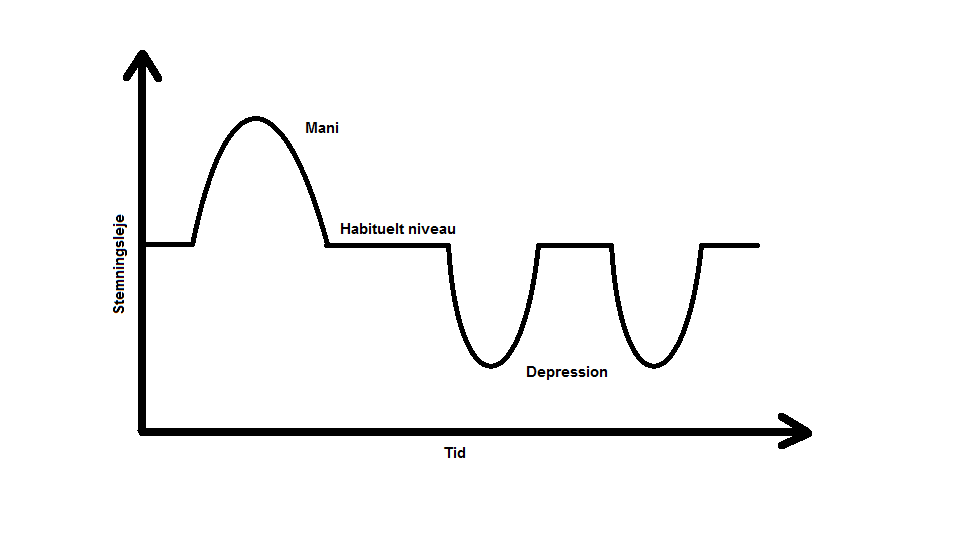
\includegraphics[scale=0.5]{affektivstemningsleje}
	\caption{Graf over stemningsleje for en patient med en mani og to depressions perioder.}\label{fig:stemningslejegrafeksempel}
\end{figure}

Det oftest sete er en mani episode og flere depressions episoder, men andre scenarier kan også forekomme.
Det gælder således om at have patienten på det habituelle niveau og hurtigt opdage når en patient afviger fra dette.

\input{indhold/moedemedjanne2}
\section{Møde med Psykiatri Professor Jørgen Aagaard}\label{sec:moede-med-joergen}
Denne sektion opsummerer et møde med psykiatri professor Jørgen Aagaard på Psykiatrien ved Sygehus Syd i Aalborg \citep{misc:jorgen-aagaard}. 
Jørgen er psykiater, samt almindelig somatisk læge, hvor hans fokus område er primært forskning ind i psykiatriske sygedomme.
De detaljer fra mødet der er vigtige vil blive inkluderet i denne sektion.
\ivan{Prøv at finde en mere diplomatisk formulering}


Det mest vigtige for at kunne detektere optrapning eller nedtrapning af depression/mani er ændring i adfærd som f.eks. døgnrytme og generelt aktivitetsniveau. 
Det kan også måles på kropslig stress, hvilket kan være at patienten begynder at svede eller pulsen ændrer sig uden at lave noget aktivt. 
Det er selvfølgelig vigtigt for alle personer at de har en regulær døgnrytme eller et stabilt aktivitetsniveau, men det er mere vigtigt for deprimerede.

\paragraph{Social adfærd og døgnrytme}
Social adfærd ændrer sig ved depression og mani.
Ved depression ændrer døgnrytmen sig, at den naturlige sammenhæng mellem følelser og hvad der siges mindskes og at aktiviteter nedsættes.
Ved mani er det lidt anderledes, de sover mindre, er mere urolige, har forskellig seksualitets niveau, de spiser mindre og at social kontakt gennem mobil kan være spam lignende. 

Hvis døgnrytme kan detekteres ved hjælp af en mobil kan ændringer i denne detekteres, hvilket er vigtigt da hvis man ved at døgnrytmen er ved at ændrer sig ved man at lidelsen er ved at ændrer sig.

Såfremt det er muligt at måle social eller fysisk aktivitet på telefonen, kan dette bruges til at måle ændringer hvilket kan indikere en ændring i lidelsen.

På samme tid hvis man kan måle kropslig stress kan dette også indikere en forværring af lidelsen, dette kunne f.eks. være måling af rystelser, sved eller puls. 

Det der er mest værdifuldt er at registrere døgnrytme, altså hvornår man går i seng og hvornår man står op, og på samme tid også se på om man kan registrere forstyrret søvn hvor patienten vågner i REM søvn. 
Det er også vigtigt at registrere social aktivitet, og måske at kunne registrere kropslig stress.

\paragraph{Ændringer}
Jørgen lagde meget stor vægt på at der ikke kan dannes et generelt billede af hvordan adfærd ser ud for en rask person som man derefter kan sammenligne med for at finde ud af om en person har enten depression eller mani.
Det er derfor nødvendigt at finde en baseline for individet og derefter kigge på ændringer i forhold til denne baseline.

\paragraph{Kognitive ændringer}
Hvis man er stresset vil man få det værre. 
Kognitive egenskaber som korttidshukommelse og løsning af matematiske eller logiske problemer vil være hæmmet.
Man kan derfor forestille sig at patienten skal udføre en test der afprøver patientens evner i disse områder.

\paragraph{Visuel repræsentation}
Hvis man skal præsentere tilstanden for patient skal den være enkel og være på patientens egne præmisser. Det er en god idé at præsentere hvordan patienten har det ud fra den registrering applikationen har gjort. Dette skal så kunne bruges som et hjælpemiddel der kan give objektiv information til patienten om deres tilstand.

Det komplette referat af mødet med Jørgen Aagaard, se \cref{app:moede-med-joergen-referat}.
\section{Fokusgruppe Interview}
Herunder vil blive beskrevet, samt reflekteret over, de vigtigste punkter fra interviewet.
For et komplet referat af fokusgruppe mødet, se \cref{app:fokusgruppe-interview-referat}.
Det bør her dog nævnes, at gruppen fik det indtryk at patienterne til mødet kun var unipolare og ingen officielle oplysninger blev givet om deres tilstand.

\subsection{Søvn}
Søvn er en vigtig faktor, hvilket alle deltagende var enige om.
Ikke blot varigheden af den daglige søvn, men også tidspunkt og kvalitet af søvn (fx. sammenhæng og rolig/urolig).
To af patienterne nævnte søvn som symptomer der, når set tilbage på, opstod en klar ændring i op til deres depressions-periode.
Andet interessant der blev nævnt her, var at der i forsøget på at falde i søvn blev udført beroligende aktiviteter såsom at se fjernsyn, læse eller drikke te.

\subsection{Social Tilbagetrækning}
Den sociale faktor blev der lagt mindre vægt på, dog var der enighed om at patienternes netværk, og kontakt til andre, mindskes under depressionen.
Social kontakt blev også benævnt som en god forebyggende handling, inden depression opstod.

\subsection{Early Warning}
(Også benævnt som intervention.)
Dette var oprindeligt antaget som en usikker, og til dels farlig, feature.
Der var dog enighed om at det kunne være godt at blive gjort opmærksom på, i god tid, at ens situation er under forværring.
Der bliver dog nødt til at gøres overvejelser omkring levering og formulering af sådanne notifikationer.
Det bør i højere grad knyttes til ændring i adfærd, frem for advarsel om at depression var på vej.
Der var også stor enighed om at det kunne være godt at blive gjort opmærksom på at søge hjælp, enten ved læge (forbundet med medicin) eller ved hjem og venner.

Ved tidlig advarsel kunne patienterne også gribe til deres forebyggende handlinger, her blev nævnt motion og strukturering af hverdag 
(Tidligere nævnte Janne lystbetonede aktiviteter).

\subsection{Dagbog og Status}
Ligesom interventioner, var det tidligere antaget at direkte input fra brugere var en dårlig ting.
Dette var dog ikke set som en dårlig ting fra patienterne, som var interesseret i hvad som helst som kunne hjælpe dem med at undgå depression.
Dette kunne både være en dagbog der skal skrives hver dag, eller løbende status-opdatering (fx. ift. nuværende tilstand).

En vigtig ting er dog at disse ting foregår inden depression, da under depression vil sådanne ting synes uoverkommelige set fra patienten synspunkt.

\subsection{Tilpasning i forhold til Symptomer}
Som forventet, så er der forskel på de individuelle symptomer.
Både hvilke ting der skal holdes øje med (fx. søvn) og på hvilken måde disse fremtræder (fx. kvalitet og længde af søvn samt tidspunkt for søvn).

I forhold til tilstands-spørgsmål skulle disse kunne vælges til/fra, samt tilpasses.


\section{Vigtige begreber}
Dette afsnit definerer vigtige begreber inden for psykiatrien, som patient empowerment, trends, cykler og interventioner.

\subsection{Patient empowerment}\label{sec:patientempowerment}
Patient empowerment omhandler en inddragelse af patienten i egen behandling.
Dette inkluderer at give redskaber til patienten, der gør det nemmere for patienten at vurdere sin egen sygdomssituation og foretage informerede behandlingsvalg ud fra den vurderede sygdomssituation.
Det er noget sygehusvæsenet gør en indsats for at implementere \citep{misc:patientpowerhovedstaden}.
Dog er det vigtigt at patient empowerment udføres ordenligt.
Steder hvor strategien ikke er at foretrække, er hvis patienten føler sig utryg ved at skulle have et sådant ansvar for egen behandling og patienten helst ikke vil indrages yderligere i behandlingen.
Derudover kræver det at patienten bliver velinformeret om hvordan han skal monitorere egen sygdom og handle ud fra det.

Til at understøtte denne informering af patienten om egen sygdom kan diverse empiri kilder være fordelagtige, såsom søvnændringer og aktivitetsændringer (se evt. \cref{sec:moede-med-joergen}), og er derfor undersøgt nærmere i dette projekt.
Måder man kan understøtte denne selvbehandling er ved at se på diverse mønstre og handlinger, hvilket inkluderer trends, cykler og interventioner.

\subsection{Trends}
Trends beskriver tendenser i en persons adfærd, eksempelvis at man går i seng kl. 22 og står op kl. 7 eller går en tur hver aften.
Det interessante med trends er at se på ændringer, da disse kan antyde en ændret sindstilstand.
En ændring kunne være at personen i en periode går i seng kl 4 i stedet for kl. 22, eller sover til kl 12 i stedet for kl. 7.

\subsection{Cykler}
Cykler omhandler fænomenet at en persons sindstilstand går i cirkler.
Dette er interessant da ens adfærd bliver påvirket af ens sindstilstand.
Ved at kunne detektere den nuværende sindstilstand og have kortlagt cyklus for den pågældende person, kan dette bruges til at forudsige det næste stadie, der kunne være en depression.

\subsection{Interventioner}
Interventioner omhandler handlinger der kan afbryde en periode eller påbegyndende periode.
Her menes periode som en tidsperiode med drastisk ændret stemningsleje, som ved depression eller mani.
Eksempelvis ved en påbegyndende depression, kunne man bryde ud fra sit nuværende mønster og i stedet foretage sig en lystbetonet aktivitet.


\section{Eksisterende systemer}
Der eksisterer allerede systemer, som implementerer mange af de ting, der er tiltænkt dette projekt eller har lignende funktionalitet, såsom fitness applikationer. 
Systemerne, der undersøges og beskrives er Ginger.io, Apple Health, Google Fit, Microsoft Health og Healthvault.

\subsection{Ginger.io}
Ginger.io er en applikation til iPhone og Android, beregnet til at assistere patienter med diverse psykiske lidelser \citep{ginger_dot_io,gingerio_mit,gingerio_dailymail}.

Applikationen er lavet til at assistere i behandlingen for følgende lidelser: depression, angst, bipolær affektiv lidelse og skizofreni.

Efter at applikationen er installeret, vil den indsamle data, de data kan så bruges til at sige noget om mobil-brugerens sindstilstand.
Der bliver overordnet set indsamlet to typer data; aktiv og passiv.
Aktiv data er forespørgsler fra applikationen, hvor mobil-brugeren selv skal svare.
Passiv data indsamles i baggrunden, og består af interaktions- og lokations-data, hvor interaktions-data er mobil-brugerens opkald- og SMS-vaner og lokations-data er opfanget via GPS og accelerometer, for at sige noget om hvor og hvordan mobil-brugeren bevæger og opholder sig.

For at komme i gang med applikationen, skal brugeren indtaste relevant information, såsom diagnoser, behandlingsforløb og behandler.
Ud fra disse informationer vil applikationen tilpasse forespørgslerne brugt til indsamling af aktive data.
Derudover vil passiv data, der indsamles i de første dage bruges til at angive brugerens normal-tilstand.
Herefter vil brugeren modtage notifikationer om ændring i social eller fysisk aktivitet, og i værste tilfælde vil behandler eller anden angivet kontaktperson blive notificeret.

Brugere af Ginger.io skal være forbundet gennem en behandler, og denne behandler vil til enhver tid have adgang til alle brugerens informationer.
Den overordnede idé er at Ginger.io skal assistere behandlingsprocessen, ved at give en indikator på brugerens tilstand mellem klinikbesøg. 
Et eksempel på denne indikator kan ses i \cref{eksisterende_systemer:ginger_io_graf}.

\begin{figure}[h]
\centering
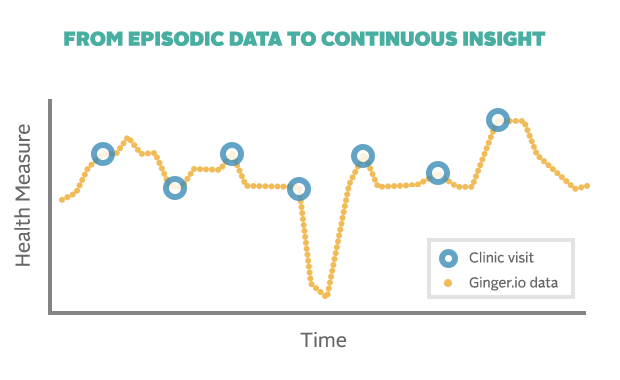
\includegraphics[width=.75\textwidth]{ginger_io_graph}
\caption{Figur fra https://ginger.io/for-providers/}
\label{eksisterende_systemer:ginger_io_graf}
\end{figure}

\subsubsection{Problemer}
Som det ser ud nu, er Ginger.io kun tilgængeligt i USA, og kun ved tilmeldte behandlere.
Derudover fungerer interaktions-data-indsamlingen kun på Android, hvilket betyder at iPhone applikationen kun indsamler data omkring lokation, samt aktiv data.

\subsection{Fitness trackere}
Der findes adskillige applikationer og større systemer til at styre ens fysiske aktivitet og velvære.
Heriblandt;
\begin{itemize}
\item Apple Health\citep{apple_health}
\item Google Fit\citep{google_fit,google_fit_api}
\item Microsoft Health\citep{ms_health} og HealthVault\citep{ms_health_vault,ms_health_vault_api}
\end{itemize}

Ens for disse fitness trackere, i modsætning til enkelte applikationer, er at de samler informationer fra et væld af forbundne enheder og applikationer.
Ydermere kan de indstilles til bestemte mål, og derved løbende fortælle om hvordan det går med at opnå disse mål.

\subsubsection{Apple Health}
Med Apple Health er det muligt at indsamle information fra andre applikationer (eksempelvis måltider eller hjertefrekvens), for at samle al data ét sted på sin mobil, eller synkronisere det med en iCloud konto.
Derudover er det muligt for andre applikationer at få adgang til Apple Health's data, ved at give tilladelse til forskellige kategorier af data.
Skærmbilleder af henholdsvis den oversigt Apple Health kan give, samt de kategorier der indsamles i, kan ses på \cref{eksisterende_systemer:apple_health_ss}.

\begin{figure}
\centering
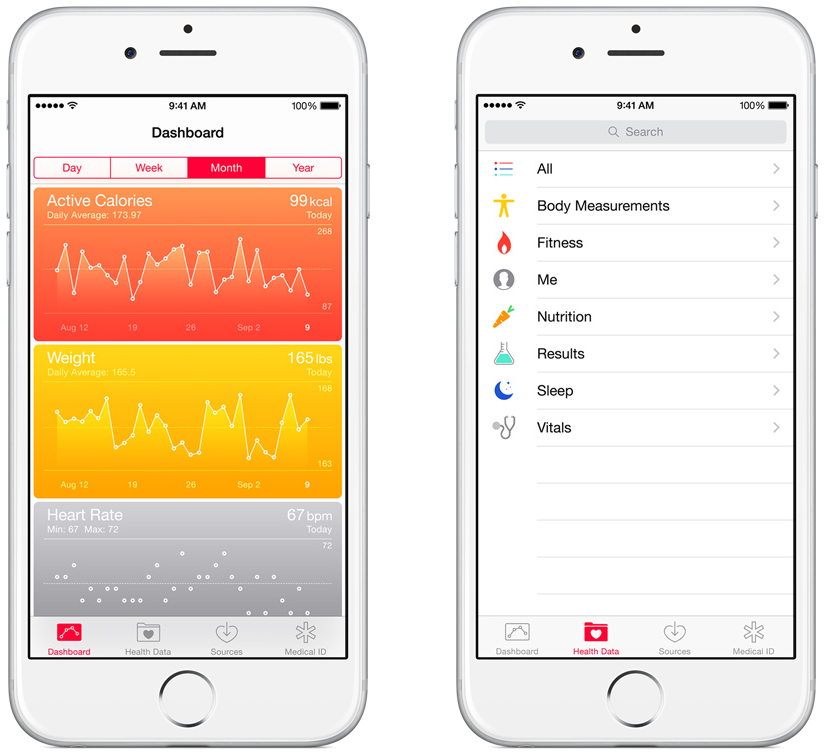
\includegraphics[width=.75\textwidth]{apple_health_ss}
\caption{Skærmbilleder af Apple Health fra \url{https://www.apple.com/ios/whats-new/health/}}
\label{eksisterende_systemer:apple_health_ss}
\end{figure}

\subsubsection{Google Fit}
Ligesom Apple Health, kan Google Fit samle data fra andre applikationer.
Derudover kan Google Fit også indsamle data fra andre kilder, såsom wearables.
Derefter er det muligt at få oversigt over ens aktiviteter og fysiske tilstand, via Googles egen side eller applikation.
Det er også muligt at lave sine egne applikationer, til både indsamling og visualisering, via Google Fit API (Android SDK eller REST web service).

Uden eksterne wearables eller applikationer, indsamles der kun bevægelses-data fra fx. GPS, hvor Google Fit applikationen selv estimerer om man går, løber eller cykler.
For andet aktivitet skal man manuelt indtaste (for eksempel roning eller yoga) sammen med varigheden.

Google Fit består af 4 komponenter:

\begin{description}
\item[Fitness store] er hvor de indsamlede data er gemt.
\item[Sensor framework] indeholder alt der skal bruges for at indsamle og repræsentere data, gennem repræsentationerne: \textit{Data Sources, Data Types, Data Points, Datasets, Sessions}.
\item[Permissions and User Controls] styrer adgang til de 3 data-kategorier: \textit{activity, location, body}.
Der gives læse eller læse+skrive rettigheder til én eller flere kategorier.
\item[Google Fit APIs] dækker over Android SDK og REST web service.
\end{description}

\subsubsection{Microsoft Health og HealthVault}
Microsoft Health er det overordnede system, som kan ses på \cref{eksisterende_systemer:ms_health_fig}.
HealthVault er hvor de indsamlede data er samlet og gjort tilgængelig for andre applikationer, via en web service.
Applikationer der vil gøre brug af HealthVault skal anmode om specifikke rettigheder (såsom til allergi-informationer eller mad-indtag).
I skrivende stund er der kun SDK til .NET framework.

Ud over at indsamle data fra smart devices og wearables, kan man i HealthVault også uploade dokumenter såsom røntgenbilleder.
Idéen er at man skal samle alle helbreds oplysninger ét sted, ikke kun dem vedrørende fitness.

Der er 4 vigtige koncepter i HealthVault:
\begin{description}
\item[Record] er medicin og fitness information for en enkelt person.
\item[Person] er et individ, som har fuld adgang til sin egen \textbf{Record}, med mulighed for at få adgang til andre personers records.
\item[Thing] er noget bestemt data gemt i en \textbf{Record}.
\item[Thing type] er typen for en \textbf{Thing}, hvilket beskriver hvad det er for en måling (såsom vægt eller blodtryk).
\end{description}

\begin{figure}
\centering
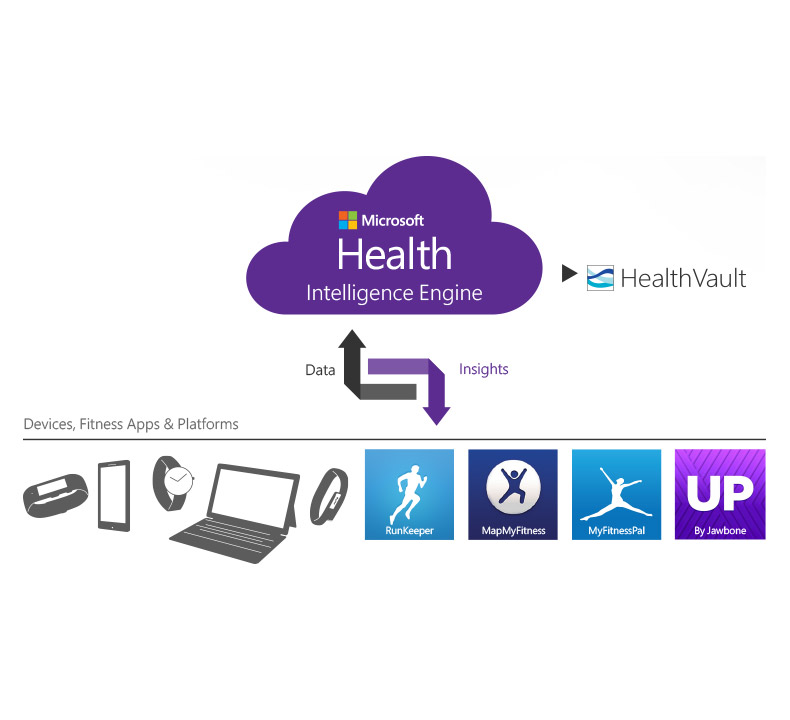
\includegraphics[width=\textwidth]{ms_health}
\caption{Microsoft Health fra \url{http://www.microsoft.com/microsoft-health/en-us}}
\label{eksisterende_systemer:ms_health_fig}
\end{figure}

\subsubsection{Problemer}
Disse forskellige systemet har problemer, som også skal overvejes.

\paragraph{Apple Health}
Apple Health er naturligvis lukket til iOS, hvilket gør at det kun er Apple produkter der kan tilsluttes til Apple Health.
Som det er nu, er det ikke muligt at dele helbredsoplysninger direkte med andre personer.

\paragraph{Google Fit}
Ifølge Google Fit Terms and Conditions er det ikke tilladt at bruge Google Fit til andet end fitness-formål, for eksempel at gemme lægelige eller biometriske data.\footnote{''Do not use Google Fit APIs for non-fitness purposes, such as storing medical or biometric data, selling data, or using data for advertising.''}
Lægelige data dækker over lægefaglige data, såsom diagnoser og sygdomsforløb.
Biometrisk data dækker over data, som kan identificere en person, såsom iris-skan eller stemmemønster.

\paragraph{Microsoft Health og HealthVault}
Ved brug af Microsoft Health er det kun muligt at hente data ned, efter det er i skyen.
Det vil sige at det ikke er muligt at få fat i rå data, som ved Google Fit.
På nuværende tidspunkt er der ingen SDK'er til Microsoft Health, det er kun muligt at få adgang til data via web service'en.

\section{Valg af Platform}\label{sec:valg_af_android}
Platformen for projektet skal vælges, her ses der på hvilke fordele og ulemper de forskellige platforme har og endeligt laves der en beslutning.

Der er forskellige platforme der kan vælges, specifikt Android, iPhone og Windows Phone.
Der kunne også vælges en hybrid platform som for eksempel Apache Cordova der tillader udvikling af smartphone applikationer ved hjælp af HTML, CSS og JavaScript \citep{misc:apachecordova}, eller kryds platform udvikling som for eksempel Xamarin der tillader udvikling i C\# som kan kompileres til mange forskellige operativ systemet såsom Android, iOS og andre \citep{misc:xamarin}.

Fordelene ved Android er som følgende:
\begin{itemize}
\item Det er en meget åben platform som giver adgang til meget sensor data
\item Android har flere brugere end iPhone og Windows Phone.
\item Der er ingen begrænsninger på hvad der kan udvikles
\item Der er mange udviklings ressourcer tilgængelige såsom guides, tutorials.
\item Android applikationer udvikles som regel i Java, hvilket er et udbredt programmeringssprog.
\end{itemize}

Android har dog også ulemper, såsom mange forskellige typer smartphones med forskellig hardware og forskellige versioner af operativ systemet.

Fordelene ved iPhone er primært at der er nemmere at udvikle til da det ikke er særlig fragmenteret i forhold til Android. 
Brugerfladen er meget standardiseret hvilket gør det nemmere at udvikle den del af applikationen. 
iPhone har ulemper, da det er et meget mere lukket system hvilket gør at data kan være umulige at få fat i. iPhone udvikling foregår kun på OS X, og kræver en licens. iPhone udvikling foregår i et sprog som ikke bruges bredt, Objective-C.

Fordelene ved Windows Phone er et meget modent/godt udviklingsmiljø og programmeringssprog, og at brugerflade design er meget nemt. 
Ulemper ved Windows Phone er så at der ikke er særlig mange udviklings ressourcer tilgængelig da Windows Phone markedet ikke er særlig bredt. Windows Phone er også en lukket platform.

Fordelene ved en hybrid platform som for eksempel Apache Cordova er at ens applikation kommer ud til den bredest mulige målgruppe, da man her har adgang til alle de forskellige smartphone enheder.
Det muliggøre at skrive en applikation i HTML, CSS og JavaScript og gør det muligt at lave en applikation uden at bruge platformens native codelanguage.
Et problem med cross platform er komplicerer designprocessen, da hver smartphone platform har forskellige design guidelines.
Derudover giver det også en væsentlig uoverensstemmelse mellem hvad man kan forvente af de underliggende datalag, hvilket kan gå ud over kvaliteten af det udviklede software.

Vores projekt er meget afhængig af åben adgang til datakilder, hvilket Android giver bedre adgang til.
Vores situation er også at udvikling på Android virker nemmere da det ikke påkræver et specielt operativ system da ingen på udviklingsholdet har OS X computere, og at udvikling i Java er kendt blandt mange på udviklingsholdet.
Desuden fravælger vi også hybrid- og kryds platform, idet at brug af disse vil have den konsekvens at lav-niveau kontrol vil blive tabt og at verificering af systemet vil kræve flere telefoner at teste på.



\chapter{Essence}
For at danne et bedre overblik over projekt, problem og løsning er der brugt en række teknikker som er stillet til rådighed i Essence \cite{art:essence}.
Dette udkast af Essence er brugt i forbindelse med undervisningen i kurset Software Innovation på Aalborg Universitet, under bogens forfatter Ivan Aaen.
Dette kapitel vil tage udgangspunkt i de 4 \textit{views} fra Essence; \textit{Paradigm, Product, Project og Process}.
Der er dog lagt vægt på de elementer som knytter sig til problem og overordnet idé, da produkt i større detalje vil blive præsenteret senere.

% Systematisk beskrivelse af konfigurations tabel.
\section{Konfigurationstabel}
En konfiguration af et system er en kombination af elementer, og en konfigurationstabel beskriver den konfiguration.

Denne beskrivelse er baseret på  \citet[Afsnit 3.2]{art:essence}.

Systemets `use context' er at systemet bruges til at informere unipolare og bipolare patienter om der har været åbenbare adfærdsændringer. Udfordringen er så om mobilen kan bruges til at gøre dette ved hjælp af sensorer på mobilen.

Den øverste række i \cref{tab:konfigurationsTabel} navngiver de fire Views i Essence: Paradigm, Product, Project og Process.

`Focus' rækken repræsenterer de største problemer og løsninger i projektet. 
Udfordringen er tiltænkt til at være om man kan bruge en mobil til at overvåge adfærd af unipolare og bipolare patienter og gøre dem opmærksom på adfærdsændringer og dette er så tiltænkt at disse patienter åbner en applikation på denne mobil hvor de vil blive blive givet et overblik og derved få at vide om der har været adfærdsændringer. 
Det er så vigtigt at systemet skal kun observere og informere og derved bruge konceptet 'patient empowerment'.
Løsnings strategien er så at bruge en smartphone, og udvikle et system som kan registrere data fra forskellige sensor moduler og gemme det på telefonen som den bliver brugt af patienten.
Data den indsamler skal være objektiv, så idéen er at den skal fungere som en objektiv dagbog.
Denne data kan så bruges til analyse og blive undersøgt om der er nogle ændringer i patientens opførsel og skal let kunne aflæses af patienten hvorfra de kan få relevant information fra den præsenterede data. 

`Overview' rækken repræsenterer projektets stakeholders. Hoved perspektivet er selvfølgelig fra patienterne, da det er dem som skal bruge produktet men der er også sponsorer som er interesseret i at se projektet være en succes da det vil gøre at deres patienter vil få det nemmere. 
Designet på projektet er simpelt idet at der bruges mobil eller wearables til sensor input og at denne data gemmes og analyseres på mobilen. 
For at evaluere denne funktionalitet kan der bruges fokusgrupper og usability tests til at finde ud af om den er akkurat, let-tilgængelig og forståelig.
Argumentet for at lave et sådant projekt er, at depression og mani ofte opdages for sent, hvilket i det fleste tilfælde gør situationen værre.
Hvis symptomerne identificeres så perioden opdages tidligt kan den måske forhindres, hvilket kan spare staten en del udgifter til behandlinger og indlæggelser.
Der er dog det problem at en smartphone baseret løsning som der her sigtes efter selvfølgelig kræver en smartphone, og også stiller lidt krav til at folk kan bruge deres smartphone.
Dette er dog bare et minimalt problem da en stor del at befolkningen har smartphone nu om dage så derfor kan man også gå ud fra de kan finde ud af at bruge den på et acceptabelt niveau.
Selv hvis en potentiel bruger ikke har en smartphone, koster den lettilgængelige teknologi ikke så meget, så at investere i den som et behandlingsmiddel er en reel mulighed.

`Details' rækken repræsenterer nøgle scenarier, nøgle componenter og features.
Desuden indeholder det sidste felt i denne række også de findings.
Findings er dog en speciel i forhold til resten af tabellen, da findings ikke kan sættes i tabellen til at starte med, hvilket jo også lidt ligger i navnet.
Findings kommer som et resultat af at have arbejdet med udviklingen af det system resten af konfigurationstabellen beskriver og under evalueringen af dette. 
Det vi har fundet ud af er at der kunne være potentielle problemer med pladsforbrug, med batteriforbrug, at der kan være huller i data og at der kan være problemer med persondataloven som vi ikke har undersøgt.

\begin{figure}
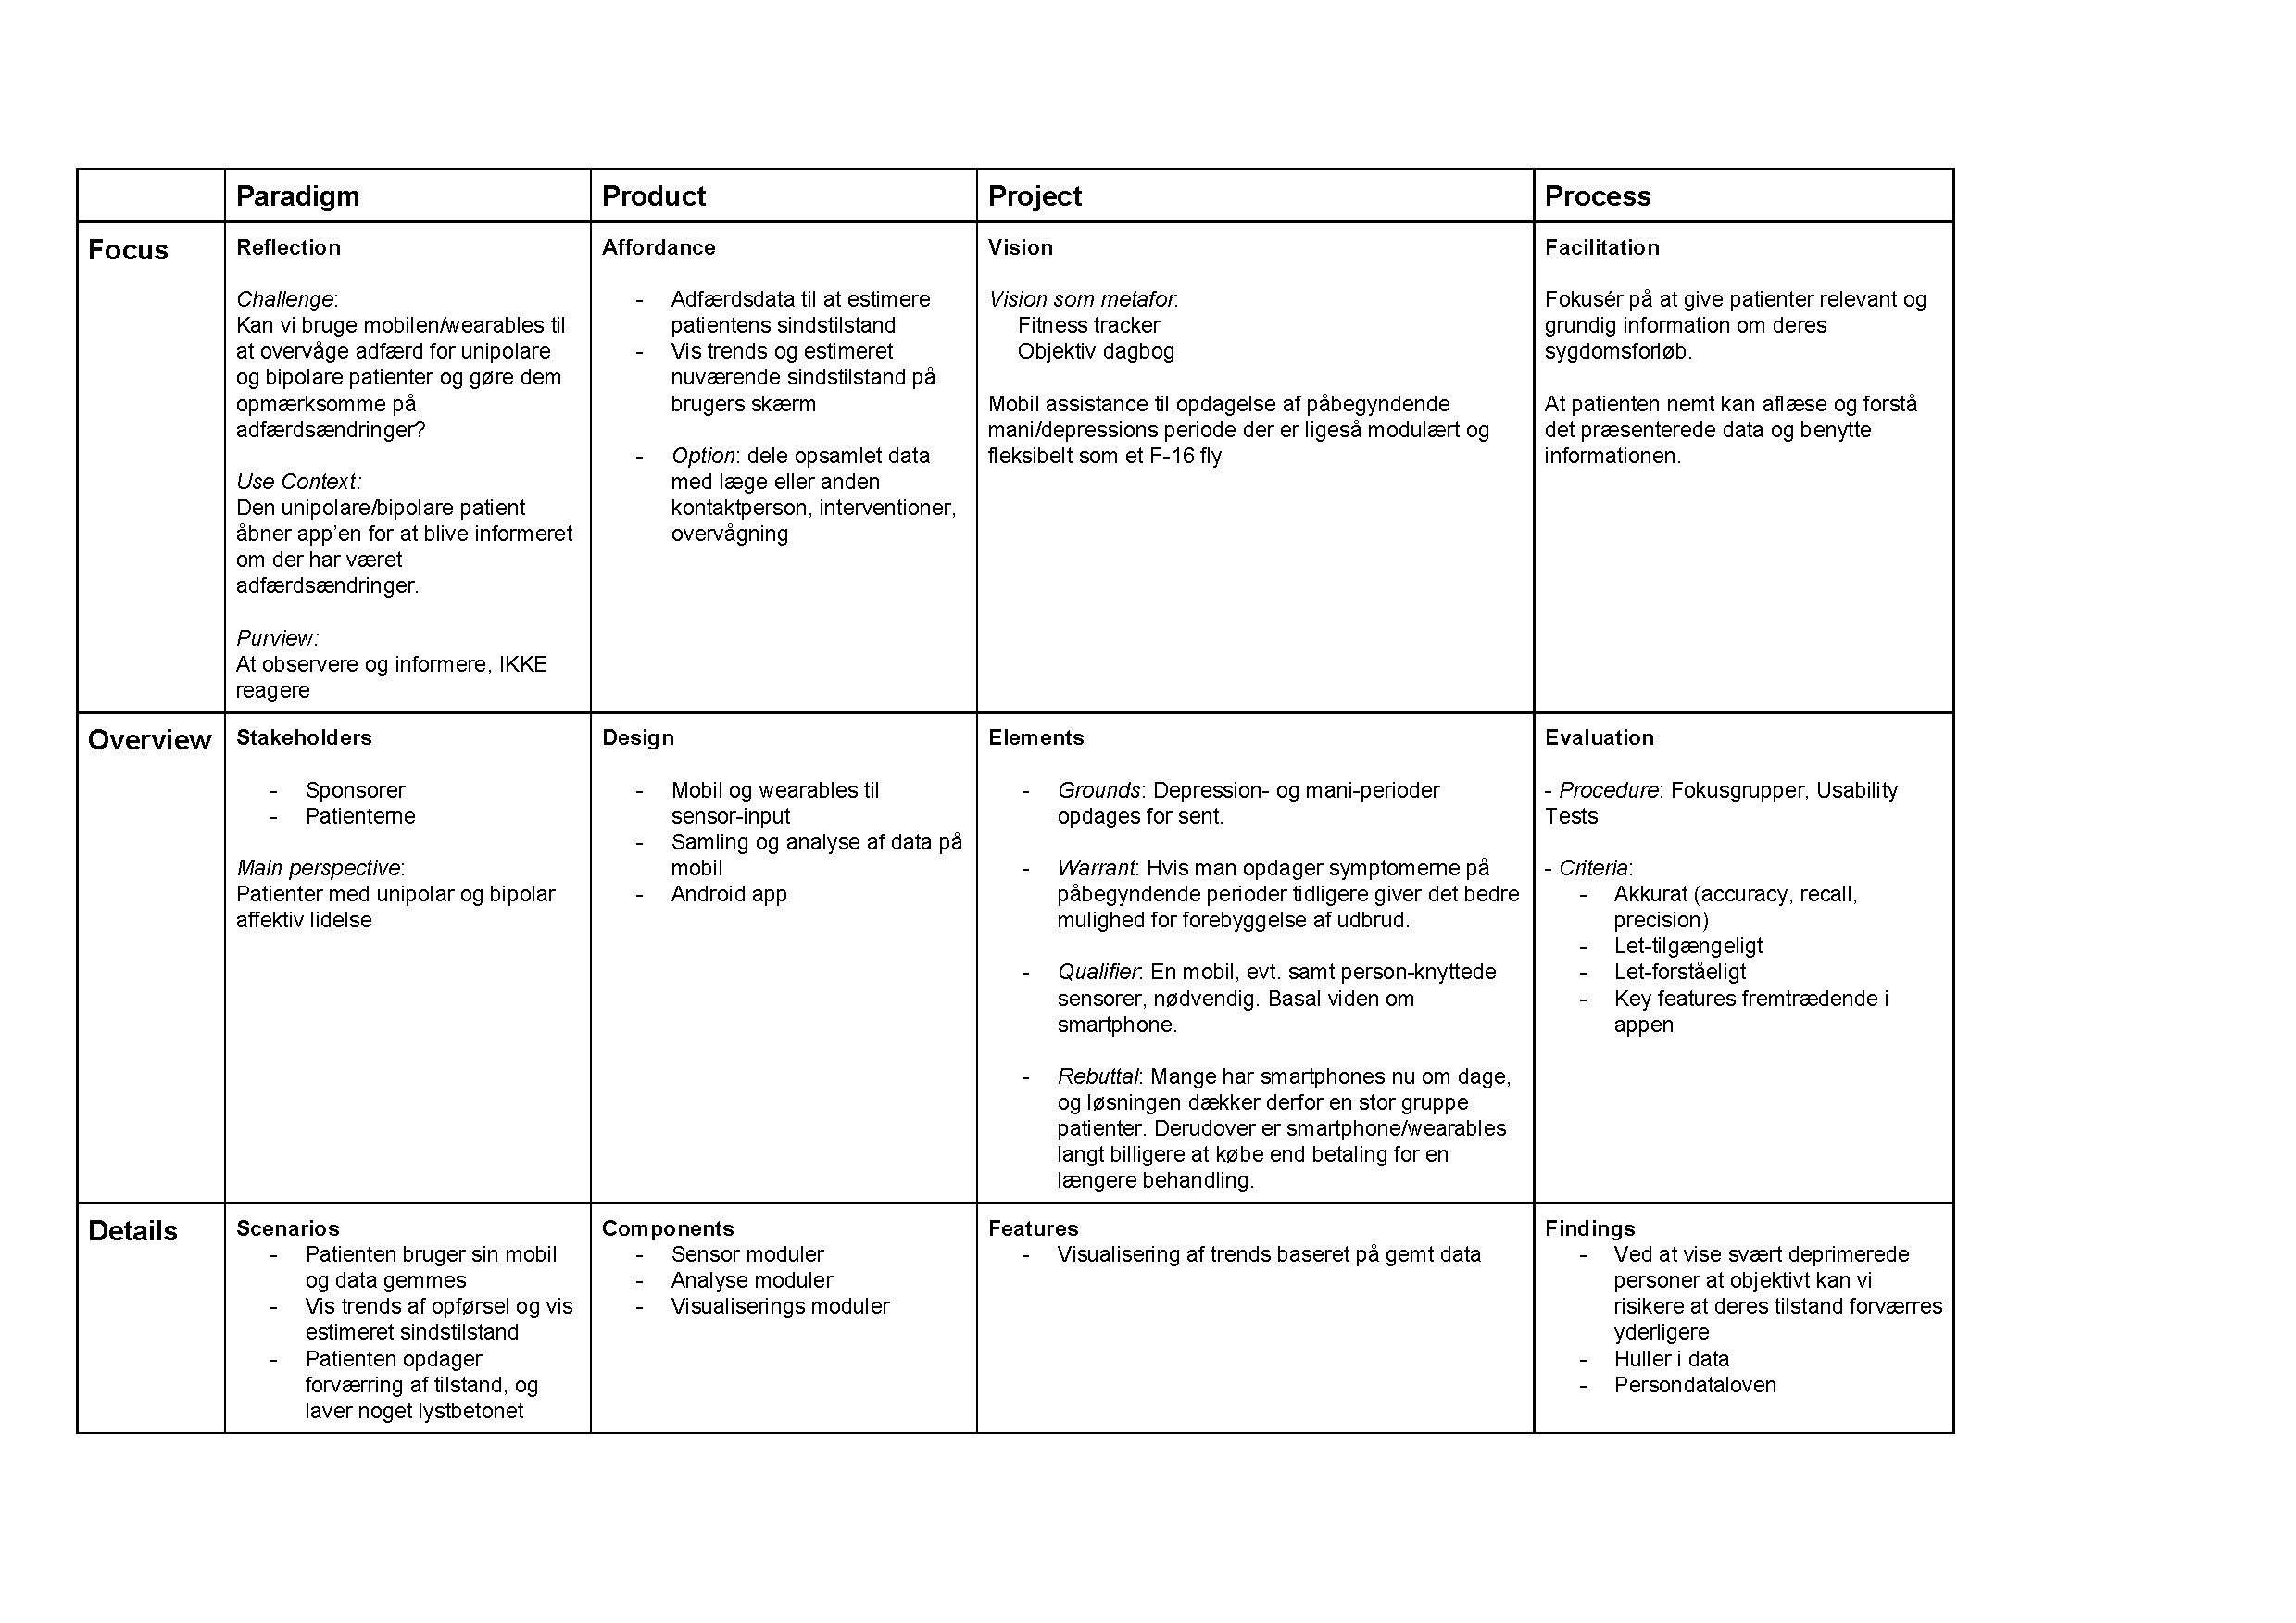
\includegraphics[scale = 0.65,trim = 1cm 3cm 6cm 2cm, angle = 90, clip]{KonfigurationTabel}
\caption{Konfigurations tabellen for systemet.}
\label{tab:konfigurationsTabel}
\end{figure}

\section{Vision}
For at få et 'Vision' af projektet overvejes der følgende koncepter fra \citet{art:essence}, derudover er der enkelte oversatte citater derfra.
\textit{Metafor}, \textit{Ikon}, \textit{Prototype} og \textit{Proposition} er de forskellige muligheder som bogen præsenterer som kan bruges til at repræsenterer en vision.

Ifølge bogen er Metafor \textit{et ord eller sætning der repræsenterer eller figurativt beskriver en løsning uden af være bogstavelig anvendelig.}
Bogen beskriver Ikon som \textit{et symbol der eksemplificerer en eller flere nøgle kvaliteter i en idé.} Det går på de visuelle, hvor øvelsen er hvordan man konkretiserer en eller flere nøglekvaliteter af en idé. Dette er eksempelvis hvor den teknologiske del er nemt udførlig, men hvordan det æstetiske i en løsning ikke er umiddelbar.
Derudover beskrives Prototype som \textit{en kompleks og konkret repræsentation af et vision. Prototyper er ufærdiggjort software som traditionelt bruges til at bekræfte udviklernes opfattelse af krav.} Denne bruges til at få feedback på en ufuldstændig software løsning, og er en fysisk repræsentation af løsning. 
Til sidst Proposition er \textit{er et udsagn som er velbegrundet og har positive egenskaber.} Denne svarer basalt set til en traditionel problemformulering. 

Vores vision for projektet repræsenteres ved hjælp af metafor repræsentationen, specifikt formuleres det ved hjælp af tre metaforer.
Vi bruger metafor på baggrund af at det giver et løst overblik over selve løsningen som giver plads til at ændre på løsningen uden at miste overblikket. 

De tre metaforer er \textit{Objektiv dagbog}, \textit{Fitness tracker} og \textit{F16 fly}.
At formulere vores vision som en metafor lader os koncist specificere hvad der er nøgleaspekterne af produktet.

Den objektive dagbog danner tanken om en dagbog baseret på objektive datakilder, hvilket svarer til sensor data, brugsdata etc.
Alt sammen data der kan indsamles uden brugerinteraktion.

Fitness trackeren som metafor planter tanken om en applikation der løbende evaluerer ens præstationsevne, hvilket kan oversættes til mentalt helbred.

F16 fly metaforen henvender sig til platforms designet, der er tiltænkt at være en meget modulær og kraftig platform, ligesom det er tilfældet med F16 flyet hvor man kan hægte en lang række komponenter på alt efter hvad der er brug for i den pågældende situation.
%\section{Udløsning af Projektet}
% Essence chapter 4.
Det er vigtigt at vide hvad der udløste projektet, altså hvad motiverede projektet. 
Det kan f.eks. være at der var et bruger behov for det, at en teknologisk mulighed opdages, at der var en løsnings mulighed hvor man 'genbruger' en udviklet løsning i et andet domæne og konkurrence stress hvor man vil prøve at få en konkurrencemæssig fordel. 

Det der udløste vores projekt var `bruger behov'.
Grunden til det kan klassificeres som brugerbehov er, at en person der arbejder med problemområdet kom med ideen til dette projekt. 
Det behov der er i problemområdet ligger i at personer med affektive lidelser har brug for en mere moderne tilgang til tilstands overvågning end et ugentlig møde med et psykolog der i løbet af denne periode skal finde ud af om de har det godt.

Det skal dog også siges at projektet har et kraftigt grundlag i 'teknologisk mulighed', da ideen til projektet er baseret på en teknologisk mulighed med smartphone som platform.
Denne mulighed er, at smartphones kan indsamle mange varierende datatyper, der muligvis kan bruges til at give et indblik i en persons sindstilstand.

\section{Kriterier}
Her vil de vigtigste kriterier, som skal opfyldes for at kunne kalde projektet en succes, blive præsenteret.
Disse kriterier dækker over to overordnede områder: i forhold til bruger, og i forhold til platformen i sig selv.

\subsection{Bruger}
\begin{description}[style=nextline]
	\item[Sikkerhed] 
		Eftersom systemet kan komme til at arbejde med person-følsomme data, er det vigtigt at denne data opbevares sikkert, så applikationer der ikke har lov til at se ens data ikke har mulighed for dette.
	\item[Stabilitet]
		For at sikre der ikke opstår for mange huller i den indsamlede data, skal systemet køre stabilt, så der kontinuert kan indsamles data.
	Hvis der opstår for mange huller, kan dette give et ufuldstændigt billede af patientens sindstilstand, som måske kan fejl-fortolkes.
	\item[Præcision]
		Ligesom ved huller i indsamlingen af data over tid, er det lige så vigtigt at data der kommer ind er præcis.
	Dette grundes at analyse på upræcis data vil give et upræcist billede af patientens sindstilstand, hvilket kan føre til fejlagtige vurderinger af denne.	
\end{description}

\subsection{Platform}
\begin{description}[style=nextline]
	\item[Fleksibilitet]
	Det skal være nemt at modificere funktionalitet til platformen, da platformen skal kunne tilpasses til forskellige individer.
	\item[Mulighed for udvidelse]
	Det skal være muligt at udvide platformens funktionalitet, uden at skulle ændre på selve platformen.
	Det skal gøres på sådan en måde at personer der ikke er en del af systemet, kan lave og tilføje egne dele til platformen.
	Dette giver naturligvis yderligere overvejelser ift. sikkerhed.
\end{description}

\subsection{Evaluering af kriterier}
For at evaluere de forskellige kriterier skal


\mikael{Hvordan skal vi evaluere på de kriterier? Hvad kunne være godt at gøre? Hvad har vi egentlig tænkt os at gøre?}
\bruno{Igen +1 til Mikael - damn it..}
\lasse{Mikael skriver dette, det sagde han at han ville d. 2015-05-19 kl 12:45}
\section{Paradigm view}
I dette view undersøges hvordan \textit{the Challenge} bliver set fra brugerens perspektiv.
Teknikker til denne undersøgelse inkluderer at definere applikationens problem domæne ved hjælp af en \textit{Use context} og \textit{Use Scenarios}.

\paragraph{Use context}

Fra konfig tabel:
Den unipolare/bipolare patient åbner app’en for at blive informeret om der har været adfærdsændringer.

\paragraph{Use Scenarios}

\chapter{Indsamling af Data}

Dette afsnit detaljerer hvilke kilder af data som kan bruges til dette projekt, hvilke devices der kan give adgang til de kilder, hvordan man logger på en mobil, pladsforbruget der kan forventes med platformen og hvordan kilder af data kan bruges.
\chapter{Indsamling af data}
Dette afsnit detaljerer hvilke kilder af data som kan bruges til dette projekt, hvilke devices der kan give adgang til de kilder, hvordan man logger på en mobil, og hvordan kilder af data kan bruges.
\section{Sensorer}
Dette afsnit beskriver de forskellige sensorer der findes og som kunne være interessant for projektet. 

\paragraph{Kamera}
Kameraet kan tage billeder og billedesekvenser i form af video optagelse.

\paragraph{Accelerometer}
Accelerometeret måler accelerationen i x,y,z retningerne i et koordinatsystem der er lagt på telefonen som vist på \cref{analyse:accelerometer:koo}.
Accelerometret kan konceptuelt forstås som en kugle der ruller rundt i et rum hvor væggene kan måle den kraft de bliver påvirket med.
På \cref{analyse:accelerometer:kraft} ses dette konceptuelle rum med påvirkning fra tyngdekraften. 
Sensoren vil i dette tilfælde rapportere en negativ kraft i z-aksens retning.

\begin{figure}[h]
	\centering
	\begin{subfigure}[b]{0.47\textwidth}
		\centering
		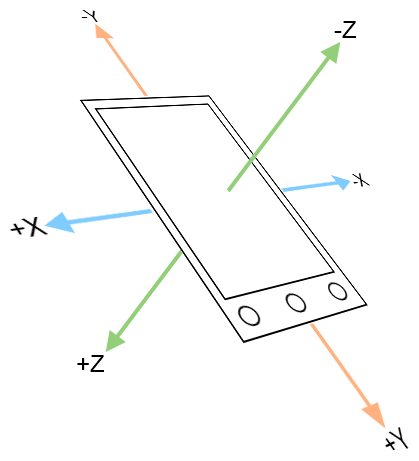
\includegraphics[width=.6\textwidth]{accelerometer-telefon}
		\caption{Koordinatsystem lagt på en telefon}
		\label{analyse:accelerometer:koo}
	\end{subfigure}
	~
	\begin{subfigure}[b]{0.47\textwidth}
		\centering
		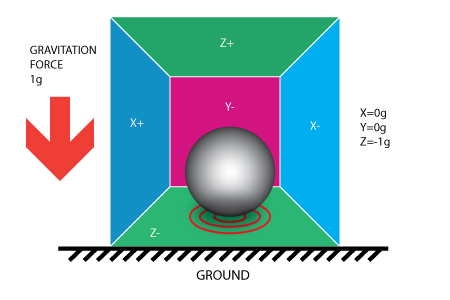
\includegraphics[width=\textwidth]{accelerometer}
		\caption{Konceptuel tegning af et accelerometers virkemåde. Illustration fra \citet{accelerometer}}
		\label{analyse:accelerometer:kraft}
	\end{subfigure}
	\caption{}
	\label{accelerometer}
\end{figure} 

\paragraph{GPS}
GPS sensoren giver en lokation som koordinater bestående af: breddegrad, længdegrad og en pejling.

\paragraph{Mikrofon}
Mikrofonen kan optage omgivelserne ved at konvertere akustisk lyd til elektriske signaler.

\paragraph{Lyssensor}
Lyssensoren kan måle lysniveauet i lux.

\paragraph{Pulsmåler}
Pulsmåleren måler pulsen i hjerteslag per minut.

\paragraph{Galvanisk Hud Respons}
Galvanisk hud respons sensoren giver adgang til data omkring hvor god hud er til at lede strøm, huden leder strøm bedre jo mere den sveder, og derfor giver det også data omkring hvor meget den sveder.
\section{Enheder}\label{sec:kilder-til-sensorer}
Dette afsnit beskriver de forskellige typer af enheder udstyret med sensorer, således disse enheder kan agere kilder til dataindsamling.

De overordnede typer af enheder er \textit{smartphones}, \textit{smart wristband} og \textit{smartwatches}. 

\paragraph{Smartphone}
er en generel platform til et meget bredt brug og har derfor typisk et væld af sensorer, som fx. GPS, accelerometer og gyroskop.
Disse bruges til forskellige funktioner i telefonen, både internt og eksternt, fx. kan gyroskopet bruges til at bestemme orienteringen af smartphonen, hvor GPS kan bruges til navigation.

\paragraph{Smart wristband} % Skal det hedde dette?
er et stykke udstyr som bruges til aktivitetssporing, primært af fitness og helbredsgrunde, hvor de bl.a. bruges til at måle aktivitetsniveau og søvnmønster.
Denne aktivitetssporing påkræver en mængde sensorer, disse kan være de sensorer der findes i smartphones, men også sensorer der måler direkte på kroppen, fx. sensorer der kan måle puls eller galvanisk hud respons. 
Dog varierer det meget hvilke sensorer der findes i de forskellige smart wristbands, afhængigt af prisklasse.
Et eksempel på dette kunne være en JawBone UP3 hvor man finder sensorer der måler temperaturen af omgivelserne og kroppen, puls og galvanisk hud respons \citep{misc:jawboneup3sensors}. 
Dette er i kontrast til andre smart wristbands hvor der f.eks. ikke kan findes en sensor til at måle galvanisk hud respons.

\paragraph{Smartwatch}
er en intelligent version af normale armbåndsure, i den forstand at et smartwatch giver ekstra funktionalitet som minder om det der findes i en smartphone \citep{msic:smartwatchstate}. 
Som eksempel på dette kan man spille spil på dem, læse SMS og bruge den som medie-fjernbetjening, dog er smartwatches mindre kraftfulde end smartphones. 
Smartwatches og wristbands har fordelen at det er noget man går rundt med og derfor har direkte kontakt til kroppen det meste af tiden.
Endvidere har smartwatches mange af de samme sensorer som en smartphone og et smart wristband, ofte har de ikke sensorer til kropslige målinger, hvor de så primært fungerer som en hybrid mellem en smartphone og et smart wristbands.

\subsection{Opsummering}
Smartphones er alsidige platforme der kan bruges til at køre applikationer.
De indbyggede sensorer gør dem til en attraktiv platform at udvikle på, men smart wristbands og smartwatches har mere specialiserede sensorer som bedre understøtter logning af relevant helbredsdata.
På baggrund af dette ses det at smartphones kan bruges til meget, men hvis man vil have kropslige målinger er det en god idé at enten bruge et smart wristband eller et smartwatch med de relevante sensorer.

I \cref{tab:sensorsInDevices} er der et overblik over hvilke sensorer der findes i de forskellige slags udstyr. * indikerer at de kan findes i den slags udstyr, men det er ikke særlig tit at man finder det.

\begin{table}[h]
\centering
\begin{tabular}{|c|c|c|c|}
\hline  			 & Smartphone 	& Smart wristbands 	& Smartwatch	 	\\ 
\hline Accelerometer &  \checkmark 	& \checkmark		& \checkmark  		\\ 
\hline Gyroskop		 &	\checkmark	& \checkmark		& \checkmark		\\
\hline Kompas		 &  \checkmark	&					& \checkmark		\\
\hline GPS			 &	\checkmark	&					& \checkmark*		\\
\hline Barometer	 &	\checkmark	&					& \checkmark		\\
\hline Rumtemperatur &				& \checkmark*		&					\\
\hline Hudtemperatur &				& \checkmark*		& \checkmark		\\
\hline Lyd			 &	\checkmark	&					& \checkmark		\\
\hline Lys			 &	\checkmark	& \checkmark*		&					\\
\hline Kamera		 &	\checkmark	&					& \checkmark*		\\
\hline Puls			 &				& \checkmark		& \checkmark*		\\
\hline GHR			 &				& \checkmark*		& \checkmark*		\\ \hline
\end{tabular}
\caption{Overblik over sensorer i forskellige platforme.}\label{tab:sensorsInDevices}
\end{table}

\section{Mobil logning}
Dette afsnit fortæller om de forskellige ting der er mulige at logge på telefonen, som er interessante for projektet.

\paragraph{Opkald}
Opkaldsoversigten i Android giver adgang til opkalds historikken.
Applikationer skal dog have adgang til dette.
Et opkald består af tidspunkt, modtager, afsender og varighed.

\paragraph{Applikationer}
Det er muligt at logge hvilke applikationer der bliver brugt ved at se hvornår applikationerne er aktive.

\paragraph{Skærm}
Android har events for hvornår en skærm tændes og slukkes.

\paragraph{Tastatur}
Logning af tastaturet er ikke muligt, da man ikke kan få adgang til det gennem en applikation.

\paragraph{SMS}
Det er muligt at få adgang til SMS beskeder, det kræver dog tilladelse fra brugeren til applikationen.
\section{Pladsforbrug eksperimenter}\label{eksperimenter}
Det faktum at der skal indsamles data kommer med den konsekvens at en mængde plads på smartphonen skal bruges.
På mobile enheder er der begrænset lagerplads, som eksempel har en Samsung Galaxy S4 enhed kun 16 GB hvorimod mange computere nu om dage har mindst 1 TB (ca 64 gange mere).
Pladsforbrug er nødvendigt at forholde sig til, da det sætter en begrænsning på hvad man kan tillade sig at gøre på mobile enheder.
I vores tilfælde skal det overvejes hvor stor en mængde data, der kan lagres og samtidig tillade brugen af andre applikationer på en persons smartphone.
For at undersøge hvordan de forskellige datakilder bruger pladsen på en smartphonen opstilles to eksperimenter.
Hvis pladsforbruget viser sig for stort skal data enten komprimeres, aggregeres eller man bør overveje muligheden for ekstern lagring.

Eksperimenterne blev udført på en Samsung Galaxy S4 hvor følgende datakilder blev lagret i den samme SQLite database:

\begin{itemize}
	\item Lyd - En datakilde der oplyser maks amplituden over en periode.
	\item Skærm - En datakilde der oplyser når skærmen slukkes og tændes.
	\item Nærhed - En datakilde der oplyser afstanden fra smartphonen.
	\item Placering - En datakilde der oplyser den nuværende placering.
	\item Gyroskop - En datakilde der oplyser den nuværende rotation.
	\item Accelerometer - En datakilde der oplyser den nuværende acceleration.
\end{itemize}

Dette udvalg er de datakilder der på eksperiment tidspunktet var vurderet som sandsynligvis værende relevante senere i udviklingsforløbet.
Det er vigtigt at bemærke at de ikke er i deres endelige form og at listen ikke er komplet.
Som platformen bliver udviklet kommer der flere datakilder og måske udelades nogle også.
Disse eksperimenter vil derfor kun kunne give et estimat for pladsforbruget.

Datakilder som Skærm, Nærhed og Placering producerer kun data når der sker ændringer. 
Derfor blev det første eksperiment udført på en måde, der efterligner en potentiel brugssituation. 
Smartphonen blev bevæget og skærmen blev tændt og slukket flere gange under testperioden.
Det første eksperiment blev udført over 30 minutter.

Det andet eksperiment blev udført over en weekend, hvor smartphonen lå stille.
Dette eksperiment burde vise et minimumsforbrug for datakilderne.

\paragraph{Forespørgselshastighed}
Pladsen som datakilder bruger vil naturligvis afhænge af hvor ofte datakilderne forespørger for data.

I Android er der forskellige metoder til at angive forespørgselshastigheden på en datakilde.
Der findes fire konstanter, der kan benyttes til at angive hastigheder der passer i forskellige kontekster \citep{sensormonitor}.

\begin{itemize}
	\item SENSOR\_DELAY\_FASTEST forespørger så hurtigt som muligt.
	\item SENSOR\_DELAY\_GAME forespørger hvert 20. ms, og er beregnet til spil.
	\item SENSOR\_DELAY\_UI forespørger hvert 60. ms og er tilstrækkeligt til brug i brugergrænseflader.
	\item SENSOR\_DELAY\_NORMAL forespørger hvert 200. ms er tilstrækkeligt til at opfange ændringer i skærm orientering.
\end{itemize}

Det er muligt at angive opdateringen i ticks hvis man vil have en langsommere opdatering.
Det skal bemærkes at disse angivelser kun benyttes som et hint til smartphonen, det kan ikke garanteres at data bliver forespurgt med det angivne interval.
I dette eksperiment er SENSOR\_DELAY\_NORMAL benyttet.

\subsection{Resultater}
Til analyse af pladsforbruget blev programmet \textit{SQLite-analyzer} benyttet \citep{sqliteanalyzer}.
SQLite-analyzer viser statistik for en SQLite database inklusiv data for de enkelte tabeller.

\paragraph{30 minutters eksperiment}
Efter 30 minutter fyldte databasen $1\,156\,459$ bytes ($\approx1.16$ MB).
Under antagelsen at datakilderne vil fortsætte med at generere data med den samme hastighed vil det efter 24 timer fylde omkring $\approx56$ MB. 

De enkelte datakilders var fordelt på følgende måde (sorteret efter pladsforbrug),

\begin{tabular}{|c|c|c|c|}
	\hline Datakilde		& Plads forbrug i bytes				& Antal datapunkter  & \% af databasen \\
	\hline Accelerometer 	& $609\,266$ B / $\approx609$ KB	& $12\,434$ 		 & $52.7$ \\ 
	\hline Gyroskop 		& $495\,018$ B / $\approx495$ KB	& $10\,146$ 		 & $42.8$\\ 
	\hline Lyd 				& $42\,648$ B / $\approx43$ KB		& $1\,706$ 			 & $3.3$ \\ 
	\hline Placering 		& $4\,751$ B / $\approx5$ KB		& $91$ 				 & $0.41$ \\ 
	\hline Nærhed    		& $3\,173$ B / $\approx3$ KB		& $135$ 			 & $0.27$ \\ 
	\hline Skærm 			& $1\,242$ B / $\approx1$	KB		& $54$				 & $0.11$ \\ 
	\hline 
\end{tabular} 

Som det ses af tabellen er de store pladssyndere `Accelerometer' og `Gyroskop' datakilderne.
Dette skyldes at de forespørger meget ofte og gemmer al data.

Lyd datakilden gemmer kun maks amplituden over en periode af 1000ms, af denne grund fylder dens data ikke mere end 3.3\% af databasen.
Afhængig af hvad man vil analysere vil det være nødvendigt at gemme væsentligt mere end dette.

Placerings datakilden forespørger kun når der er en tilstrækkelig ændring i placeringen.

Nærhed datakilden ændrer sig kun når man sætter noget ind foran den, og der er derfor få datapunkter i dennes tabel.
Det samme gælder for Skærm datakilden der kun registrerer en ændring når skærmen enten tændes eller slukkes.	

\paragraph{Eksperiment over weekend}
Eksperimentet blev udført fra kl. 13:35 fredag eftermiddag til kl. 08:23 mandag morgen, hvilket giver en total varighed på 66 timer og 48 minutter.

I denne periode blev databasen fyldt med  $136\,523\,139$ bytes ($\approx137$ MB) hvilket svarer til $1\,018\,829$ bytes ($\approx1$ MB) pr. halve time eller $\approx49$ MB i døgnet.

\begin{tabular}{|c|c|c|c|}
	\hline Datakilde	 & Plads forbrug i bytes	  			& Antal datapunkter 	& \% af databasen \\
	\hline Accelerometer & $65\,493\,057$ B / $\approx65$ MB   	& $1\,336\,593$    		& $48$ \\ 
	\hline Gyroskop 	 & $64\,930\,232$ B / $\approx65$ MB  	& $1\,335\,216$   		& $47.6$ \\ 
	\hline Lyd 		  	 & $5\,476\,680$ B / $\approx5$  MB  	& $227\,991$     		& $4$ \\ 
	\hline Placering 	 & $622\,494$ B	/ $\approx622$ KB		& $11\,971$      		& $0.45$ \\ 
	\hline Nærhed    	 & $3\,173$ B	/ $\approx3$ KB			& $135$ 				& $0.005$ \\ 
	\hline Skærm 		 & $138$ B          					& $6$          			& $0.0001$ \\ 
	\hline 
\end{tabular} 

Denne tabel er meget lig den tabel der blev produceret af eksperimentet på 30 minutter.
Det er igen Accelerometer og Gyroskop datakilderne der fylder databasen efterfulgt af Lyd datakilden der bruger væsentligt mindre, og til sidst de resterende datakilder der bruger ubetydelige mængde af plads.

Det er naivt at lagre dataet i diskret form, hvorfor diverse metoder til reducering af data som opbevares på smartphonen diskuteres herunder.

\subsection{Muligheder for begrænsning af pladsforbrug}
For ikke at bruge alt den tilgængelige hukommelse på smartphonen til at lagre data fra vores datakilder, vil det være fornuftigt at begrænse pladsforbruget, hvilket kan gøres på forskellige måder, nogle af måderne er beskrevet herefter.

\subsubsection{Skyen}
Ved at bruge skyen til at gemme på data kan man holde det aktuelle forbrug på selve smartphonen nede.
Det vil dog kræve at man synkroniserer fra smartphonen til skyen, der sørger for at kun data der allerede er analyseret bliver slettet fra smartphonen. 
Frekvensen af en sådan synkronisering afhænger derfor af hvor lang tidsdataanalyse tager.
Det vil selvfølgelig altid være muligt at hente data tilbage fra serveren, eller hvis pladsen bliver et større problem, udføre analyse på serversiden.
Dette vil også muliggøre at have analyser kørende i skyen, hvis den mobile enhed ikke har beregningskraft nok.

\subsubsection{Komprimering af data}\label{sec:opryd}
Skærm datakilden er opbygget således at det kun indsættes data når skærmen bliver tændt eller slukket.
En modificering af hvordan data indsamles af de andre datakilder kan gøre at de virker ligedan. 
For eksempel er accelerometer data kun interessante når der sker en vis svingning i acceleration.
Der kan da sættes en tærskel for hvor store svingningerne i acceleration der skal ske for at data gemmes i databasen.
Her kunne algoritmer som Douglas-Peucker algoritme eller Sliding Window blive brugt.
Hvilket er algoritmer til at reducere antal af punkter, der bruges til at estimere en kurve, det er dog lossy data komprimerings metoder, hvorfor man også kunne overveje lossless data komprimering.
Et eksempel på en sådan lossless datakomprimering er run-length encoding.
Run-length encoding udnytter at hvis man har en sekvens af punkter med samme værdi ville disse kunne komprimeres til blot at angive antallet af punkter og med hvilken værdi disse punkter har.
Ydermere er der også mulighed for at gøre rent i data når det ikke længere er nødvendigt, altså det kan slettes hvis analyser er blevet kørt på det.

\subsubsection{Opdateringshastighed}
Som nævnt under opsætningen til forsøget bruges Android konstanter til at angive hvor hurtigt en datakilde skal opdatere.
Disse konstanter er beregnet til opdateringshastigheder, der er hurtige nok til at være responsive ved brug i applikationer.
Vores kontekst er at logge brugerens færden, og 5 gange i sekundet er ikke nødvendigt.
Der kan derfor spares en del plads ved enten at opdatere langsommere generelt, eller ved at ændre opdateringshastigheden løbende i takt med at der kommer mere relevant data.
Det skal dog overvejes om den nedsatte præcision kommer til at have en effekt på de analyser der skal bruge data.
Vi tager det forbehold at opdateringshastigheden kan variere afhængig af datatypen og er noget der bør overvejes for hvert datakilde.

\subsection{Konklusion}
Når smartphonen ikke er i brug vil det valgte udsnit af datakilder generere $\approx49$ MB data i døgnet mens aktiv brug af smartphonen vil få dette forbrug op på omkring $\approx56$ MB.

De store syndere er accelerometret og gyroskopet, der begge er sat til at gemme data 5 gange i sekundet.
Det vil derfor være en god idé at udvikle en strategi for begrænsning af hvor meget data, som opbevares på smartphonen.
Her er foreslået enten komprimering af data, som går ud på kun at gemme det data, der er interessant for analyserne.
En anden mulighed er at nedsætte opdateringshastigheden så der ikke gemmes så ofte.
En tredje mulighed er at aggregere data, eksempelvis ved brug af run-length encoding eller ved blot at lagre ændring i værdi.

Hvis en eller flere af disse strategier bliver taget i brug vil det kunne reducere størrelsen på den gemte data, men det vil muligvis stadig være for meget til at data kan holdes på smartphonen i længere perioder.
Hvis et sådant problem stadig eksisterer, er en udvidelse med server klient arkitektur en mulighed, idet hvis data kan gemmes, analyseres og visualiseres på en server, kan belastningen på smartphonen reduceres meget, dog kommer dette med andre bekymringer såsom brug af internet og båndbredde.

\section{Registrering af Symptomer}
Dette afsnit bruger symptomer/kriterier for mani og depression beskrevet i \cref{sec:affektivelidelser} og ser på hvilke sensorer eller hvilke mobile lognings metoder der kunne bruges til at løse problemet.
Sensorerne og logningsmetoderne er beskrevet i henholdsvis \cref{sensorer} og \cref{logning}.

\subsection{Depression}
Under nuværende behandling bruges et skema der hedder stemningsregistering (\cref{sec:moede-med-psykolog}). Dette skema kunne bruges til at interagere med patienten, for på den måde at finde ud af hvordan vedkommende har det. Disse data kan dog manipuleres af patienten. Dog kan en hyppigere eller mindre brug af stemningsregistrerings funktion indikere mani eller depression.

Kernesymptomerne kunne alternativt opdages på følgende måder:

\paragraph{Man er i dårligt humør og er nedtrykt og trist}\label{darligthumor}
Her er det en mulighed at bruge kameraet til at tage billede af patienten. Disse analyseres derefter og der kigges på hvilket humør en person er i.

\paragraph{Man har nedsat lyst til at foretage sig noget, og man har mere eller mindre mistet interessen for ting man plejer at interessere sig for}
Hvis ting man plejer at have lyst til har en anden lokation end ens hjem, kan man vha. GPS'en se om interesse i de aktiviteter ophører. Der kunne indkodes nogle nøglelokationer, hvor nøglelokationer er lokationer hvor man foretager sig ting man har lyst til.
Hvis disse nøglelokationer så ikke bliver besøgt kan dette være et tegn på en depression.

Hvis man normalt laver ting man har lyst til i hjemmet er der en anden måde at afsløre en adfærdsændring. Man kunne evt. identificere forskellige aktiviteter i hjemmet vha. accelerometeret og gyroskopet. For hvis der er en ændring i data, kunne dette vise en adfærdsændring. Det kræver dog sandsynligvis meget data.

For at hjælpe behandlingen kunne man implementere en mobil løsning for huskekortet som Janne nævnte under mødet \citep{misc:janne-rasmussen}. Man kan bruge notifikationer til at huske patienten på at vedkommende skal huske at lave nogle ting de engang have lyst til.

\paragraph{Man bliver hurtigt træt og har ikke så meget energi som man plejer}
Her er det muligt at bruge accelerometeret til at afgøre hvor meget man bevæger sig, hvis man antager at patienten ikke bevæger sig særlig meget grundet træthed. Dette har dog flere implikationer. For det første er det ikke sikkert man altid har smartphonen på sig. For det andet er det ikke sikkert man ikke bevæger sig selvom man er træt.
Det første problem kunne afhjælpes ved at læse et baseline aktivitets niveau og bruge den til at sammenligne ny data med. Baseret på dette kunne man få en idé om at aktivitets niveauet er faldet eller steget og baseret på dette ved man om man bliver hurtig træt eller ikke har så meget energi som man plejer at have. 
Desuden kunne man kigge på data fra mikrofonen, meget støj kunne indikere at patienten ikke hviler sig.

Man kunne også overvåge patientens applikationsbrug. 
En stigning kunne indikere at man bruger sin smartphone mere. 
Når man bruger sin smartphone forholder man sig for det meste roligt.
Samtidig kunne man også her se på hvor længe de forskellige applikationer bruges i forhold til hvad man plejer.
Længere applikationsbrug kunne også indikere manglende energi, da dette sandsynligvis får ting til at gå langsommere end normalt.

Her er det en mulighed at bruge kameraet til at tage billede af patientien. Disse analyseres derefter og der kigges på hvor træt en person er. 
Denne metode er en udvidning på metoden der kunne analysere humøret ved hjælp af kameraet, selve metoden er at smartphonen selv tager et billed uden at patienten ved det ved hjælp af front kameraet og derefter kan dette analyseres på.

\subsection{Ledsagesymptomer}\label{depr_ledsage}
Idéer til opdagelse af ledsagesymptomer:
\paragraph{Man har nedsat selvtillid eller selvværdsfølelse}
Tekst fra SMS beskeder og måske andre applikationer kan analyseres. Disse kan indikere om man har lav selvtillid eller lav selvværdsfølelser. Et eksempel er at hvis man bliver rost opfatter man det som skamros og prøver at bortforklare det eller snakke uden om\citep{selvtillid}.

\paragraph{Man lider af skyldfølelse og bebrejder sig selv urimeligt}
Som ovenstående kan SMS beskeder analysere for ord og sætning der tyder på skyldfølelse eller selvbebrejdelse.

\paragraph{Man har tanker om at det ville være bedre hvis man var død, eller man tænker på at begå selvmord}
Hvis man pludselig begynder at nævne selvmord eller død i sine SMS beskeder kan dette opdages, men dette påkræver at de patienter som har selvmords tanker også deler dem hvilket gør denne idé tvivlsom.

\paragraph{Man har svært ved at koncentrere sig eller oplever at man ikke kan tænke klart}
Tekst fra SMS beskeder og måske andre applikationer kan analyseres. Her kan der ses på grammatiske fejl og om sætninger giver mening. Da man må antage hvis man ikke kan koncentrere sig eller kan tænke klart så er det svært at skrive noget sammenhængende der giver mening.

Dette symptom lægger desuden op til koncentrationsbesvær, som kan have mange kilder. Blandt dem der giver mening i denne kontekst er; arbejdsbyrde, søvnbesvær og alkohol\citep{koncentration}.
Søvnbesvær er dækket af ledsagesymptomet: '\textit{Man sover enten mere eller mindre end man plejer}'. Derfor kigger vi her på arbejdsbyrde og alkohol.

Til at påvise arbejdsbyrden kan man bruge GPS sensoren til at se hvor meget man opholder sig på arbejdet. Dette kan dog være misvisende hvis man arbejder hjemme.

Til at forsøge at vise alkoholforbrug er der muligt at indkode GPS lokationer på barer og værtshuse for at se om patienten opholder sig der mere end normalt.
Dette fanger dog kun alkoholforbrug der ikke foregår i hjemmet.

\paragraph{Man er enten urolig og hvileløs, eller også er ens bevægelser nærmest gået i stå}
Accelerometret kan bruges til at se om patienten bevæger sig rastløst rundt eller om bevægelserne er gået i stå.
Her er det vigtigt at kigge over en længere periode for at kunne sammenligne adfærdsmønstret for patienten.


\paragraph{Man sover enten mere eller mindre end man plejer}
For at genkende patientens søvnmønster er det nødvendigt at smartphonen ligger i eller tæt på sengen, eller at patienten har et armbånd eller ur med sensorer i.
Det er desuden nødvendigt for et armbånd eller ur at pulsen kan måles kontinuerligt gennem natten.

Det vil da være muligt at identificere bevægelser og puls i løbet af natten hvilket vil kunne give et billede af hvornår patienten er gået i seng og stået op, samt om patienten vågner i løbet af natten.

Man kunne også gå ud fra at patienten slukker skærmen på deres smartphone når de går i seng, og de tænder den når de står op. Hvis dette er sandt, kan dette bruges til at måske detektere søvn.

\subsection{Mani}

\paragraph{Have været opstemt, eksalteret og irritabel}
Som nævnt under \cref{darligthumor} kan et billede af patienten bruges til at vurdere humøret. 
Det kan derved undersøges på ansigtet om man er opstemt eller irritabel.

Her kan også skemaet nævnt i \cref{darligthumor} bruges til at finde patientens egen opfattelse af sit stemningsleje.

Patientens stemme kan muligvis benyttes til at detektere om man er i en maniperiode, som det diskuteres i \cref{janne_ideer} under ``lyd''. 
Her nævnes det at man taler hurtigere og snakker mere når man er manisk.

Da optrapning af affektive lidelser som regel medbringer mere kropslig stress for patienten kan man også bruge puls eller GHR til at detektere ændringer i stemningsleje \citep{misc:jorgen-aagaard}

\paragraph{Man er hyperaktiv, rastløs og urolig}
Som nævnt under \cref{depr_ledsage} kan man bruge accelerometret til at sammenligne patientens adfærdsmønster.

\paragraph{Man føler et indre pres for at tale uafbrudt}
Her kan man bruge lydoptagelse af patientens samtaler for at analysere om der er færre pauser end der plejer.

\paragraph{Man har tankeflugt, hvor tankerne springer fra emne til emne}
Hvis patienten har et basis niveau for deres applikations brug på deres smartphone og dette pludselig ændrer sig til at være mere flygtig, altså at patienten skifter tit og hurtigt mellem applikationer, kan dette antyde at personen har tankeflugt.  

\paragraph{Man har nedsat behov for søvn}
Her kan metoden som blev nævnt under søvn i \cref{depr_ledsage} benyttes til at se om søvnen bliver kortere end normalen.

\paragraph{Man har forhøjet selvfølelse, grandiositet}
Samme metode som omtalt i \cref{depr_ledsage} under ``Man har nedsat selvtillid eller selvværdsfølelse'' kan man analysere indholdet af SMS beskeder, og i dette tilfælde kan man lede efter ord der tyder på at patienten har en forhøjet selvfølelse.

\paragraph{Man er usamlet eller bliver konstant distraheret}
Dette kunne måske detekteres på en lignende måde som ved tankeflugt.

\paragraph{Man har større seksualdrift end normalt}
Hvis man som under andre metoder kan analysere indholdet af SMS beskeder, kan man analysere om sex bliver omtalt mere ofte.





\chapter{Platform}
For at kunne udvikle et system der spænder bredt og har rig mulighed for senere at blive udvidet, er det nødvendigt at etablere en platform hvorpå denne udvikling kan foregå.
Det følgende kapitel giver en beskrivelse af den udviklede platform; herunder arkitekturen og dens komponenter.
\section{Arkitektur Behov}\label{arkitekturkrav}
Ved analyse af problemområdet udledes der i følgende afsnit en beskrivelse af behov til arkitekturen for den udviklede platform.
Behovene beskrives herunder i form af følgende nøgleord: \textit{modulær}, \textit{fleksibel}, \textit{kombinerbar} og \textit{kommunikation}.

\subsection{Modulær}\label{arkitekturkrav::modulaer}
I \cref{sec:affektivelidelser} beskrives det at symptomerne på affektive lidelser varierer meget.
Derfor skal arkitekturen understøtte muligheden for at detektere alle de forskellige symptomer.
Det er dog ikke nødvendigt altid at detektere alle symptomer, da de konkrete symptomer varierer fra person til person.
Denne varians gør at en modulær opbygning er nødvendig, da dette vil gøre det muligt nemt at modificere funktionaliteten så den kun går efter at identificere den konkrete brugers symptomer.

Ydermere vil en modulær arkitektur også gøre det nemt at udskifte enkelte dele af funktionalitet, hvis der nye og bedre teorier inden for de forskellige områder.

\subsection{Fleksibel}\label{arkitekturkrav::fleksibel}
Arkitekturen skal være fleksibel så den kan tilpasses til patienten.
Dette kunne fx være en mulighed for patienten at styre hvilke moduler der aktive.

Arkitekturen skal også være fleksibel i forbindelse med fx valg af accelerometer.
Accelerometret i en smartphone er muligvis mere præcist end det i et smart watch, men da man har sit smart watch på håndleddet vil denne data i en given kontekst være mere relevant.
Det skal derfor være muligt at vælge denne.

\subsection{Kombinerbar}%fusion
Arkitekturens moduler skal være kombinerbar således at det er muligt at kombinere flere moduler som fx siger noget om patientens sociale aktivitet eller søvn.

Data fra en sensor skal altså kunne bearbejdes af andre moduler der kan udnytte den information i forbindelse med en analyse.

Kombinerbare moduler sørger for at indhentning af data og analyse af data let kan separeres.
Derved er det ikke er nødvendigt for de enkelte moduler at udføre indhentningen af data.

\subsection{Kommunikation}
Platformen skal desuden understøtte kommunikation mellem moduler så data fra et modul nemt og sikkert kan deles med andre moduler.
Det skal ikke være muligt at skrive til andre modulers databasetabeller.
Ved på denne måde at kontrollere adgangsrettighederne til data, forenkles processen med udvikling af nye moduler.
Det sker fordi man som udvikler af et modul er garanteret, at data kun modificeres af modulet selv.
Man skal altså således ikke bruge ressourcer på at verificere data i selve modulet.
Dette er dog ikke blevet implementeret, men bliver diskuteret yderligere i \cref{databaserettigheder}.


\subsection{Opsummering}
For at opsummere ønsker vi en arkitektur der er opbygget af moduler.
Det skal være muligt at udvikle moduler uafhængigt af hinanden.
Arkitekturen skal være fleksibel så det er muligt at til- og fra-vælge moduler og sensorer for den individuelle patient.
Desuden skal modulerne være kombinerbar i en sådan forstand så det er muligt at fx bruge moduler andre har udviklet sammen med ens egne moduler.
Til sidst skal arkitekturen understøtte nem og sikker kommunikation mellem modulerne.



\chapter{Arkitektur Worksheet}
For at kunne imødekomme et bredt spektrum af lidelser samt et bredt udvalg af forskellige, Android baserede, smartphones kræves en modulær arkitektur hvori moduler kan fjernes, tilføjes og ændres uafhængigt af det overordnede system.

Moduler inddeles i tre konceptuelle lag: \textit{sensor}-, \textit{analyse}- og \textit{visnings}moduler.
Denne inddeling vil tillade adskilt udvikling af enkelte moduler uanset hvilket lag de tilhører.
Ved at kombinere de forskellige moduler på tværs af lagene, opnås et fungerende system.

Eksempelvis vil et accelerometer \textit{sensor}modul kunne anvendes af et søvn \textit{analyse}modul der viser resultatet i et graf \textit{visnings}modul.
Skulle man her ønske en anden fortolkning af accelerometerets data kan et andet analysemodul anvendes.
Sammensætningen af analyse- og visningsmoduler sker ved en beskrivelse af deres grænseflade.
Moduler med fælles grænseflade vil kunne kombineres.
Det vil sige at der kan anvendes flere forskellige visningsmoduler til det samme analysemodul, givet at de er kompatible.
Tilsvarende kan det samme visningsmoduler anvendes til flere forskellige analysemoduler.
\textbf{Det har ikke været muligt at finde et umiddelbart arkitektur-mønster for dette.}
\stefan{vi bør nok udvide dette, det virker lidt tyndt at skrive}

\section*{Opbygning}
Den overordnede arkitektur er opbygget af fire komponenter: \textit{manager}, \textit{moduler}, \textit{DB access} og \textit{DB}.
En skitse af arkitekturen kan ses på \cref{arkitektur_udkast_1}.
\begin{figure}[h]
	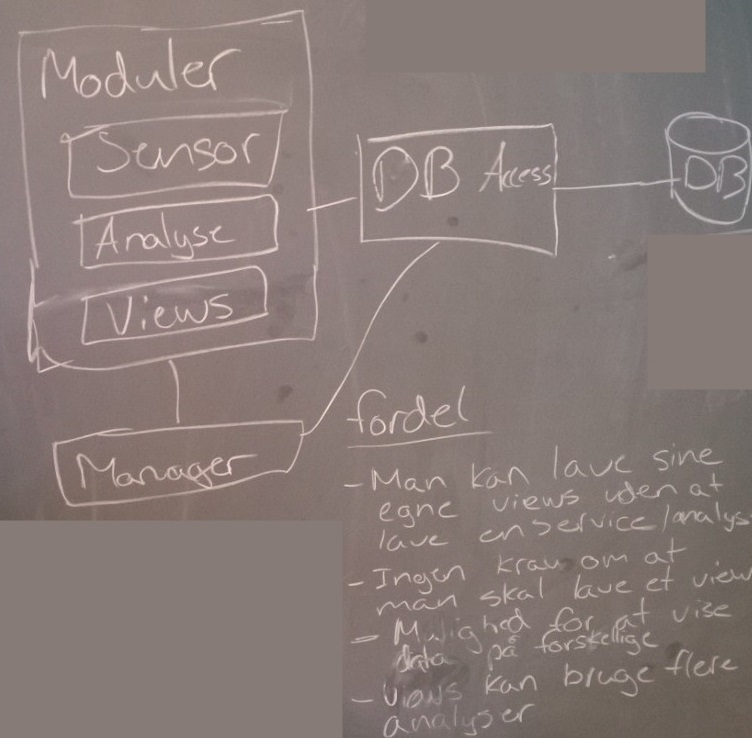
\includegraphics[width=\textwidth]{architecture_draft}
	\caption{Første udkast til arkitektur.}
  \label{arkitektur_udkast_1}
\end{figure}
Som nævnt herover er styrken ved denne arkitektur, den modulære opbygning af sensorer, analyser og visninger.
Disse lag er derfor alle indholdt i den overordnede komponent \textit{moduler}.
Derudover eksisterer et system, bestående af de resterende tre komponenter, der anvender de moduler der er installeret på den enkelte telefon.
Systemet er altså opbygget uden direkte kendskab til de enkelte moduler, hvilket igen tillader udviklingen af moduler sideløbende med det overordnede system.

Herunder gives en kort beskrivelse af hver af de fire komponenter.
Komponenterne beskrives i rækkefølge af deres indbyrdes afhængighed, således at forståelsen af hver komponent kun afhænger af det læste.

\subsection*{DB}
Denne komponent administrerer data for systemets forskellige moduler.
Data opbevares i en række tabeller i et relationelt database system.
Hvert modul har mulighed for at definere egne tabeller, der alle gemmes i \textit{DB} komponenten.

Til dette projekt er valgt en sqlite database da denne er standard i android.

\subsection*{DB Access}
Denne komponent styrer adgangen til \textit{DB} komponenten så det sker på en ensrettet måde.
\textit{DB Access} holder derudover styr på hvilke komponenter og lag der må skrive og læse fra de enkelte tabeller.

Systemet anvender udelukkende en database placeret på selve mobiltelefonen og er dermed begrænset af de muligheder der er for lagring på den enkelte enhed.
I en fremtidig udvidelse af systemet kunne \textit{DB Access} laget tilgå et ekstern lager hvor dele af det administrerede data kan gemmes.
Denne abstraktion forventes at kunne påføres \textit{DB Access} uden at kræve ændringer i de resterende komponenter.

Muligheden for en sådan udvidelse af systemet er ikke undersøgt og der kan derfor naturligt være komplikationer herved, ligesom udvidelsen ikke med sikkerhed kan laves uden påvirkning af de resterende komponenter.

\subsection*{Moduler}
Denne komponent består af tre konceptuelle lag: \textit{sensor}, \textit{analyse} og \textit{views}.
Alle moduler indeholder en modulbeskrivelse som beskrevet i \cref{modul_definition}. 
Alle moduler kan skrive til deres egne tabeller i databasen, samt læse fra alle andre modulers tabeller.

\stefan{skal der være eksempler på sensorer, moduler, etc?}
\mikkel{jeg har tilføjet et eksempel på sammenhængende moduler i den introducerende tekst. skal vi have yderligere?}
\paragraph{Sensor} \textit{Sensor}laget indeholder alle de moduler der logger data fra sensorer eller logger data fra applikationer.

\paragraph{Analyse}
\textit{Analyse}laget indeholder alle moduler der bruger et antal \textit{sensor}moduler og analyserer det data for derefter at gemme det i en databasetabel.

\paragraph{Views}
\textit{Views}laget indeholder alle moduler der gør det muligt at visualisere de analyserede data.
Den angiver hvilke og hvor mange datatyper den kan vise.

\subsection*{Manager}
Denne komponent står for at holde styr på hvilke moduler der er installeret og opretter tabeller i databasen for dem.
\textit{Manageren} indeholder også et GUI så brugeren kan tilføje og fjerne moduler.
\textit{Manageren} har også logikken for hvilke \textit{analyse} moduler der kan vises i hvilke \textit{views}.
Desuden indeholder \textit{manageren} også et JSON skema for hver modul-type i \textit{moduler} komponenten.
\stefan{et eller flere skemaer? Muligvis har views anderledes skema, men analyse og sensorer har det samme}

\section{Komponenter}
For at lave en naturlig opdeling af kode samt ansvar er koden blevet delt op i forskellige komponenter her er der tale om manageren og data laget.
\subsection{Manager}
Manageren er den eneste komponent brugeren interagerer med.
Det er igennem manageren at brugeren vælger hvilke moduler der skal køre.
Det er også den der sørger for at de rigtige moduler kører på de rigtige tidspunkter.
Dette gøres ved hjælp af \texttt{TaskRunner}.
Derudover er det også manageren der sørger for at skaffe moduldefinitionen fra alle de installerede moduler.
Ydermere, giver manageren et overblik over de visualiseringsmoduler der er installeret samt have en måde at vise visualiseringsmodulerne på.
\subsubsection{Kørsel af Moduler}
Der er overordnet to måder hvorpå moduler køres; enten styrer de selv deres kørsel (kontinuerte kørende moduler) ellers administreres de af managerens \texttt{TaskRunner}, som er en \texttt{Service} der startes når mobilen tændes.
Både sensor- og analyse-moduler kan køre på disse to forskellige måder.

\subparagraph{Kontinuerligt kørende moduler}
Til moduler der skal køres kontinuert, startes deres \texttt{Service} så snart modulet aktiveres i indstillinger, hvorefter det selv administrerer hvornår og hvor ofte det udfører sin opgave.
Dette er for moduler der skal samle kontinuert data ind, som fx et modul der bruger accelerometer.

\subparagraph{TaskRunner}
Derudover er der også moduler, som kun skal køres på faste intervaller eller bestemte tidspunkter.
Her er der ikke behov for at det enkelte modul har en kontinuert kørende \texttt{Service}, idet Manageren starter modulets opgave på det korrekte tidspunkt.
På denne måde spares der ressourcer, da modulet kun aktiveres i den tid hvor det skal udføre sin opgave. 

Når \texttt{TaskRunner}en startes, danner den en liste over de moduler der skal køres med interval eller på fast tidspunkt.
Derefter laver den en prioriteret kø, sorteret efter næste kørsels-tidspunkt.
\texttt{TaskRunner} tråden venter så, indtil næste opgave skal udføres.
Efter opgaven er udført udregnes næste kørsels-tidspunkt for den netop kørte opgave, hvorefter prioritets-køen sorteres.
Så venter tråden igen, indtil næste kørsels-tidspunkt, og dette fortsætter så længe der er aktive moduler, som skal køres på denne måde.

\subsubsection{Indstillinger}\label{sec:settings}
En af komponenter der skulle laves var en side der kan aktivere eller deaktivere moduler, det vil sige en indstillings side. Dette afsnit beskriver dette.

%guidelines
For at få en velkendt og standardiseret brugergrænseflade fulgtes android design guidelines.
Disse guidelines angiver hvornår man skal bruger diverse knapper, actionbars, settings etc.
\cite{androiddesign}

%Prototypes
Ved at følge disse guidelines blev en række prototyper for indstillinger lavet.
Disse byggede på samme princip om at udarbejde en indstillingsmenu.
Der var diskussion om hvordan disse skulle være, men over flere iterationer valgtes der at gå fra en ``wizard'' tilgang til en regulær settings menu,
Billeder af diverse prototyper kan ses i \cref{fig:prototype-manager}

\begin{figure}[H]
	\centering
	\begin{subfigure}[b]{0.45\textwidth}
			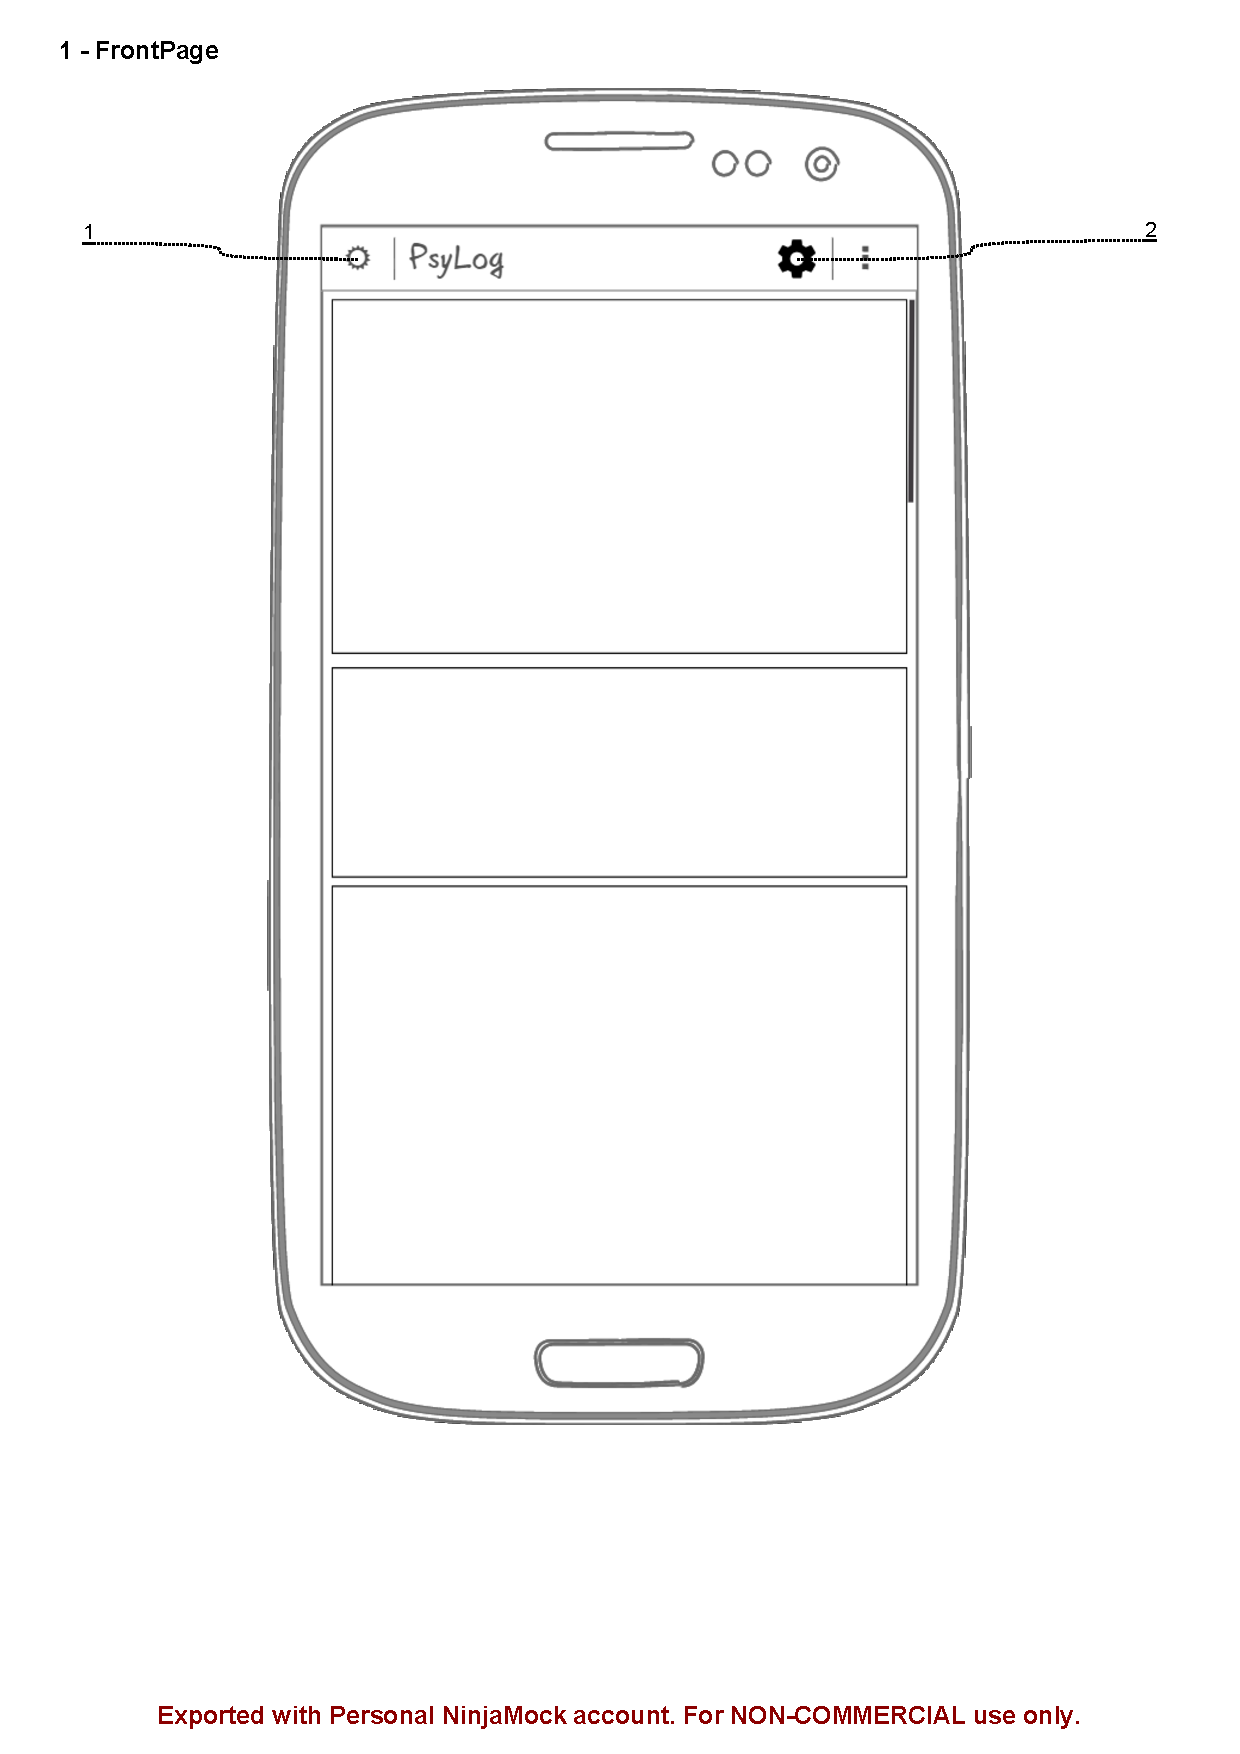
\includegraphics[scale=0.3, page=1, trim = 1cm 5.5cm 1cm 0cm, clip]{prototype.pdf}
			\caption{Forside}
	\end{subfigure}
	\begin{subfigure}[b]{0.45\textwidth}
			\includegraphics[scale=0.3, page=2, trim = 1cm 5.5cm 1cm 0cm, clip]{prototype.pdf}
			\caption{Indstillinger}
	\end{subfigure}
	\caption{Prototype af Manager}
	\label{fig:prototype-manager}
\end{figure}


%Actionbar
Ud fra prototypen kan en actionbar blandt andet ses, tanken er at følge et standard design hvor man har en actionbar i toppen.
Denne muliggør navigation til indstillinger, men også at gå tilbage til hovedmenuen, nuværende er der dog problemer med at den ikke vises under settings\als{Skal have lavet mere arbejde med den}

%Indstillinger, checkbox
Til at angive om et givent modul skal være aktiveret eller ej bruges checkboxes.
Dette skyldes at det er et simpelt ja/nej valg. 
Tanken er så at de moduler man har valgt er dem der kører på telefonen.

%indstillinger, dependencies og events
For at scanne mobilen for de moduler der er installeret bruges JSONParser der tager vare af dette. \als{referer til JSONParser}
Dette giver udslag i en række moduler der har afhængigheder af andre moduler og skal takles.
JSONParseren giver som resultat en liste af moduler. Disse scannes så igennem for at finde deres afhængigheder.
Disse afhængigheder bruges så til at konstruere events (OnChange) til at fortælle de moduler der skal have besked når et givent modul aktiveres/deaktiveres.
Ved at lave en sådan række er der implicit konstrueret en dependency graph.
Og som resultat af dette kan man forestille sig et hierarki hvor et modul på det lavest liggende niveau medfører en kæde af deaktiveringer af moduler der eksplicit og implicit afhænger af dette modul.
\stefan{så vidt jeg ved sker dette ikke længere på samme måde, Winde (eller en der vil sætte sig ind i koden) bør nok revidere dette afsnit}

%indstillinger, onPause start og stop sensorer
Efter afhængighederne er enkodet i programmet mangler der at takle hvordan sensorer skal startes og stoppes fra indstillingsmenuen.
Til at takle dette bruger vi den allerede udviklede ServiceHelper\als{referer til denne}.
Der vælges så at starte og stoppe de fornødne sensorer i onPause, da det typisk er når man forlader en indstillingsmenu at man gerne vil have at indstillingerne træder i kraft, og sikrer også at man ikke skal klikke på ekstra knapper for at indstillingerne træder i kraft.
\subsubsection{JSON-Parser}\label{subsub:JSONparser}\mikkel{Find på bedre navn}
JSON-parserens job er at finde JSON filen for hvert eneste modul installeret på smartphonen, hvorefter dette parses over i en klasse, og derefter autogeneres klasser ud fra JSON filen.
Måden dette er gjort på er ved brug af `jsonschema2pojo' \citep{jsonpojo}, der gør det muligt at få genereret klasserne som passer til JSON skemaerne, men også at få parset JSON filerne over i en klasse. 
\subsection{Data Lag}
Dette afsnit detaljerer data laget i det overordnede system. 

\subsubsection{Database}
Det er nødvendigt at lagre data fra moduler så andre moduler kan bruge dataene.
I Android er det standard at data kun er tilrådighed til den specifikke applikation der har lagret det.
Applikationen gøre sin data tilrådighed for andre via en \texttt{ContentProvider}.

\subsubsection{Samlet i manager VS i hver app}
Der er undersøgt to muligheder for gøre data tilgængelig.
Man kan samle data fra alle moduler i manageren da denne står for den overordnede kontrol af systemet. 
Manageren kan da definere et interface til databasen, som så moduler bruger til at læse eller skrive data. 
Den anden mulighed er at hvert modul direkte lagrer data i deres egen database, og så gør den tilgængelig for de moduler der vil bruge den.
Vi vælger at samle al data i manageren, da det stærkt simplificerer adgang til databasen, da hvis individuelle databaser var blevet brugt til hvert modul vil dette påkræve opsætning af databaser i hvert eneste modul.
Derudover simplificere det også backup og udvælgelse af data hvis det ligger samlet.

\subsubsection{Database Helper}
For at lave databasen i manageren skal der oprettes rettigheder til at kunne læse/skrive til databasen samt lave nye database tabeller.

\subsubsection{ContentProvider}
En content provider er en android konstruktion der giver adgang til data for andre applikationer.
ContentProvider er en abstrakt klasse, hvor subklasser skal overskrive 5 metoder:  getType, query, insert, delete og update. \cite{contentprovider}

Insert gør det muligt at skrive til databasen, query læser fra databasen, delete sletter og update opdaterer eksisterende data.

getType er en metode der benyttes til at angive MIME typen af data ContentProvideren giver adgang til.

I den nuværende implementation er det valgt kun at implementere insert og query da det er de eneste relevante funktioner i forhold til det behov vi har på nuværende tidspunkt, hvor vi kun er interesserede i at læse fra og skrive til databasen.

Delete kan blive relevant til brug ved oprydning af for gammel data. Da vi fokuserer på at analysere på mønstre i dataene kunne man eksempelvis slette sensor data der er ældre end 2 måneder. 
Alder på data til sletning kan afhænge af datatype, eksempelvis kunne man forestille sig at bevægelsesdata kan slettes efter kort tid mens sociale interaktionsdata skal leve længere.
\section{Modul-Definition}\label{modul_definition}
%Måde at lave eksterne modul-applikationer uden at ændre hoved-applikation.
%Definere output (tabeller/kolonner), samt input (afhængigheder)
%Evt. konfigurationsmuligheder for moduler afhængige af det
%Fleksibel måde at modtage data fra andre moduler, uden at skulle opdatere applikation(erne). Dvs. ikke design-mønstre: observer, mediator, men gennem content provider.
% modularisering i Android; multiple applikationer under samme package

For at opfylde kravet om fleksibilitet der er stillet til systemet, har vi udtænkt en modulbaseret arkitektur der gør det let at tilføje moduler til pakken.
Det skal være muligt at tilføje eksterne moduler, uden at have behov for at lave ændringer i hoved-applikationen.
Dette kan gøre sig gældende når der kommer nye sensorer på markedet, eller hvis der skal laves nye former for visualiseringer til det allerede indsamlede data.
\subsubsection{Forslag til modulariseing}
\paragraph{Komplet Pakke}
En traditionel applikation samler al funktionalitet i en pakke.
Hvis man udvikler på dele af applikationen vil en opdatering skulle ske af hele appen på samme tid.
Desuden bliver det sværere for eksterne udviklere at bidrage til applikationen, da opdateringer skal ske igennem udviklerne af hovedapplikationen.

\paragraph{Import af Kode}
En anden mulighed er at inkludere et scripting sprog med applikationen og gøre det muligt at udvikle script der kan agere modul.
Denne løsning kræver et meget kraftigt scripting sprog hvis alle Androids muligheder skal stilles til rådighed.
Hvis scripts på den anden side skal skrives direkte i java vil der være nogle sikkerhedshensyn som vil gøre det svært at kontrollere hvad moduler kan og ikke kan.
For eksempel vil det være vanskeligt at kontrollere hvilke database tabeller der er adgang til.
Sikkerhedsproblemet er stort, men kunne sikkert løses med nok tid og ressourcer.

\paragraph{Selvstændig Applikation}
Den tredje mulighed er at pakke hvert modul i en selvstændig APK \footnote{Androids pakkeformat}.
Denne APK skal indeholde en beskrivelsesfil som læses i hoved-applikationen og indeholder information om modulet.
Denne metode sørger for at hoved applikationen kan kontrollere hvad moduler har adgang til. 

Ulemper ved denne løsning er at den er knap så lightweight, idét at det kræver at en stor mængde af applikationer skal installeres.
Derudover er kommunikation mellem applikationer vanskeligere end internt i en applikation, men ses som acceptabelt.
Desuden kan det være træls at skulle installere en større mængde af applikationer for at have den fornødne funktionalitet.
Som løsning derpå kunne man med videre arbejde have et indbygget applikation marked i manageren, og er værd at udforske med mere tid.

Det er en løsning der har mange fordele i forhold til modularisering og svagheder der kan tolereres, hvorfor denne løsning er valgt. 

Det følgende vil forklare detaljerne i implementationen af moduler ved hjælp af selvstændige applikationer.

\subsubsection{Beskrivelsesfilen}

Til dette er der valgt at bruge JavaScript Object Notation (JSON) samt JSON Skema \citep{jsonpojo}.
Eksemplerne der bruges herefter vil derfor være i henholdsvis JSON eller JSON Skema.

\subsubsection{Typer af Moduler}
Der findes som sagt i \cref{sec:arkitektur}, tre typer moduler: \textit{sensor}, \textit{analyse} og \textit{visualisering}.
Som sagt er sensor moduler, moduler som indsamler data fra telefonens forskellige sensorer og applikationer.
Endvidere er analyse moduler, moduler som bruger data fra enten sensor eller andre analyse moduler til at bearbejde data med den hensigt at opnå en opsummering af data som kan videre bruges af systemet til enten visualisering eller videre bearbejdning.
Visualiseringsmodulerne bruges til visualisering af den rå sensor-data eller den behandlede analyse-data.

\subsubsection{Moduldefinition}
Som minimum har et modul et navn og en version, så andre moduler kan referere dem.

Sensor- og analyse-moduler skal gøre data tilgængeligt for andre analyse- og visualiserings-moduler.
For at specificere hvordan data skal gemmes, samt hvad der er tilgængeligt for andre, skal dette defineres for hvert modul af førstnævnte typer.
For hvert modul skal der defineres en eller flere tabeller som modulet kan gemme data i.
For hver tabel defineres en eller flere kolonner med et beskrivende navn, datatype og evt. en måleenhed.

\subsubsection{Data Typer}
De tilgængelige data typer tilgængelig for tabel-kolonner, er begrænset til de tilgængelige SQLite datatyper.
Der er 5 typer: \textit{NULL}, \textit{INTEGER}, \textit{REAL}, \textit{TEXT} og \textit{BLOB}.

\subsubsection{Afhængigheder}
Et analyse- eller visualiserings-modul kan være afhængigt af andre sensor- eller visualiserings-moduler.
Et analysemodul kan aggregere data fra andre analysemoduler mens et visualiseringsmodul er afhængig af det modul det skal vise data fra.
Derfor skal det defineres for hvert modul hvilke andre moduler det er afhængigt af.
Der findes to grader af afhængigheder i systemet: hard- eller soft-dependency.
En hard-dependency er ét andet modul som det pågældende modul ikke kan fungere uden.
En soft-dependency er en liste af andre moduler, hvor mindst ét af de listede moduler skal være til stede på enheden.
Dette er nyttigt hvis et modul skal bruge eksempelvis accelerometer data, men det er ikke vigtigt om det kommer fra en telefon eller fra en wearable.

\subsubsection{JSON og JSON Schema}
For at have en modul-beskrivelse der er læselig for både mennesker og maskiner, er JSON valgt.
JSON gør det muligt for ikke-tekniske personer at læse, skrive og forstå definitionen af et modul.
For at sikre validiteten af eksternt leverede modul-beskrivelser, udarbejdes der et JSON Skema, som JSON-dokumenter kan holdes op imod og derved verificeres.
Det anvendte JSON Skema kan findes i \cref{app:json_schema}.

\paragraph{Eksempel} på en modul-beskrivelse.
Meta-data er præfikset med \_ (underscore).
\begin{lstlisting}
{
  "name": "accelerometer",
  "_version": 1.0,
  "tables": [
    { "name": "accelerations",
      "columns": [
        { "name": "accX",
          "dataType": "REAL",
          "_unit": "g" },
        { "name": "accY",
          "dataType": "REAL",
          "_unit": "g" },
        { "name": "accZ",
          "dataType": "REAL",
          "_unit": "g" }
      ]}]}
\end{lstlisting}

\subsubsection{Implementering}
Som nævnt i \cref{sec:valg_af_android}, implementeres der til Android telefoner.
Dette sætter nogle begrænsninger ift. valg af løsninger.

\subsubsection{JSON kontra XML}
XML ville være det naturlige valg for Android applikationer, da en del af applikations udvikling foregår i XML fordi man ofte bruger det til at definere layouts og definering af statiske ressourcer. 
Dog blev JSON valgt over XML, da vi gerne ville have automatisk generering af en parser ud fra skemaet.
En automatisk genereret parser vil lette arbejdet med et skema der i udviklingsperioden ændres ofte.
Denne automatiske generering viste sig ikke at være ligetil på grund af kompatibilitetsproblemer på Android, mens det var enkelt at udføre i JSON.

\subsubsection{Moduler som Applikationer}
For at det skal være muligt at installere moduler uden at opdatere hoved-applikationen, skal der installeres applikationer via Google Play Store.
Alle modul-applikationer, samt hoved-applikationen, deler \textit{package}-navn.
Hver modul-applikation har sin JSON beskrivelse som en eksternt tilgængelig \textit{ressource}, som hoved-applikationen eller andre moduler har adgang til.
Kommunikation mellem applikationer foregår med \textit{services}, \textit{intents} eller \textit{content provider}.

\subsubsection{Håndtering i Manager}
Håndteringen af moduler sker i manageren, beskrevet i \cref{subsec:arkitektur-Manager}.
Når der tilføjes eller opdateres et modul detekterer manageren dette ved at finde alle applikationer der er installeret under pakken ``dk.aau.cs.psylog''.
Manageren læser alle moduldefinitioner efter at have valideret dem op imod JSON skemaet.
Alle moduler der har opdateret versionsnummer eller er helt nye vil blive håndteret ved at manageren læser tabelinformation ind fra moduldefinitionen og opretter eller ændrer de pågældende tabeller.

Når modulernes tabeller er blevet oprettet bygges en graf over afhængigheder, som bruges til at vise brugeren hvilke moduler der kan aktiveres.
Denne proces er yderligere beskrevet i \cref{sec:settings}

\subsubsection{Visualiserings Modul}\label{sec:visningsmodul}
Som udgangspunkt er \textit{visualiseringer} forskellige visualiseringer af analyse modulernes output.

De eneste restriktioner der stilles for data der kan læses fra et analyse moduler er de formater der kan gemmes i databasen.
Det betyder at det mulige output fra et analyse model er meget fleksibelt, hvilket kræver en tilsvarende fleksibilitet i visualiseringsmodulerne.

En simpel løsning vil være at der for hvert analysemodul skal defineres et visualiserings modul.
Herved sikres det at alle analysemoduler har en visualisering der præcist repræsenterer genererede data.
Det er dog nemt at finde problemstillingerne i denne løsningsmodel, da det giver meget lav genanvendelse af eksisterende moduler.
Eksempelvis kan man nemt forestille sig forskellige datasæt der kan repræsenteres ved hjælp af en to-dimensional graf.
En løsning der ville kræve en ny implementation af en sådan visualisering for hver analyse modul er ikke fleksibel nok.

Alternativt kan visualiseringer beskrive en liste over de analyser de kan anvendes på.
På den måde kan visualiseringer anvendes på mere end et analyse modul.
Omend dette løser problemet til en vis grad vil problemet stadig eksistere når der tilføjes nye analyse moduler.
Her vil visualiseringerne enten ikke have kendskab til de nye moduler eller de vil skulle opdateres løbende.
Altså er fleksibiliteten af denne løsning heller ikke god nok.
Man kan naturligvis også lade alle analyse moduler beskrive en liste over visualiserings moduler.
Men denne opbygning vil give samme problemstilling som beskrevet herover.

En mere fleksibel metode til håndtering knytningen mellem visualiseringer og analyser er at deducere ud fra analysens tabel/kolonne signatur, hvilke slags data der kan aflæses.
På denne måde kan der laves visualiseringer der repræsenterer bestemte signaturer, og der opstår en implicit binding mellem visualiseringer og analyser for de hvor de to beskrivelser stemmer overens.

I mange tilfælde vil denne implicitte binding være nok, dog kan det forestilles at analyserne vil være forskellige og til tider komplekse, hvilket kan gøre det nødvendigt at nærmere specificere hvordan den tilgængelige data kan vises.
Der er også den mulighed at analysemoduler kunne have ekstra database tabeller, der ikke skal vises, som så kunne virke forstyrrende for den implicite binding.
Her kunne der tilføjes noget meta-data på analysens tabeller/kolonner, der beskriver den på sådan en måde, at det ville kunne bruges til visualiseringer der ikke nødvendigvis implicit kunne knyttes til det.
Det kunne også være muligt at tilføje information om kriterier for visualiseringer i analysemodulers JSON filer, og så overlade det til Manager komponenten at matche et analysemoduls kriterier med de kriterier visningsmoduler opfylder.

\subsubsection{Eksempel}
Her bruges light, som er en simpel sensor og analyse, der fra sensoren indhentes løbende lys-niveau (i lux).
Analysen tager den senest indsamlet data og giver et gennemsnit.
Det antages at alle tabeller har en tids-kolonne, der beskriver enten hvornår data blev indsat i databasen, eller i nogle tilfælde af analyser overføres tiden fra sensor-data.

\begin{lstlisting}
{
  "name": "lightAvg",
  "_version": 1.0,
  "tables": [
    {
      "name": "lightAvg",
      "columns":[
        { "name": "lightAvg", "dataType": "REAL", "_unit": "lux" }
      ]
    }
  ],
  "dependencies": [
    [{ "name": "light" }]
  ]
}
\end{lstlisting}

Et eksempel på et visualiserings-modul som passer på denne type analyse kunne være en simpel 2D graf, som viser den gennemsnitlige belysning over tid.

\begin{lstlisting}
{
  "name": "2dgraph",
  "_version": 1.0,
  "_type": "view",
  "view": {
    "layout": "2dgraph.xml",
    "data": [
      { "name": "x", "dataTypes": ["INTEGER"], "fromTimestamp": true },
      { "name": "y", "dataTypes": ["INTEGER", "REAL"] }
    ]
  }
}
\end{lstlisting}
 
Denne visualisering beskriver en 2D graf, som bruger layoutet i \texttt{2dgraph.xml}.
På x-aksen vises tiden (der står INTEGER fordi SQLite ikke har datorepræsentation ud over unix-time).
Her bruges det tidsstempel som forventes på alle tabeller.
Til y-aksen kan bruges alle analyser, som blot har en enkelt kolonne af heltal eller decimal-tal værdi.

\subsubsection{Administrering af Visualiseringer}
Ligesom sensorer og analyser, skal visualiseringer også administreres af brugeren.

For at holde det så simpelt som muligt, kunne man, ligesom ved sensorer/analyser, have to niveauer af administration.
Som udgangspunkt vil alle installerede visualiseringer automatisk knytte sig til de aktiverede analyser.
Derudover vil man i de avancerede indstillinger kunne aktivere/deaktivere visualiseringer for de enkelte analyser.

På denne måde vil der automatisk blive genereret en liste af visualisering/analyse kombinationer, men med mulighed for at slå nogle af kombinationerne fra.
Det vurderes at muligheden for at slå visualiseringer fra skal være under avancerede indstillinger, da ikke teknisk erfarne brugere sagtens kunne forvirres af alle de potentielle visualisering/analyse kombinationer de ville præsenteret for.
Grunden til at det stadig er med som en mulig customization er, at der er stor fokus på at brugerne skal have mulighed for at styre hvad programmet skal gøre. 



\chapter{Refleksion}
I udviklingsforløbet af platformen, var der forskellige beslutninger, som blev taget i henhold til hvad der skulle implementeres, samt hvad der kunne udvikles videre på og generelle overvejelser om platformen.
At reflektere over disse beslutninger og overvejelser skaber overblik og forståelse af forløbet, og er beskrevet herefter.

%\section{Valg af data kilder}
%Hvilke data kilder man bruger i for eksempelvis et analyse modul kan være vigtige, idet hvis man for eksempel har data fra et smartwatch og fra en accelerometer på smartphonen og en af disse viser ingen bevægelse ville det være en god idé at hvis modulet selv kunne evaluere hvilke kilde den skal tage data fra. 
%Men dette blev aldrig lavet, idet det ikke var tænkt særlig vigtigt og at ressourcerne var begrænsede og skulle bruges på andre opgaver i stedet for.

\section{Kontekst}
Konteksten for brugen af applikationen er ikke blevet arbejdet med.
Man kunne forstille sig at der kunne være indbyggede moduler til at registrere hvilket kontekst smartphonen befinder sig i.
Dette kunne være at finde ud af om smartphonen befinder sig på en person eller om den er i en jakkelommer, på et natbord eller lignende.
Hvis det er muligt at identificere konteksten, kan det være yderst brugbar information for analysemoduler, til at hjælpe dem med at afgøre hvordan forskellige former for data skal behandles.
Her kunne man for eksempel forestille sig at lyd var yderst relevant hvis enheden var på en person, men irrelevant hvis den lå i en jakkelomme.
Der er også den mulighed at platformen ud fra konteksten vælger hvilke datakilder, der stadig er relevante at se på, men en sådan måde at beslutte på vil reducere platformens modularitet, så det vil være bedre at overlade det til det enkelte modul at beslutte hvad der er relevant for den givne kontekst.

Dog vides det ikke om en sådan klassificering kan opnå den fornødne præcision, men undersøgelse af det vil bestemt være værd at overveje.

\section{Brugerinteraktion}
En række refleksioner går på brugerinteraktion.
Dette inkluderer refleksion af visualiseringer, interaktive moduler, notifikationer og huskekort, hvilket er beskrevet herunder.

\subsection{Visualiseringer}
Data indsamlet og analyseret af forskellige moduler, skulle originalt kunne visualiseres, med det formål at give brugere af platformen et overblik over deres sindstilstand.
I \cref{modul_definition}, blev der diskuteret hvordan håndteringen af visualiserings-modulerne skal foretages.
Dette er et emne, der bør udforskes ved videre arbejde, men er ikke foretaget på nuværende tidspunkt, da det blev dømt for tidskrævende.
Ved videre arbejde bør datavisualiserings-teknikker og -teori undersøges nærmere.

\subsubsection{Hvordan skal brugeren vælge visualiserings moduler?}
Udover diskussion om hvilke krav der skal være til visualiserings-moduler, beskrevet i \cref{modul_definition}, skal man også overveje hvordan brugere skal vælge hvilke visualiserings-moduler de gerne vil kunne se, og hvordan de skal vises i manageren.

En mulighed er at have en administrationsside til visualiseringer, der minder om indstillingssiden til valg af dataindsamlings- og analysemoduler.
Eksempelvis kan man forestille sig en kobling mellem disse moduler og visualiseringerne, sådan at for hvert modul kan man angive hvilke visualiseringer man vil benytte.
Koblingen ville her gå på visualiseringer, der passer til de enkelte datasæt som modulerne tilbyder.

En anden mulighed er at visualiserings-modulerne, der er installeret, er dem der bliver vist i manageren, og specificerer selv hvilke moduler de virker til.
Dette er en mere enkel løsning at implementere, til gengæld tilbyder den knap så stor fleksibilitet i forhold til udviklingen af nye analysemoduler, da man så er nødsaget til at skulle opdatere specifikationen for de pågældende visualiserings-moduler.

\subsubsection{Hvordan skal visualiseringer vises i manageren?}
En anden diskussion går på hvorledes visualiseringerne skal vises i manageren.
En enkel måde at gøre dette på er som en liste, der bliver præsenteret på forsiden af manageren.
Der vil med denne løsning være mulighed for at ændre rækkefølgen af modulerne ved at trække visualiseringerne til en anden position i listen.
En ulempe ved denne løsning er at den ikke tilbyder kategorisering af visualiseringer.

En inddeling af visualiseringerne i forskellige kategorier ved hjælp af faner er et alternativ, der kan benyttes.
Dette sikrer at hvis man har mange visualiseringer bliver det nemmere at abstrahere over disse, da man kan nøjes med at se på en kategori ad gangen, eksempelvis søvn eller social aktivitet.

\subsubsection{Hvordan skal visualiseringer gøres forståelige?}
Endvidere er der en overvejelse, som går på at udvikle visualiseringer, der er forståelige og gennemskuelige for målgruppen, men dette betragtes som et ansvar for den enkelte visualiserings-udvikler og er dermed ikke noget platformen bør takle.
Platformen benyttes af udvikleren, men hvordan de enkelte visualiseringer skal se ud er op til den enkelte udvikler.

De præsenterede muligheder er ikke fastlagte, og opfordres til at blive diskuteret yderligere ved videre arbejde, så den mest hensigtsmæssige løsning opnås.

\subsection{Interaktive moduler}
En idé, som ikke blev undersøgt var at udvikle interaktive moduler.
Eksempelvis kunne patienter blive sat til at løse matematiske problemer for at teste deres kognitive evner eller spille `balance the ball' for at teste deres reaktionsevne.
Dette kunne være en god idé, da man ved affektive lidelser nogle gange ser den slags symptomer, for eksempel ved depression kan man tit opleve at man har svært ved at huske detaljer, tage beslutninger eller koncentrere sig og hvis spil kunne laves for at teste disse kunne man få et indblik i hvordan patienterne har det. 
En yderlig grund til at undersøge og implementere dette er, at det vil gøre systemet mere interessant for brugerne og give dem en grund til at bruge det hver dag. 
Et sådant modul ville klassificeres som en mellemting mellem et visualiserings modul og et sensor modul.
Visualisering da modulet skal vise noget til brugeren og sensor da den giver data, der kan bruges af analysemoduler til at få et indblik i folks tilstand.

\subsection{Notifikationer}
Noget, som også blev diskuteret tidligere i projektforløbet var at give notifikationer til brugeren, herunder det, som tidligere er benævnt som interventioner.
Dette blev dog tilsidesat, da det blev vurderet at der var for mange faldgruber i.f.t. at forstyrre en evt. patient med psykiske problemer.
Dog erfarede vi senere, i forbindelse med styregruppemødet, at patienterne er meget interesseret i at få at vide så tidligt som muligt om de er under forværring i deres tilstand.

Der kunne eksempelvis gives to slags informationer; interventionen, som direkte siger at der foregår en forværring eller at der har været en drastisk stigning/fald i.f.t. sensor/analyse.
Den anden slags information kan være noget opsummerende og mere neutralt, så der ikke på samme måde skal evalueres om hvorvidt der er ved at ske en forværring, derimod blot præsentere noget af det seneste data fra en sensor/analyse.
Det andet eksempel på en notifikation kunne få brugeren til at reflektere over sin situation, hvis der for eksempel kunne ses et tydeligt fald i søvnkvalitet eller antal sociale interaktioner, men uden direkte at sige noget om en evt. forværring.

\subsubsection{Huskekort}
I interviewet med psykolog Janne Vedel Rasmussen blev huskekort nævnt, se \cref{sec:moede-med-psykolog}.
Disse dækker over nogle fysiske huskekort som patienten har på sig, hvorpå der står en form for instruktioner, der kan assistere i svære situationer; hvor dette eksempelvis kan være at ringe til en ven før en svær beslutning skal træffes eller at droppe den nuværende opgave og i stedet foretage en lystbetonet aktivitet.

Disse kan på samme måde som benævnt ovenover også implementeres som notifikationer.
På denne måde kan der foreslås en lystbetonet aktivitet hvis analyser antyder en stressende dag.
Dette er især interessant ved fysisk sensor/analyse hvor stress antageligvis kan opdages i øjeblikket og et passende huskekort kan præsenteres.

Disse huskekort skal dog nødvendigvis udarbejdes sammen med patientens behandler, da antal, type og indhold af huskekort varierer.

\section{Platform}
Andre refleksioner går på platformen.
Disse refleksioner omhandler hvordan man kan mindske plads- og strøm-forbrug, alternativer til moduldefinitions-deling, samt hvordan en højere granularitet kan opnås hvad angår databaserettigheder, og er beskrevet herunder.
Ydermere reflekteres der også om platformens styrker og svagheder.

\subsection{Dataindsamling}
Som nævnt i \cref{eksperimenter}, blev der udført eksperimenter for at få en idé over hvor meget plads der kræves for at kunne benytte platformen.
Ydermere siger den at mængden af data der indsamles kan blive reduceret.
Der nævnes tre forskellige måder dette kan gøres på, hvilket er ved brug af skyen, komprimering af data eller ved at ændre på opdateringshastigheden for de forskellige sensorer.
I den sammenhæng er det vigtigt at vægte fordele og ulemper for metoderne, samt om det er muligt at kombinere de forskellige metoder.
En kombinering man kunne forstille sig er at lagre gammelt data i skyen, hvorimod ny data lagres lokalt, men hvor al data komprimeres.
Hvordan dette skal implementeres er et åbent spørgsmål, men bør udforskes videre.
Som udgangspunkt har vi lavet et interface, som modulerne kan benytte, i form af DBAccess, så disse ændringer ville være backend ændringer og dermed ville de ikke komme til at påvirke de enkelte moduler.


En anden tankegang til at reducere plads er ved at ændre arkitekturen så man kan kommunikere modul til modul uden nødvendigvis at lagre i en database.
En fordel ved dette kan være at moduler kan sende deres opsamlede data til andre moduler, så man kan undgå helt at gemme data i databasen for visse mellemleds-moduler.
På den måde vil man kunne spare en masse plads, men det vil komme på bekostning af at det ikke længere er muligt at rekonstruere en analyse. En måde dette kunne implementeres på, uden at gå på kompromis med modulariteten, er at benytte sig af et observer designmønster som beskrevet i \cref{subsec:DBACCESS}.
Dog er det en stor ændring i forhold til den nuværende arkitektur, men er et alternativ man med fordel kunne benytte sig af til at gøre datadeling mellem moduler mindre pladskrævende.

Når en eller flere af disse er implementeret, er det en god idé at gentage eksperimenterne for at verificere at løsningerne har den ønskede effekt, og på samme tid vil det være fordelagtigt at udvide eksperimenterne til at inkludere andre faktorer såsom batteri forbrug.

\subsection{Analyse i skyen}
For at aflaste smartphonen, er det allerede blevet forslået at bruge skyen til at opbevare data, men på samme tid kan analyser fordelagtigt også blive udført på skyen. 
Dette vil have den effekt at smartphonen ikke behøver gøre særlig meget udover at registrere sensor data.
Dette er også en idé, der bør undersøges videre, hvor man også skal have problematikker såsom sikkerhed og kommunikationstid i mente.

\subsection{Alternativ moduldefinitions-deling}
Med den nuværende implementering skal platformen hente ressourcefilerne for de enkelte moduler, for at læse deres moduldefinitioner.
Med denne løsning har andre applikationer dog også rettighed til at læse ressourcefilerne, hvilket normalt ikke er muligt med Android applikationer og det er på samme tid heller ikke den ønskede måde at dele filer på i Android.

Til at undgå denne metode af deling, bør der ved videre arbejde blive set på andre metoder til at dele filer.
En mulig metode var at bruge en fileprovider.
En file provider kan gøre det muligt at dele en bestemt fil og er den officielle måde at dele filer på i Android.
Vi nåede dog frem til at brugen af fileprovider havde en væsentlig ulempe.
Det var nødvendigt for platformen at vide hvilke fileproviders der skulle bruges, hvilket gør platformen væsentlig mindre modulær, da tilføjelse af et modul også vil kræve ændring i platformen.

Vi tager det forbehold at andre alternativer kan benyttes vi ikke har kendskab til, og hvis en sådan løsning findes bør denne benyttes da den nuværende løsning ikke er idéel, idet det ikke er sådan man skal dele filer mellem applikationer på Android.

\subsection{Databaserettigheder}\label{databaserettigheder}
Med den nuværende implementering af DBAccess har hvert modul adgang til alt data som ligger i databasen.
Dette er unødvendigt åbent og giver for bred adgang til de forskellige modulers data.
For at gøre løsningen mere sikker, bør der med videre arbejde implementeres en måde til at begrænse hvilke moduler, der har adgang til hvilket data.

En ønsket mulighed er at gøre det internt i platformen, idet man kan definere tilladelser i moduldefinitionen og baseret på disse give tilladelse til tabeller. 
Dette har ikke været muligt at implementere, da man fra DBAccess' vinkel ikke kan blive orienteret om hvilket modul benytter den, dette er en begrænsning fra Androids side.

En måde at løse dette problem på er ved en nøgleudveksling mellem manager og modul når et modul installeres, hvor hvert modul får en unik nøgle man sender med, så manageren kan kende forskel på moduler.

\subsection{Styrker og svagheder}
Platformen har forskellige styrker og svagheder, disse bliver dokumenteret herunder. 

Platformen er meget modulær, idet det er simpelt at tilføje nye moduler til den. % Styrke
Dette har dog den betydning at brugeren potentielt skal installere mange applikationer, hvilket selvfølgelig kan være forvirrende hvis de ikke ved hvad de skal bruge. %svaghed
Man kunne måske her forstille sig en fremtidig løsning hvor systemet anbefalede hvilke applikationer, der skulle hentes for at lave bestemte analyser, og måske endda at det var muligt at installere dem gennem platformen.

Platformen har det problem at størrelsen af data den gemmer kan give problemer og lige nu er der ikke blevet implementeret noget, som kan håndtere dette på en hensigtsmæssig måde. % Svaghed

Denne mængde data kan tage lang tid at bearbejde og analysere, hvorfor nogle moduler har måder, der gør det nemmere at håndtere meget data såsom at tage det lidt af gangen.
Idet platformen tillader dette er det en styrke. % Styrke

Platformen er meget åben, idet den deler adgang til databasen og ressourcefiler, hvilket gør det meget nemt for modulerne at få adgang til de data de skal bruge. 
Der kan dog gøres et argument for at det er for åbent, idet alt for meget data deles og ikke bare hvad modulerne skal bruge. 

\lasse{Hvis der er nogen som har nogle andre styrker og svagheder må de godt skrive dem her.}

\chapter{Konklusion}
Der kan konkluderes at en platform er blevet udviklet, der understøtter udviklingen af dataindsamlings- og analyse-moduler.
Et bevis derpå kan findes i \citet{misc:soevnrapp} og \citet{misc:surveyrapp}, hvor udviklingen af søvnestimeringsmoduler, aktivitetsmoduler, surveymoduler, opkald og sms/mms moduler er beskrevet.
Dette hænger fint i tråd med F-16 flyet som en metaforisk vision.
Tankegangen om at have en række moduler man kan hægte på platformen fungerer i praksis, men der er stadig en række problemstillingerne der bør arbejdes videre på som reflekteret ovenfor.

Derudover lød udfordringen på at udvikle en applikation til at overvåge adfærd for unipolare og bipolare patienter og gøre dem opmærksomme på adfærdsændringer.
Denne udfordring er ikke løst, men der er påbegyndt en løsning af problemet.
Fokus har gået på dataindsamlings- og analyse-aspektet af platformen, hvor det er blevet gjort muligt at udvikle moduler dertil, jævnfør tidligere nævnte udviklede moduler.
Vi kan konkludere at platformen har været tilstrækkelig modular og fleksibel til de udviklede moduler, men det er muligt at forbedringer kan foretages,
Det skulle dog være nemt at udvide platformen uden at skulle ændre på implementeringen af de enkelte moduler, da et facade designmønster er benyttet.
Platformen danner dermed grundlaget for videre arbejde, da med platformen udviklet bør der ved videre arbejde fokuseres på moduler til den efterfølgende registrering af ændring i adfærd og visualisering af analyser, baseret på analyseresulaterne af tidligere nævnte udviklede moduler.

Da fokus har været at facilitere dataindsamlings- og analyseaspektet af platformen mangler der at blive udforsket hvorledes visualiserings-moduler skal faciliteres.
Vi er klar over denne mangel, men det blev bedømt vigtigere at fokusere på at gøre det nemt at indsamle relevant data først, inden at der blev lagt fokus på hvordan man skulle visualisere data.

Med hensyn til kriterier er der også en række kriterier der kan konkluderes på.
Følgende kriterier der konkluderes på er de samme kriterier som blev opstillet i \cref{sec:process} og blev holdt i mente til udviklingen af platformen, beskrevet i \cref{arkitekturkrav}.
\begin{description}[style=nextline]
	\item[Modulær]
	Platformen er udviklet med primært fokus på at være modulær, og det kan konkluderes at den er det.
	Dette understøttes af den fælles datagrænseflade i form af DBAccess og moduldefinitionerne.  
	Det er muligt at specificere at man er afhængig af blot et modul af en mængde af disse.
	Eksempelvis er det muligt for et analyse modul at afhænge af minimum et accelerationsmodul, om dette så bliver fra en smartwatch datakilde eller det indbyggede accelerometer i mobilen afhænger af den enkelte patients installerede moduler.
	
	Som et eksisterende eksempel på at moduler nemt kan tilføjes og bruges af manageren er de nævnte udviklede moduler, beskrevet i \citet{misc:soevnrapp} og \citet{misc:surveyrapp}.
	Dette eksempel viser også hvorledes det er muligt at udvikle moduler, der afhænger af data fra andre moduler.
	
	\item[Fleksibilitet]
	Til at sikre at platformen er fleksibel i forhold til patienten, hvor de er i kontrol, er der udviklet en indstillingsmenu der kan justere hvilke af de installerede moduler de vil benytte.
	I den sammenhæng kan det konkluderes at platformen er fleksibel.
	Endvidere har patienten også kontrol over hvilke moduler der er installeret på deres smartphone, idét at hvert modul er en separat applikation på deres smartphone, som de sagtens kan afinstallere hvis ønsket.
	
	\item[Kombinerbar]
	Vi kan også konkludere at platformen sikrer kombinerbarhed.
	Med dette tænkes at data indsamlet fra diverse moduler kan benyttes af andre moduler, eksempelvis analyse moduler.
	Et klart eksempel på dette kan læses i \citet{misc:soevnrapp}, hvor data fra et søvnestimeringsmodul for acceleration og et modul for amplitude kombineres i et samlet søvnestimeringsmodul.
	
	\item[Kommunikation]
	Kommunikations kriteriet er understøttet i den grad at data nemt kan kommunikeres til relevante moduler.
	Dog er sikkerhedskriteriet for denne kommunikation ikke på plads, da hvis man installerer nye moduler kan ethvert af disse også tilgå data fra platformen.
	Derudover er der ikke opsat skriverettighedsrestriktioner, og således er der altså her et kriterie der ikke er blevet opfyldt og skal arbejdes videre med før man kan konkludere at en tilpas færdig platform er udviklet.
\end{description}


% Platform facilliterer udviklingen af moduler der kan benyttes
% Mangler stadig udvikling, såsom visualiserings perspektivet
% på trods af det svarer den til vision som metafor
% evaluering - integrationstest
% når stefan og mikael har taget kriterier, skriv om hvorvidt platformen holder det


\bibliographystyle{unsrtnat}
\bibliography{bib}
\label{bib:mybiblio}

\appendix
\chapter{Møde med Janne Referat}\label{app:moede-med-janne-referat}
\stefan{en smule struktur tak!}
Dette er et referat af møde med Psykolog Janne Vedel Rasmussen som foregik d. 18-2-2015

\section{Præsentation af Affektive Lidelser}
Præsentation af hvad patienter med affektive lidelser er hvordan man arbejder med dem, og hvordan det er at leve med affektive lidelser

Morten: Medicin behandling er under debat, der er nogen som synes at det overhovedet ikke fungerer og at det kan faktisk være negativt pga. bivirkninger. Der er lægemangel. Der er stor spænding på afdelingen. En patient der er interessant er en patient som er under medicinsk behandling og er højt fungerende men på samme tid er meget skeptisk over for sin behandling, men der ingen rigtig nogen måde at bedømme hvordan det går i daglig dagen og her kunne det være dejligt at kunne have indikatorer på hvordan folk har de istedet for bare at spørge dem. 

Janne: Janne Rasmussen er psykolog, og har været på psykiatrien i 10 år. Brandevej har et ambulatorie for patienter med psykose, og der er også senge afsnit. Hun sidder på ambulatorie og forsøger at diagnosere patienter. Hun er igang med en efteruddannelse for at blive specialpsykolog. Hun er primært involveret med affektive patienter, som unipolar eller bipolare depressioner. Hun har også set på f.eks. patienter med angst, OCD osv. men har specialiseret sig på affektiver patienter. Hun vil gerne snakke om affektive ting og hvordan de kan hjælpes med vores forslag. Hun har været involveret i unipolare og bipolare lidelser i 5 år. 

Morten: Vi mener at affektive passer meget godt til det der arbejdes på i dette projekt. 

Søren: Ja vi studerer software på AAU. Hvor vores projekt dette semester omhandler afhjælpelse af sindslidelser ved at se på trends, f.eks døgnrytme.

Janne: Affektive lidelser er tilbagevendende. Det kan være svært at holde en hverdag, f.eks. at man bliver i sengen i lang tid. For at blive diagnoseret skal man opleve symptomer over 2 uger. Mange har oplevet flere tilbagefald. Det jeres projekt så kunne bruges til at se på er at måske at kunne se på om man måske er at se på advarsels signaler for tilbagefald for bipolare og unipolare depressioner. Et signal er søvn. Det skal være noget som giver mening for patienterne. Søvn: Man sover enten rigtig meget, eller man sover næsten overhovedet ikke og at det kan være svært at falde i søvn. Og at man vågner meget gennem nattens løb. For bipolare i de mani-perioder sover man for lidt, og det er der man skal tage det med ro. 

Janne: Bipolare, man skal have mindst en mani- eller hypomani-periode i sit liv. Symptomer er at man er meget begejstret, irritabel, højt energiniveau, har mange gode idéer, svær at afbryde. Man kan miste situationsfornemmelsen, og at det kan være svært at holde styr på sin hverdag, det kan være svært at afslutte projekter osv. Her skal man skelne mellem personlighed og selve denne lidelse. Det man ser oftest er at der er mange depressions-perioder og ikke særlig mange mani-perioder, man kan også se det modsatte men der sker ikke særlig tit. Det med at skifte mellem depression og mani sker ikke særlig tit. Perioderne kan variere i længde, men ved mani skal det være mere end 4 dage og ved depression skal det være en uge eller mere. 

Morten: Et af emnerne er øget stemningsleje. Er det noget man kan se?

Janne: Ja, men i normale perioder ser man det også. Der er snakkepres, og man forsøger at 'snappe' ord op fra andre. Man kan måske høre flere ord som et advarsels signal, men det med at øget stemnings fase måske ikke. Det giver mening at se på en 'neutral periode' og hvordan de snakker i de perioder i forhold til mani-periode.

Bruno: Man kan se på en normal adfærd, og se på om man kan finde en adfærdsændring. Det er måske en god idé at tage flere idéer og sætte dem sammen.

Janne: Måske kunne man se på hvor meget de skriver, hvem de skriver til osv. 

Janne: Vi forsøger med de bipolare patienter at arbejde med et skema, hvor gennem flere samtaler forsøger at spore søvn, aktivitetsniveau, tanker om sig selv osv. De fleste nedtrykte patienter, snakker ikke så meget, er ikke særlig aktive osv. Mens dem som er løftet snakker meget og er meget aktive. Søvn er en sladrehank, da hvis man kan se en ændring på det er det godt. Hvis man kan se at patienterne måske begynder at blive op længere, eller sover længere vil det være dejligt.

Morten: Kan du beskrive et behandlings forløb.

Janne: Når de bliver indlagt skal de indpasse sig i afdelingens struktur, dette er meget vigtigt at hjælpe patienterne hvilket er f.eks. at gå til morgensamling, gå til læge, gå ture men det er meget indskrænket da patienter ikke kan overkomme meget. Man skal holde øje med selvmords tanker, når man bliver udskrevet er det der man har størst chance for at begå selvmord. Efter dette kommer man over på ambulatoriet, hvor man holder kontakt med patienten og man hører tit at de har svært ved at komme igang igen, de har også tanker om hvad de skal sige til andre da de ved ikke hvad andre synes om at de har været indlagt. Efter dette vil man snakke med psykolog/psykiateren og man forsøger at snakke om risici og hvordan man skal identificere dem, og at man skal forbygge osv da tilbagefald sker meget ofte. De har frygt for at deres indlæggelse/lidelse kan påvirke deres arbejde. De gælder også for hvordan de skal fortælle andre om deres situation. Hvis familie kommer med og fortæller om ændringer i opførsel vil være godt at have. Ændring i situation kan presse folk, og dette er også vigtigt, f.eks. tab i  familien, fødselsdage, arbejdsfrygt, flytninger, økonomi, juletid.

Janne: Havde en lærer som patient, hvor arbejde pressede hende ind i depression og næsten ikke andet. Andre folk oplever depression når de har tab i familien, hvis de bliver fyret, trængt økonomi, partners arbejdsløshed. Bipolar: Havde en patient som oplevede ofte mani ved juletid, da der var meget mere stimuli. Her kan man se på stimuli kontrol.

Bruno: Hamilton skala, kan du snakke om det?

Janne: Tror ikke man kan bruge den på smartphone. Man kan måske lave en applikation til den, men vil noget være begrænset hvad den kunne bruges til da man skal have en speciallæge for at kunne administrere det ordentligt. Det er et 'spørgeskema' der består af 17-18 spørgsmål, f.eks. hvor meget man er optaget af sin krop, aktivitet, energi, nedtrykthed eller fysisk/psykisk angst med mere. Så ligger man de point sammen, og hvis man har et specifikt antal point så er man enten ikke deprimeret, let, medium eller svært deprimeret. Kan være svær at omsætte det til noget andet. Den tager cirka 15-20 minutte at udføre, men kan være svær at udføre pga patientens sindstilling.

Bruno: Vi havde den idé hvor man havde et barometer for at vise hvor man ligger henne, f.eks at vise patienten at man ligger på en skala og hvis man f.eks. løber en tur kan man komme i en bedre situation.

Janne: Patienter med kognitive problemer, med at huske, koncentrere sig skal man ofte bruge huske kort. Det der kunne være rigtig dejligt ville være at få dem op af sengen, da det med at få dem op er rigtig vigtigt. En 'rise and shine' applikation.

Morten: Overvågning kan bruges til at motivere folk, f.eks. at hvis patienten ved at man bliver overvåget kan man ændre sine vaner.

Janne: Motivering istedet for overvågning er nok mere vigtigt.

Janne: Man skal sørge for at patienter kommer op om morgenen, for ofte kommer de først op sent. Nogle gange kræver det en sygeplejerske at få dem op.

Janne: Lystbetonede aktiviteter, idéen er at man gør ting der plejede at gøre en glad hvis man ikke har lyst til noget. Man ser på advarsels signaler og giver forslag fra en liste af ting som de burde gøre. Man ser ofte kvinder som gør pligt-opgaver, altså opgaver de gør for andre og ikke ting for sig selv. Her er det vigtigt at få dem til at gøre ting for sig selv istedet for. Det kunne være f.eks. være at lytte til musik, gå en tur, dyrke let gymnastik, eller andre aktiviteter. Vil gerne have have 'popups' som giver forslag til aktiviteter, så der er en eller anden slags motivation. 

Janne: Eksempel: Stemningsregistrering, hvor man henover en måned sætter krydser i et skema over hvor deprimeret man er. Det er svært at få dem til at faktisk gøre det, men det med at finde mønstre i f.eks. weekend eller om søndage(hvilket er en risiko dag). Så kunne man bruge det til at minde dem om at de har haft gode dage, da det kan være svært at se at man har haft det godt før i tiden. Dette kunne nok kombineres med sensorer. 

Janne: Det betyder utrolig meget at patienterne har haft meget gode dage. (<-> lyder lidt modsigende) Det er vigtigt at ikke kigge tilbage på dårlige dage, og at undgå ruminationer som er meget destruktive for fremskridt.

Janne: Unge mænd vil nok være mere tilbøjelige til at bruge en smartphone end middelaldrende kvinder, da de nok ikke har overskud til at lære at bruge det.

Janne: Fordelen ved det affektive område, de er meget autoritets tro og er pligtoverfyldende. Mens ved psykose området, vil de ikke overvåget, de vil ikke fortælles hvad de skal gøre da det skal de nok bestemme. 

Morten: Hvad giver tilføring af mere viden, f.eks. om stemningsleje, hvilken rolle har det i et behandlings beløb. 

Janne: Psykologen vil gerne have mere indflydelse over patienterne og sikre sig at patienten faktisk gør det de bliver fortalt at de skal gøre. Her kunne huskekort, eller popups hjælpe. En 'behandling' kunne f.eks. være at få patienten til at gøre et eller andet som de har lyst til(Se på kunst, dyrke yoga, tage en cykeltur). De skal minimere tidspunkter hvor de kan komme igang med at ruminere. De skal gøre ting som ikke kræver så meget kognitivt. 

Janne: Pårørende er vigtigt, men de kan have dysfunktionelle forhold med patienten, så man skal forsøge at få en samarbejde med dem da de skal aktivt sabotere deres behandling. 

Kalibrering, er bekræftelse af hvad programmet siger. 

\section{Præsentation af Slides}
Vi kører bare igennem slides, og så kommer Janne med kommentarer på hvad der måske kan bruges.

\begin{description}[style=nextline]
\item[Idé 1] 
    Tage et billede af patient og analysere humøret på patienten, og det skal ske automatisk. Anden idé var at tage en videosekvens, af pupilreaktion. 
    
    Pupilreaktionen kan være et tegn på virkelig mange ting. Det kan være svært da man ikke ved hvad der gør pupilreaktionen. Ansigtsmimik(Humør) er nok mere interessant. Idéen her er man måske kunne måle humør på en måde. Man kunne risikere at det blev forstærkende, e.g man ser på billedet og synes at man ser dårlig ud og så bliver man mere deprimeret. Det er en god overvejelse at der skal være automatiseret da ellers kan patienter "snyde", men ved ikke rigtig mere om det. Kan også være personligt grænseoverskridende, specielt for kvinder. Her skal man tage hensyn til dem der ikke vil have det, men på samme tid måske tilbyde det som et værktøj til dem som kan håndtere det.
\item[Idé 2]
    Accelerometer, angiver en retning, kan kombineres med gyroskop. Kan give indtryk på gangart, og på aktivitetsniveau. 
    
    Er mest tydligt ved svært deprimerende at de er meget hæmmet. Det kan næsten kun bruges når unipolare patienter er indlagt. Ved mani kan det nok mere bruges til at detektere at en patient er ved at komme i mani. Det med gangart kan godt være at det bliver for specifikt. Aktivitetsniveau og døgnrytme er nok mere lovende. (Kommer også senere). Hvis der er flere ting der spiller ind i éet barometer, vil det nok ikke være 'farligt' at opsummere det i et enkelt barometer. Man kan måske kamuflere negativ data, men det skal nok være i et tæt samarbejde med professionelle. Det ville være smart at have 'popups' med forslag til aktiviteter hvis der er mange negative dage. Det vil være farligt at give forstærkende udsagn, som ikke vil lægges ind i denne slags applikation(forhåbentligt). Med hensyn til visualisering(Se på QuantifiedSelf og MinPlan.dk), historisk udvikling gennem histogrammer, og vise dem data på en måde som er gennemskuelig. Man skal nok ikke fraholde vigtig information fra patienten pga etiske grunde. Patienten skal forstå hvorfor applikationen siger det den siger, de skal kunne se alt deres data men man skal tænke over hvordan dataen vises så de ikke er alt for negative da vi skal helst undgå at folk begår selvmord pga forstærkninger fra applikationen.
\item[Idé 3]
    Lokation fra GPS. Se hvor meget patienten bevæger sig, eller hvor de opholder sig mest(Nøglelokationer). Så kan man nok se om der er ændringer. 
    
    Man kan nok være bekymret at den ikke siger så meget, da mange af patienterne er enten bare derhjemme, et værested eller på arbejde. Patienter har somregel ikke særlig store cirkler. Ved bipolare patienter vil de være mere omkringfarende når de er i mani, så her kan det nok hjælpe. Man skal nok se på 'normal' niveauet, og så se på ændring og tilpasse det til patienten og hvad der er typisk. Morten synes at man kan måle hvor mange WiFi forbindelser folk kommer forbi, og bruge det til at måle hvor meget man nu bevæger sig, da det nok er meget billigt. Der er nok nogen det kan sige noget om, men alene er det nok ikke nok. Man kan muligvis se om patienten er i bedring ved at se på deres mønstre og gør at behandleren kan se om de gør det de bliver bedt om.
\item[Idé 4] 
    Lyd.
    
    Taler hurtigt, flere jokes, er småsyngende, og opsnappende. Stemme leje og stemningsleje(siger noget om humør) er forskellige. Det er mere hvad folk siger, og hvordan de siger det. Det er nok lidt for specifikt. Der ligger meget i det.
\item[Idé 5]
    Lys. Idéen er om man opholder sig i mørke eller i lys. Det vil nok være et problem at identicere om mobilen ligger i lommen. Man kan f.eks. bare måle det når tager mobilen frem og tænder den. 
    
    Man kan segmentere patienter folk på hvordan de bruger smartphonen. F.eks. Janne 'slukker' smartphonen når hun kommer på arbejde og tænder den når hun er færdig. Det vil være fantastisk ved patienter med kognitive problemer, at give påmindelser. Psykotiske paranoider, ruller gardiner for da de ikke vil have at nogen kigger ind. Sollys hjælper lidt mod depression. Ens mobil er nærmest ens bedste ven, og er en social aktør. 
\item[Idé 6]
    Opkaldsoversigt, se på hvor meget man snakket, hvor lang tid ens opkald varer, hvor mange opkald misser man osv.
    
    Det vil være brugbart for dem der har bipolare lidelser, måske ikke ved unipolare depressioner da de ikke er særlig sociale i deres habituelle situation alligevel. Man kunne måske se på hvem de snakker med.
\item[Idé 7] 
    Hvilke applikationer de bruger, f.eks se på om de bruger Facebook eller andre sociale applikationer. 
    
    Den skal nok bruges aggregerende. Man kan nok se på trends, og forholde det til normal brug e.g er der en ændring i smartphone brug i en lang periode. Man kunne også se på om patientens brug af smartphonen ændrer sig. Janne ved ikke om det kan bruges til noget. Morten mener ikke det kan bruges.
\item[Idé 8]
    Pulsmåler, som skal måles eksternt ved f.eks. en JawBone eller et smartwatch. Idéen er nok at man er meget aktiv.
    
    Man skal nok finde en måde at skelne mellem stress og motion. Mange af patienterne har somatiske(fysiske) problemer som stress eller højt blodtryk, så det er vigtigt at finde en måde at skelne mellem dem. Mener godt det kan bruges. Det med at man bliver sporet ved en activity tracker som en JawBone gør at patienter ved at de er i behandling, og dette kan gøre at de følger deres behandling bedre.
    
\item[Idé 9]
    Estimere søvnlængde ved at måle når skærmen tændes. E.g man slukker smartphonen når man går i seng og tænder den når man står op. 
    
    Janne kan godt lide det med søvnmønstre eller søvnlængde. Man skal dog være opmærksom på at en patient falder i søvn igen efter alarmen bliver slukket. Søvnmønstret kan være meget afvigende hvis patienten ikke kigger på klokken.
\item[Idé 10]
    Galvanisk hud respons(altså sved). Det kan måle om man er stresset, søvnlængde. De fleste af den slags armbånd er primært ment til motion og søvn.
    
    Kan man skelne mellem urolig søvn, og at man faktisk er stået op.
    Kan være interessant. 
    Janne kan godt lide det med at man kan se hvordan ens søvnmønstre er.
\end{description}

\textit{Der var to idéer mere, men de blev ikke dækket.}        
\chapter{Møde med Jørgen Aagaard Referat}\label{app:moede-med-joergen-referat}

Dette er et referat af møde med \citet{misc:jorgen-aagaard} der foregik 20-02-2015. Til stede var begge projektgrupper, vejleder Ivan Aaen, ekstern kontakt Morten Aagaard samt psykiatriprofessor Jørgen Aagaard.

\section{Referat}
Møde med Jørgen Aagaard. Er psykiater, men er også somatisk læge. Er vant til at lave forskning.

Præsentation af emne, derefter skal der laves fokus på hvad der skal snakkes om.

Introduktion af personer.

Ivan er lektor, arbejder med software innovation. Er interesseret i hvordan målinger kan bruges til at afhjælpe psykiske eller somatiske problemer. Tanken er at der skal være et samarbejde mellem software og psykiatri, hvor vi skal se hvilke data der kan trækkes frem og hvad de kan bruges til.

Deprimerede har døgnrytme problemer, kropsligt stress, det er ændringer i deres aktivitet. Der er klart nogle ting som er karakteriske for deprimerede, da det kan være optakt til at de får det værre. Klinisk beslutningtagen bliver skiftet til at patienten bestemmer mere, selvom det traditionelt har været paternalistisk. I det kommer der ny teknologi der kan hjælpe.

Kan der skelnes mellem stress og svulst i hjernen?
Svulst i hjernen vil blive gradvist værre uden tegn på forbedringer, hvorimod stress ville kunne se periodiske forbedringer.

Aktiviter, døgnrytme er mere vigtige for deprimerede/affektive selvom det påvirker alle mennesker. 

Døgnrytme kan detekteres fra en mobil. Døgnrytme ændrer sig hvis depressionen ændrer sig. 
Telefonisk aktivitet: Hvem de ringer til, hvor lang tid de snakker, hvad de snakker om i SMSer. Her er det vigtigt at se på adfærdsændring. Da man har et stabilt aktivitetsmønster, og hvis den ændrer sig kan det være en indikation for at depression ændrer sig. Det er subjektets adfærd der ændrer sig, det er ikke noget objektivt. 
Social aktivitet, fysisk aktivitet. Hvis den ændrer sig for patienten kan det indikere ændring i sindstilstanden. 
Fysisk aktivitet kan måles ved accelerometer. Hvis det ændrer sig, igen er det vigtigt. Man skal helst bevæge sig. Man kan f.eks. bruge skridttæller til at måle fysisk aktivitet, dog ændrer det sig fra ugedage til weekend. Skridttæller kan bruges til at indikere om de f.eks. forsøger at tabe vægt, som de er blevet fortalt at de skal. Hvis depressionen bliver værre får man mere kropslig stress: Rystelser, sved, puls. Man skal måske skelne mellem makro bevægelser(skridt tæller, hvor mange kilometer man går) og mikro bevægelser(rystelser). Der er ikke noget der er rigtigt, det er ændringer for subjektet.

Stemme: Man kan samle flere oplysninger f.eks. toneleje, hvor hurtig man snakker, hvor længe man snakker, man kan oversætte det til tekst og bruge sentiment analyse. Når man bliver deprimeret, kan stemmemodulation blive mindre. Man kan snakke trist, kedelig og uden motivation.

Tekst: Her kan man se på hvilke ord der bliver brugt, så kan man måske se om de ændrer ord de bruger. 

Tastatur: Man kan se på rettelser, fortrydelser. Persondataloven er nok vigtig her.

Kognitive: Hvis man er stresset, kan de få det meget værre. Det er sværre at huske, tider, kort tidshukommelse. Man kunne forestille sig at lave kort tids hukommelses test. Her kan man se om huske applikationer bliver brugt mere ofte, f.eks. kalendere. Som sagt, ved højere kropslig stress, er det meget mere udtalt ved affektive patienter.

OCD: Symptomer: Tvangsritual, som at vaske hænder 25 gange og hvis man ikke gør det føler man tvang. Der er en rimelig stabil tilstand, som langsomt bliver værre el. bedre. Har ikke tænkt over det, men man kan nok opdage om det bliver bedre. De får det bedre når de ikke er trynet af egne tvangstanker/handlinger. Det er lidt sværre at gå til. OCD kan også være et symptom af f.eks. depression. Her kan man nok etablere en baseline, hvor patienten udfører tvangstanken og så opdage om det bliver mindre hyppigt. Tvangstanker er noget alle oplever, men dem med OCD er det meget mere optrædt, som f.eks. en normal person tjekker 1-2 gange om de har låst mens en med OCD vil gøre det 10 gange. 
Ivan viser en opmærksomhedstest.

Kan man bruge målinger til at se forskel på psykiske eller somatiske problemer. Hvis man nu tager depressions området og dem som er over 50 år, så har de en større hyppighed for fysiske problemer, f.eks. kognitive forstyrrelser og det hænger sammen med depression. En yngre deprimeret, som f.eks. 25 år så er der ingen sammenhæng.

Hvis der nu er forkalkning i hjernen, og dette tripper depression så vil der være kognitive problemer, men det vil være mere stabilt end op og nedadgående. Hvis man kan måle at kognitive problemer bliver værre, kan det være at det ikke er et stress relateret problem. F.eks. regneopgaver som bliver adminstreret hver dag kan bruges til at måle om det bliver værre, man kan også gentage uafhængige ord, man kan også gentage en ordrække der ikke giver mening, om man kan huske talrækker efter et kort stykke tid. Det skal være meget simple tests, og så se om performance bliver værre. Man kan også måle om man retter svaret, om hvor lang tid man tager ved at svare som supplerende information. MMSE(vigtigt!). Man kan prøve at gentage telefonnummer bagfra, 12 34 56 78 -> 87 65 43 21. Man skal have tilladelse til at kunne have denne data, og at det er patientens data, der kræves nogle tilladelser for at have med patienter at gøre. Det kan være et hjælpemiddel til at stille den rigtige diagnose, for at åbne for en diagnostisk revurdering. Her kan man gå efter et væld af sygdomme, de er meget præget af at adfærds forandring er sygdoms forandring. Kropslig stress. 

Ved depression og mani, ændrer man sin sociale adfærd? Ja det bliver værre, f.eks. hvis der er et par så kan konen se at manden bliver værre f.eks at døgnrytmen ændrer sig, at der ikke er en naturlig sammenhæng mellem følelser og hvad der siges. Aktiviteter nedsættes, døgnrytme ændres, vil ikke selv sige at det sker. Ved mani, lidt anerledes: Sover mindre, urolighed, anden seksualitet, andre ser det først, spiser mindre, social kontakt spam lignende. Det kan nok detekteres teknologisk, her kan man se om man SMSer mindre eller om man snakker med andre folk. 

Sygdomsangst skal nok undgås. 

Hvor mange patienter med affektive lidelser har 'familie'? Dem med affektive lidelser har mindre stabil samliv med familie eller venner. 
Man kan nok tænde mikrofonen i 10 sekunder, og så se om man sidder alene for at finde ud af om der overhovedet er nogen lyd.

Hvis du skulle se på patienter med affektiver lidelser, hvilke er så mest værdifuld? Hvad er lavt hængende frugter, som kan realiseres i den tid der nu er, hvilke har størst værdi tror du? Jørgen vil give hvordan man kan vide det om patienter først, så hvad hans synes.
Patienter: Man kunne lave en fokus gruppe af patienter og spørge dem hvad de vil have, den som administrere det skal have prøvet det først.
Læger: Døgnrytme registering. Hvornår går man i seng og hvordan man står op. Man kan også have forstyrret søvn, og om man vågner i REM søvn.
Socialaktivitets registrering.
Biologisk stress registrering(Ingen motion, sveder, ryster, pupil ændringer - Der skal bare være et udtryk for det). Pupilændringer, kan også bruges men det er bare et udtryk for biologisk stress.

Ustabil medicinering, påvirker biologisk stress. 

Patienter skal have fuld tilsagn, og om data går andre steder hen end deres egen mobil. Vi skal nok tænke på hvad der er nyttigt, og ikke tænke på etiske problemer. Det er mere fokuseret på udvikling af teknologi som kan afhjælpe behandling.

Fokus gruppe kan nok godt organiseres, Jørgen tilbyder det. Her skal man finde ud af hvordan det skal afholdes, interview teknikken er vigtig og det er ikke særlig svært at lære.

De kognitive aspekter gemmes til en anden gang. 

Patienten har et krisekort princip, de skal sige hvordan de har det og hvordan de skal reagere(Eskaleres op til at de skal ringe til Psykiatrien). Patienter har en udskrivningsaftale, som siger hvem de skal ringe til. 

Hvis man skulle præsentere personens tilstand for personen, hvordan skal man gøre det? Hvis du laver udfra indsamlet data, er en præsentation af hvordan de har det nyttig. Præsentationen, skal være enkel og på patientens egne præmisser. VAS Skala, om tilstanden fra 0-100 går op eller ned og så sætter man bare krydser. Det skal være en meget enkel visualisering af det. 
Man kan komme til at vise nogen data som er meget nedslående, hvad skal vi gøre ved det? Det elektroniske hjælpe middel skal knytte brugerens tilstand, og andre skal ikke umiddelbart have adgang til det. Den enkelte patient har et krisekort hvor der er nogle ting de skal gøre ved forværring.

Det med ryst på hånden gennem et spil er nok en enkel måde at læse uro eller stress. Man kan nok få ekstra niveauer af information ud fra den slags teknologi, f.eks. hvordan man udfører opgaven og om man ryster. 
\chapter{Referat af Fokusgruppe Interview}\label{app:fokusgruppe-interview-referat}
\newcommand{\pa}{A}
\newcommand{\pb}{B}
\newcommand{\pc}{C}
\newcommand{\pd}{D}
\newcommand{\pe}{E}

Interviewet blev udført 20/4-2015, på Aalborg Psykiatrisk Afdeling, hvoraf de deltagende var 5 patienter med, åbenbart, unipolar depression.
For at anonymisere fokusgruppe mødet vil de 5 patienter vil herefter blive benævnt henholdsvis \pa, \pb, \pc, \pd~og \pe.

To af projekt gruppernes medlemmer deltog og fungerede som interviewere(Mikkel og Søren), samt en tredje der skrev referat og optog interviewet(Lasse).. En rådgiver(Morten) i projektet deltog også.
Først blev projektet introduceret, ved at den overordnede idé blev præsenteret.
Derudover blev mødet forkortet da der var meget lidt produkt at vise, hvilket resulterede i en ca. halvering af varigheden.

\section{Spørgsmål}
Denne sektion indeholder en kronologisk gennemgang af de stillede spørgsmål og hvad der blev svaret af patienterne.

\paragraph{Hvad er et kendetegn for forværring af jeres situation?}
\pa~fortæller at søvn er en vigtig faktor; før \pa s sidste periode gik \pa~søvnløs i 4 dage.
Derudover trækker \pa~sig socialt; \pa~skulle have besøgt familie, men så sig nødsaget til at vælge det fra.
(\pb~forlader rummet).
\pc~er enig med \pa, i at man stopper med at sove og at man trækker sig socialt.
\pd~har svært ved at håndtere når der sker for meget uvist, hvilket gør det svært at rumme/overskue det, og dette afhænger også meget af søvn.
\pe~fortæller at det er de samme ting der går igen; dårlig appetit, dårligt humør og dårlig søvn.
\pe~skal virkelig tage sig sammen for at udføre noget som helst.
Når \pe~har en periode, er morgener en stor plage, hvor aftener er bedre.
(Der er en mindre diskussion omkring hvordan det er at have en periode).

\paragraph{Hvilken information ville I ønske I havde adgang til vedrørende jeres adfærd?}
\pe~forklarer at man ikke er i tvivl om at man har en depression og mener ikke at man vil orke at slå noget op i applikationen når først man er i en periode.
\pa~mener at det kunne være brugbart med en graf over eksempelvis søvnmønster, så man kunne danne sig et overblik.
Der er stor enighed om at når man først er i en periode, er man ikke i tvivl om dette.
\pe~lægger ikke umiddelbart mærke til noget op til perioder, men mener at de kommer brat.
\pa~fortæller at \pa~har lagt mærke til at \pa s søvn er blevet forringet op til perioden.
\pa~indskyder at det ville være fordelagtigt at fange perioden tidligt.

\paragraph{Hvad er jeres holdning til at blive overvåget af et mobilt system som kan give jer indsigt i jeres situation?}
\pc~har tidligere brugt en søvn-app, og det var dette der fik \pc~til at indse at der var et problem.
Indtil dette var \pc~i benægtelse omkring sin lidelse.
(Der er lidt diskussion omkring opbevaring og deling af privat data.)
(Morten indskyder med sin egen app til registrering af stress via sms-brug.)
\pa~og \pe~er enige om at denne type applikation er brugbar, da det vigtige er at blive tidligt gjort opmærksom.
\pa~uddyber at i \pa s tilfælde kunne det have været meget nyttigt, da i retrospekt kunne \pa~godt se at sin tilstand var i forværring, grundet den ringere søvn.

\paragraph{Hvordan har I det med at skrive dagbog hver aften om hvordan man har det?}
\pd~mener at det er noget man skal have overskud til, da der skal samles kræfter for at kunne gøre det.
\pe~siger at det ville kunne lade sig gøre før en periode, men absolut ikke under en periode.
\pe~tilføjer at det kunne være en god hjælp, men mener stadigvæk ikke at have lagt mærke til nogle symptomer ved begyndende periode.
(Mikkel forklarer målet med at vise den ændrede adfærd over periode.)
\pa~nævner igen at problemet for \pa~er manglende søvn.
\pe~tilføjer at manglende søvn ikke alene er et symptom, men afbrudt og urolig søvn er også vigtigt.
\pe~og \pd~er enige om at den forringede søvn er en god indikator på begyndende periode.
\pa~fortæller om hvad \pa~forsøger at gøre for at falde i søvn, blandt andet ting som at se fjernsyn, læse og drikke te.
(Mikkel foreslår en knap i applikationen, som man trykker på for at indikere at man forsøger at falde i søvn, da det er relativt nemt at detektere søvn, men ikke at detektere (fejlede) forsøg på at falde i søvn.)
\pa~synes det lyder som en god idé.
(Mikkel pointerer at dette også kunne hjælpe med at se noget positivt i ens adfærd.)

\paragraph{Åben diskussion}

\subparagraph{Er der yderligere kommentarer om grundtanken?}
\pa~nævner at det er vigtigt ikke kun at fokusere på længden af søvnen, men også tidspunkt og kvalitet, såsom uroligheder.
(Morten indskyder at der er gjort et stort indtryk på ham.
Han mener at det skal være et 'early warning' system.
Han fortæller om sin nabo der fik en blodprop og som følge fik at vide han skulle tabe sig og at det ikke hjalp og at idéen her skal være at tidligt give information til brugeren.
Morten stiller spørgsmålet \subparagraph{Hvilke handlinger kan man gøre for at forebygge?}
\pa~synes det er en god idé med 'early warning', da \pa~ser det som en god ting hvis applikationen kunne komme med en advarsel så \pa~kan kontakte egen læge før forværring eller evt. periode.
(\pd~fortæller om hvordan det er at være indlagt, \pe~tilføjer.)
(Morten spørger igen ind til forebyggende handlinger.)
\pa~forklarer at man vil kontakte læge, da man ikke selv kan ordinere medicin, \pe~er enig.
\pa~tilføjer at man også kan kontakte pårørende eller anden bekendt som man kan snakke med, da det sociale også kan hjælpe.
\pe~fortæller at man nok er på medicin i forvejen, ved ikke-førstegangs depressioner, så kontakt til læge er vigtig.
(Morten fortæller igen om sig selv, og nævner ting som motion og struktur i hverdagen til at forebygge, for på denne måde at skabe forudsigelighed.)
\pe~er enig, da ved indlæggelse at strukturere hverdagen er en vigtig del.
\pa~indskyder at \pa~har en struktureret hverdag og træner ca. fem dage om ugen normalt, og alligevel gik det galt og endte i periode.
\pa~er ikke i tvivl om at motion virker, men \pe~mener ikke at motion alene er nok til at forebygge perioder.
\pc~siger at når man først er kommet i periode, er der ingen vej tilbage ud over kontakt til læge.
Der er igen enighed om at det skal opdages tidligt.
\pa~tilføjer at det er svært, da det er meget forskelligt hvilke symptomer der er og hvilken behandling er nødvendig (medicinsk og andet).

\subparagraph{Giver produktet mening?}
\pa~og \pe~synes det virker brugbart, \pc~indskyder at kunne hjælpe til at opdage ved den lette depression, fremfor den svære, og man derved kunne søge hjælp hurtigere.

\subparagraph{Har I nogle bekymringer om produktet?}
\pa~og \pe~siger nej.
(Morten indskyder: hvad hvis applikationen fortæller at man har en 50 \% chance for at få en depression indenfor den næste måned, ville dette være forfærdeligt?)
\pa~siger klart nej, og mener det ville være godt, \pa~ville være glad for dette, da \pa~hellere vil have beskeden end at få depressionen.
\pa~fortsætter med, når \pa~har det godt kan \pa~handle, men når først en periode er indtruffet kan \pa~ikke handle.
(Morten spørger om det kunne blive selv-opfyldende på en dårlig måde.)
\pe~mener nej, så længe man kan regne med beskeden.
Derved kunne man forberede sig på det som kommer, og kan gøre ting som man ved er godt; ved at dyrke mere motion og tilføje mere struktur.
\pa~indskyder at man heller ikke skal blive overstruktureret.
\pe~mener at hvis man får besked om begyndende depression, vil det forværre, \pd~er enig.
\pa~er uenig.
\pd~fortsætter, hvis man får denne type besked vil man begynde at tænke negativt.
\pe~tilføjer, hvis man har haft en depression, er der større risiko for at få efterfølgende depressioner.
\pe~mener ikke at man tænker så meget over det mellem episoderne.
(Der er en mindre snak om depressioner igen.)
Der er igen enighed om at man ikke tænker over depression, når man er mellem perioder.
\pa~mener det ville være en god sikkerhed, men at der skal lægges vægt på formulering af beskeder.
Man bør ikke kalde det for depression, for så bliver det måske selv-opfyldende.
\pd~indskyder at netværk er vigtigt, hvor stor opbakning man får fra hjem og venner.
(Mikkel spørger ind til det med netværk.)
\pd~bekræfter at der bliver mindre kontakt ved begyndende episode.

\subparagraph{Har I idéer som I synes ville være idéelle at bruge, men mangler?}
\pa~forklarer at der er en indre uro, ikke nødvendigvis fysisk, men man kan godt ryste.
(Mikkel benævner applikation til selv-erklæring af humør, spørger ind til hvad der syntes om denne idé.)
\pa~er uenig, da det kun er den indre uro, ikke hvordan man føler at dagen er gået.
(Mikkel spørger videre, eksempelvis at man selv kan formulere spørgsmålene.)
\pa~vil foretrække en skala.
\pa~synes det er en god idé, så man kunne beskrive flere af de symptomer man har.
På denne måde kunne man få en besked om at de symptomer er ved at være opnået.
(Mikkel spørger ind til om det er ok applikationen er intrusive.)
\pa~sidestiller med valg af kanaler, og at man på samme måde skal bestemme sine symptomer.
(Afsluttende ord.)
\label{app:json_schema}
\begin{lstlisting}
{
  "id": "http://psylog.cs.aau.dk/module-schema#",
  "$schema": "http://json-schema.org/draft-04/schema#",
  "title": "Module",
  "type": "object",
  "properties": {
    "name": {
      "type": "string"
    },
    "_version": {
      "type": "number",
      "minimum": 0.0,
      "exclusiveMinimum": true
    },
    "tables": {
      "type": "array",
      "items": { "$ref": "#/definitions/table" },
      "minItems": 1,
      "uniqueItems": true
    },
    "dependencies": {
      "type": "array",
      "items": { "type": "array", "items": { "$ref": "#/definitions/dependency" }, "minItems": 1, "uniqueItems": true }
    }
  },
  "additionalProperties": false,
  "required": [ "name", "_version" ],
  "definitions": {
    "table": {
      "properties": {
        "name": {
          "type": "string"
        },
        "columns": {
          "type": "array",
          "items": { "$ref": "#/definitions/column" },
          "minItems": 1,
          "uniqueItems": true
        }
      },
      "additionalProperties": false,
      "required": [ "name", "columns" ]
    },
    "column": {
      "properties": {
        "name": {
          "type": "string"
        },
        "dataType": { "enum": [ "INTEGER", "REAL", "TEXT", "BLOB" ]},
        "nullable": {
          "type": "boolean"
        },
        "_unit": {
          "type": "string"
        }
      },
      "additionalProperties": false,
      "required": [ "name", "dataType"]
    },
    "dependency": {
      "properties": {
        "name": { "type": "string" }
      },
      "additionalProperties": false,
      "required": [ "name" ]
    }
  }
}
\end{lstlisting} % Out of date.
\chapter{Brochure med Idéer til Brug af Sensorer}\label{app:brochure}
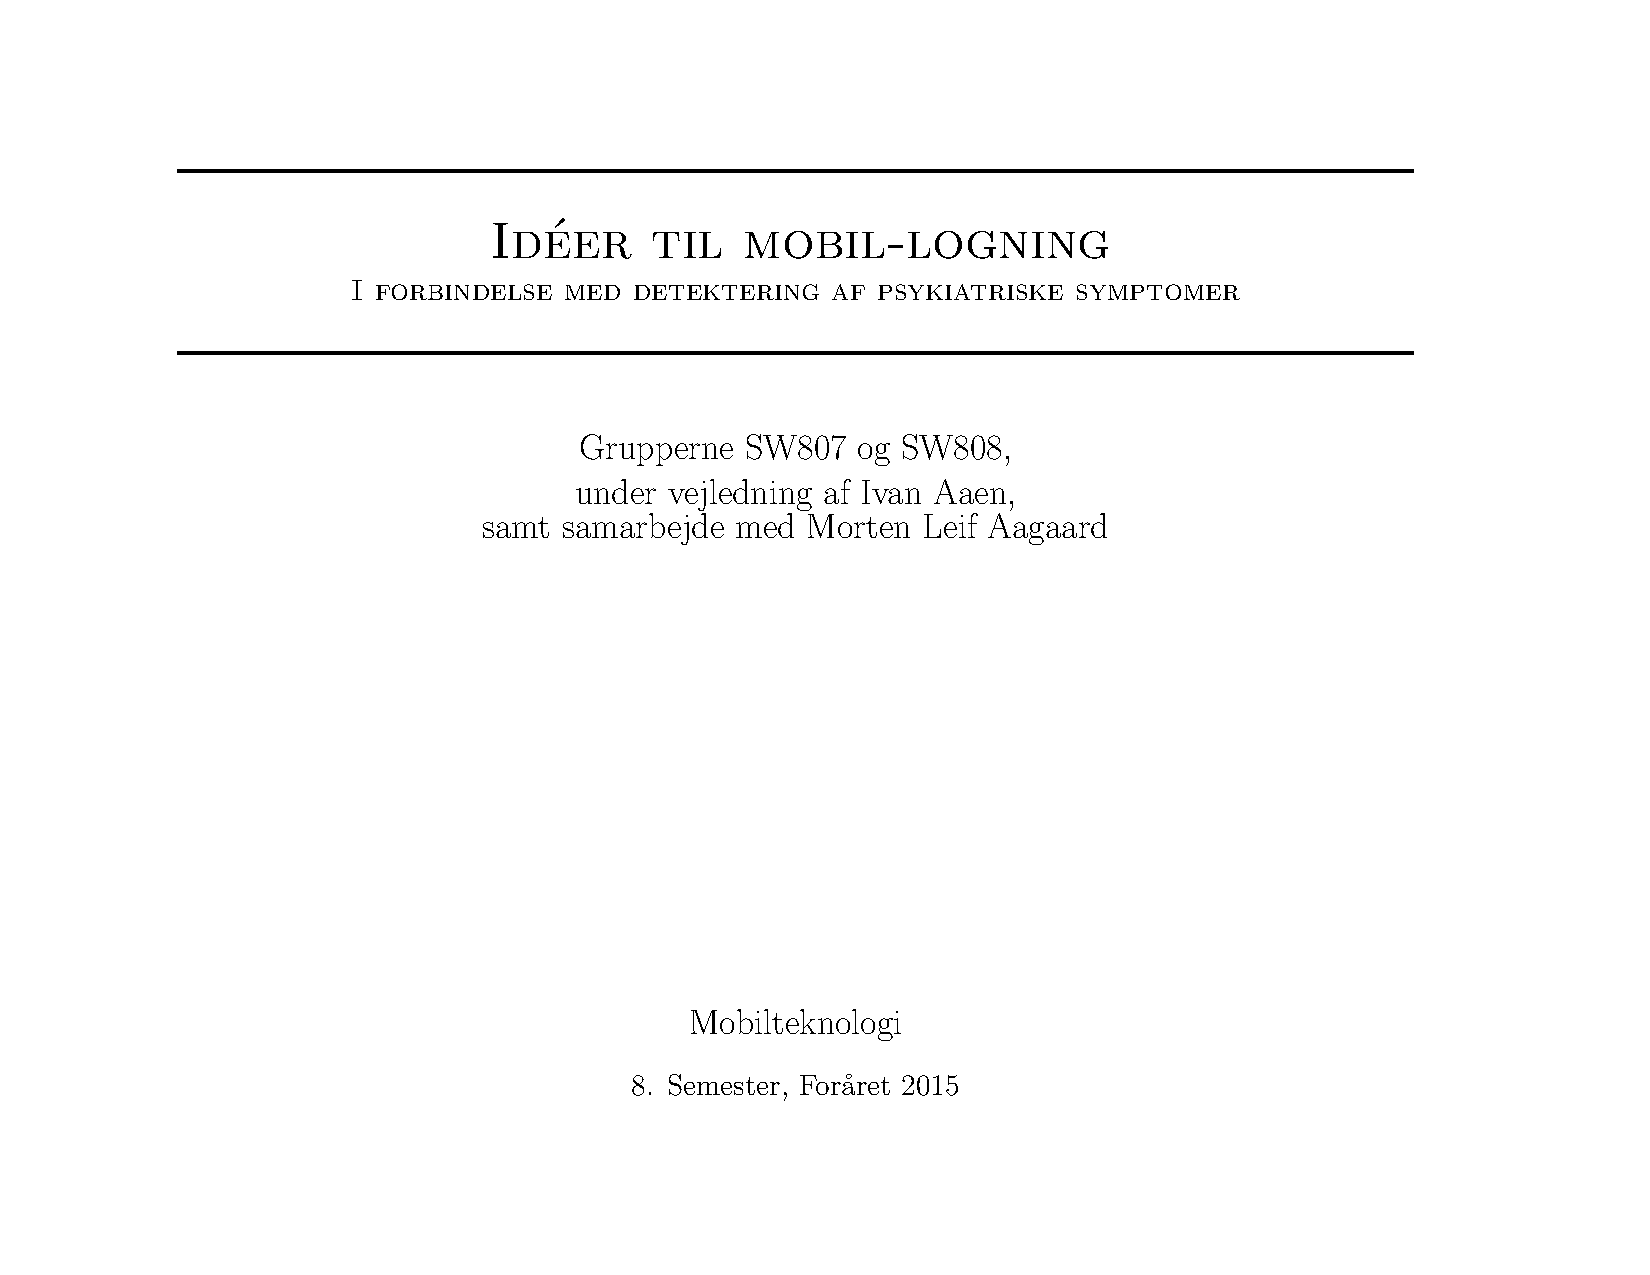
\includepdf[pages=-, nup=1x2]{appendix/brochurefil.pdf} 

\chapter{Stemningsregistrering}\label{app:stemningsregistrering}
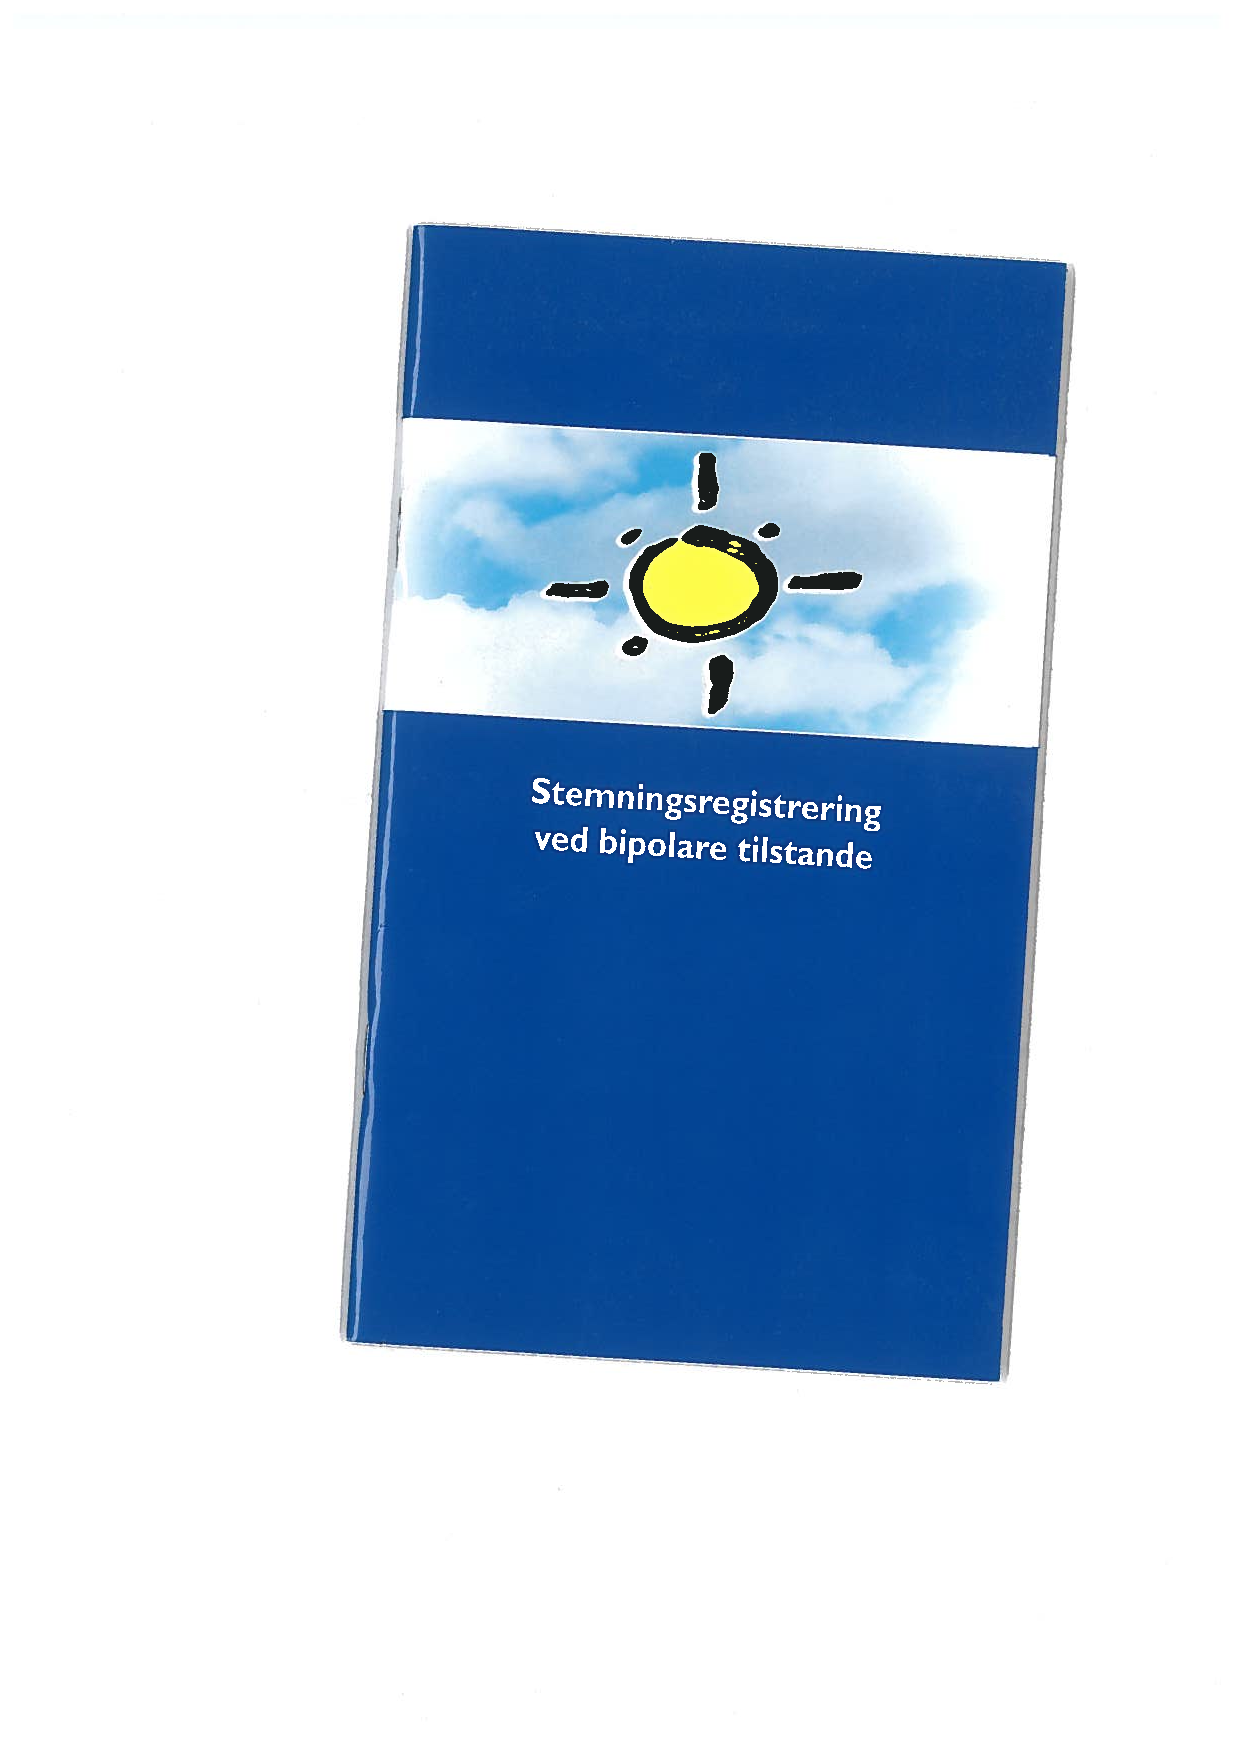
\includepdf[pages=-]{appendix/stemningsregistrering.pdf}
\end{document}
